%%%%%%%%%%%%%%%%%%%%%%%%%%%%%%%%%%%%%%%%%%%%%%%%%%%%%%%%%%%%%%%%%%%%%%%%%%%%%%
\documentclass[aspectratio=169]{beamer}            % Generate slides
%\documentclass[handout]{beamer}   % Generate handouts (6 slides to 1 page)
%\documentclass[aspectratio=169]{beamer}  % Use widescreen 16:9 aspect ratio
    % Possible aspect ratios are 16:9, 16:10, 14:9, 5:4, 4:3 (default) and 3:2
    % (Remember to remove the colon)

\usetheme{UoB}
%\usetheme[compress]{UoB}     % Compress the margins
%\usetheme[nourl]{UoB}        % Remove the footer with the URL
%\usetheme[nowatermark]{UoB}  % Remove the watermark from the title page

% Generate handouts with notes (3 slides + 3 notes to 1 page)
%\mode<handout>{
%  \pgfpagesuselayout{3 on 1 with notes}[a4paper,border shrink=10mm]
%}

\usepackage{nomencl} % nomenclature generation via makeindex
	\makenomenclature
\usepackage{tikz}
\usetikzlibrary{matrix,chains,scopes,arrows,positioning,fit,
	decorations.pathmorphing,decorations.markings,shapes,calc,
	positioning,patterns}
\usepackage[binary-units = true]{siunitx}
\usepackage{subfig}

\usepackage{pgfplots}
\pgfplotsset{compat=1.15}

\usepackage{pgfpages}
\usepackage{multimedia}

\mode<handout>{%
  \pgfpagesuselayout{4 on 1}[a4paper,landscape,border shrink=5mm] 
	\setbeamercolor{background canvas}{bg=black!5}
  %\setbeameroption{show notes}
}

\mode<second>{%
  \setbeameroption{show notes on second screen}
}

\everymath{\displaystyle}

\graphicspath{{./Figures/}}

%%%%%%%%%%%%%%%%%%%%%%%%%%%%%%%%%%%%%%%%%%%%%%%%%%%%%%%%%%%%%%%%%%%%%%%%%%%%%%
\title[Bio-Inspired Distributed Sensing]{Bio-Inspired Distributed Sensing for
	Improved Flight Control}
%\subtitle{Subtitle}
\author{Sergio A. Araujo-Estrada}
\institute{Research Associate \\
	Aerospace Engineering Department \\
	\href{mailto:s.araujoestrada@bristol.ac.uk}{s.araujoestrada@bristol.ac.uk}}
\date{Thursday, May 3}

%%%%%%%%%%%%%%%%%%%%%%%%%%%%%%%%%%%%%%%%%%%%%%%%%%%%%%%%%%%%%%%%%%%%%%%%%%%%%%
\begin{document}

\setbeamercovered{transparent}

\titlepage

%%%%%%%%%%%%%%%%%%%%%%%%%%%%%%%%%%%%%%%%%%%%%%%%%%%%%%%%%%%%%%%%%%%%%%%%%%%%%%
\begin{frame}{Overview}
	\tableofcontents
\end{frame}

%%%%%%%%%%%%%%%%%%%%%%%%%%%%%%%%%%%%%%%%%%%%%%%%%%%%%%%%%%%%
\section{Introduction}
\subsection{Motivation}
\begin{frame}{Motivation: Why Bio-Inspired Distributed Sensing?}

  \centering
  \movie[externalviewer]{%
	  {\centering\color{blue}Amazing Kestrel!!!}}
    {./Videos/KestrelHovering&Hunting_Cornwall.mp4}
	\\[1em]
	Kestrel Hovering and Hunting in Cornwall\\
	Paul Dinning, 2015\\
	\url{https://www.youtube.com/watch?v=7j6OsP7zL6w}

  \note[item]{Head is stationary}
  \note[item]{Wing morphing}
	\note[item]{Tail morphing}
	\note[item]{Compare \& contrast with UAVs}
	\note[item]{Control strategies:\\
	  a) Inertial \& visual control\\
		b) What other senses is the kestrel using?
	}

\end{frame}

%%%%%%%%%%%%%%%%%%%%%%%%%%%%%%%%%%%%%%%%%%%%%%%%%%%%%%%%%%%%
\begin{frame}[plain]{Motivation: Why Bio-Inspired Distributed Sensing?}

  \begin{figure}[!htb]
    \centering
		% BioSystemsSensing.tex

\tikzstyle{LabelObject}=[fill=white,rectangle,align=center]
\tikzstyle{Block}=[rectangle,draw=blue,rounded corners,line width=0.5mm,
  align=center,minimum height=12em,minimum width=32em]

\resizebox{!}{0.4\textwidth}{
	\begin{tikzpicture}[x=1.25cm, y=1.25cm, >=stealth]
		%\draw[help lines,xstep=.5,ystep=.5] (-9,-10) grid (15,3);
		%\foreach \x in {-9,-8,...,15} { \node [anchor=north] at (\x/1,0) {0.\x}; }
		%\foreach \y in {-10,-9,...,3} { \node [anchor=east] at (0,\y/1) {0.\y}; }
	  %
		\begin{scope}
			\node[anchor=center,inner sep=0] (image11) at (0,0)%
				{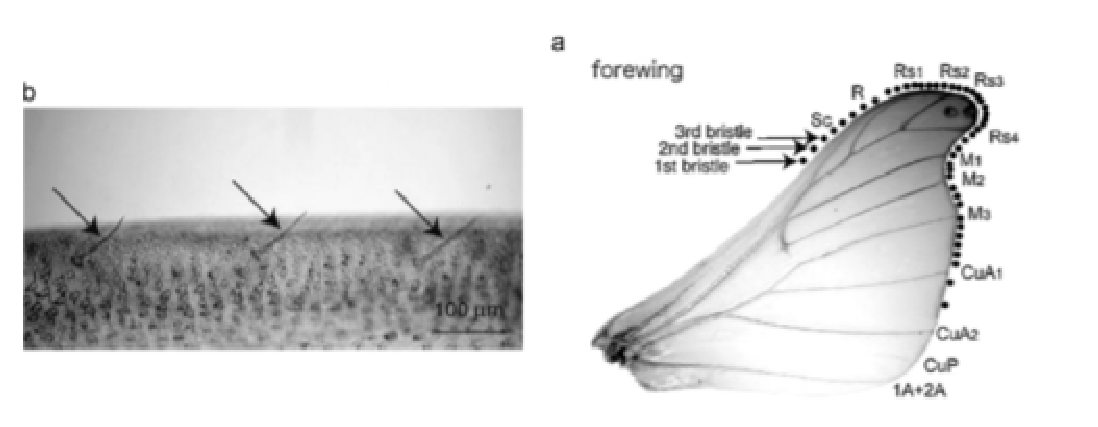
\includegraphics[height=0.25\textwidth]{Yoshida_InsectHairs.eps}};
		\end{scope}
		\begin{scope}
			\node[anchor=center,inner sep=0] (image21) at (0,-4)%
				{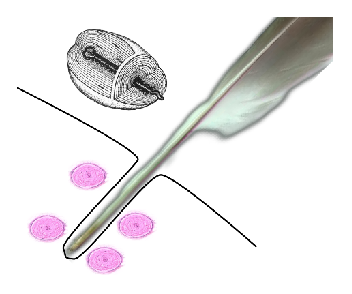
\includegraphics[height=0.25\textwidth]{HerbstCorpuscles.eps}};
		\end{scope}
		\begin{scope}
			\node[anchor=center,inner sep=0] (image31) at (0,-8)%
				{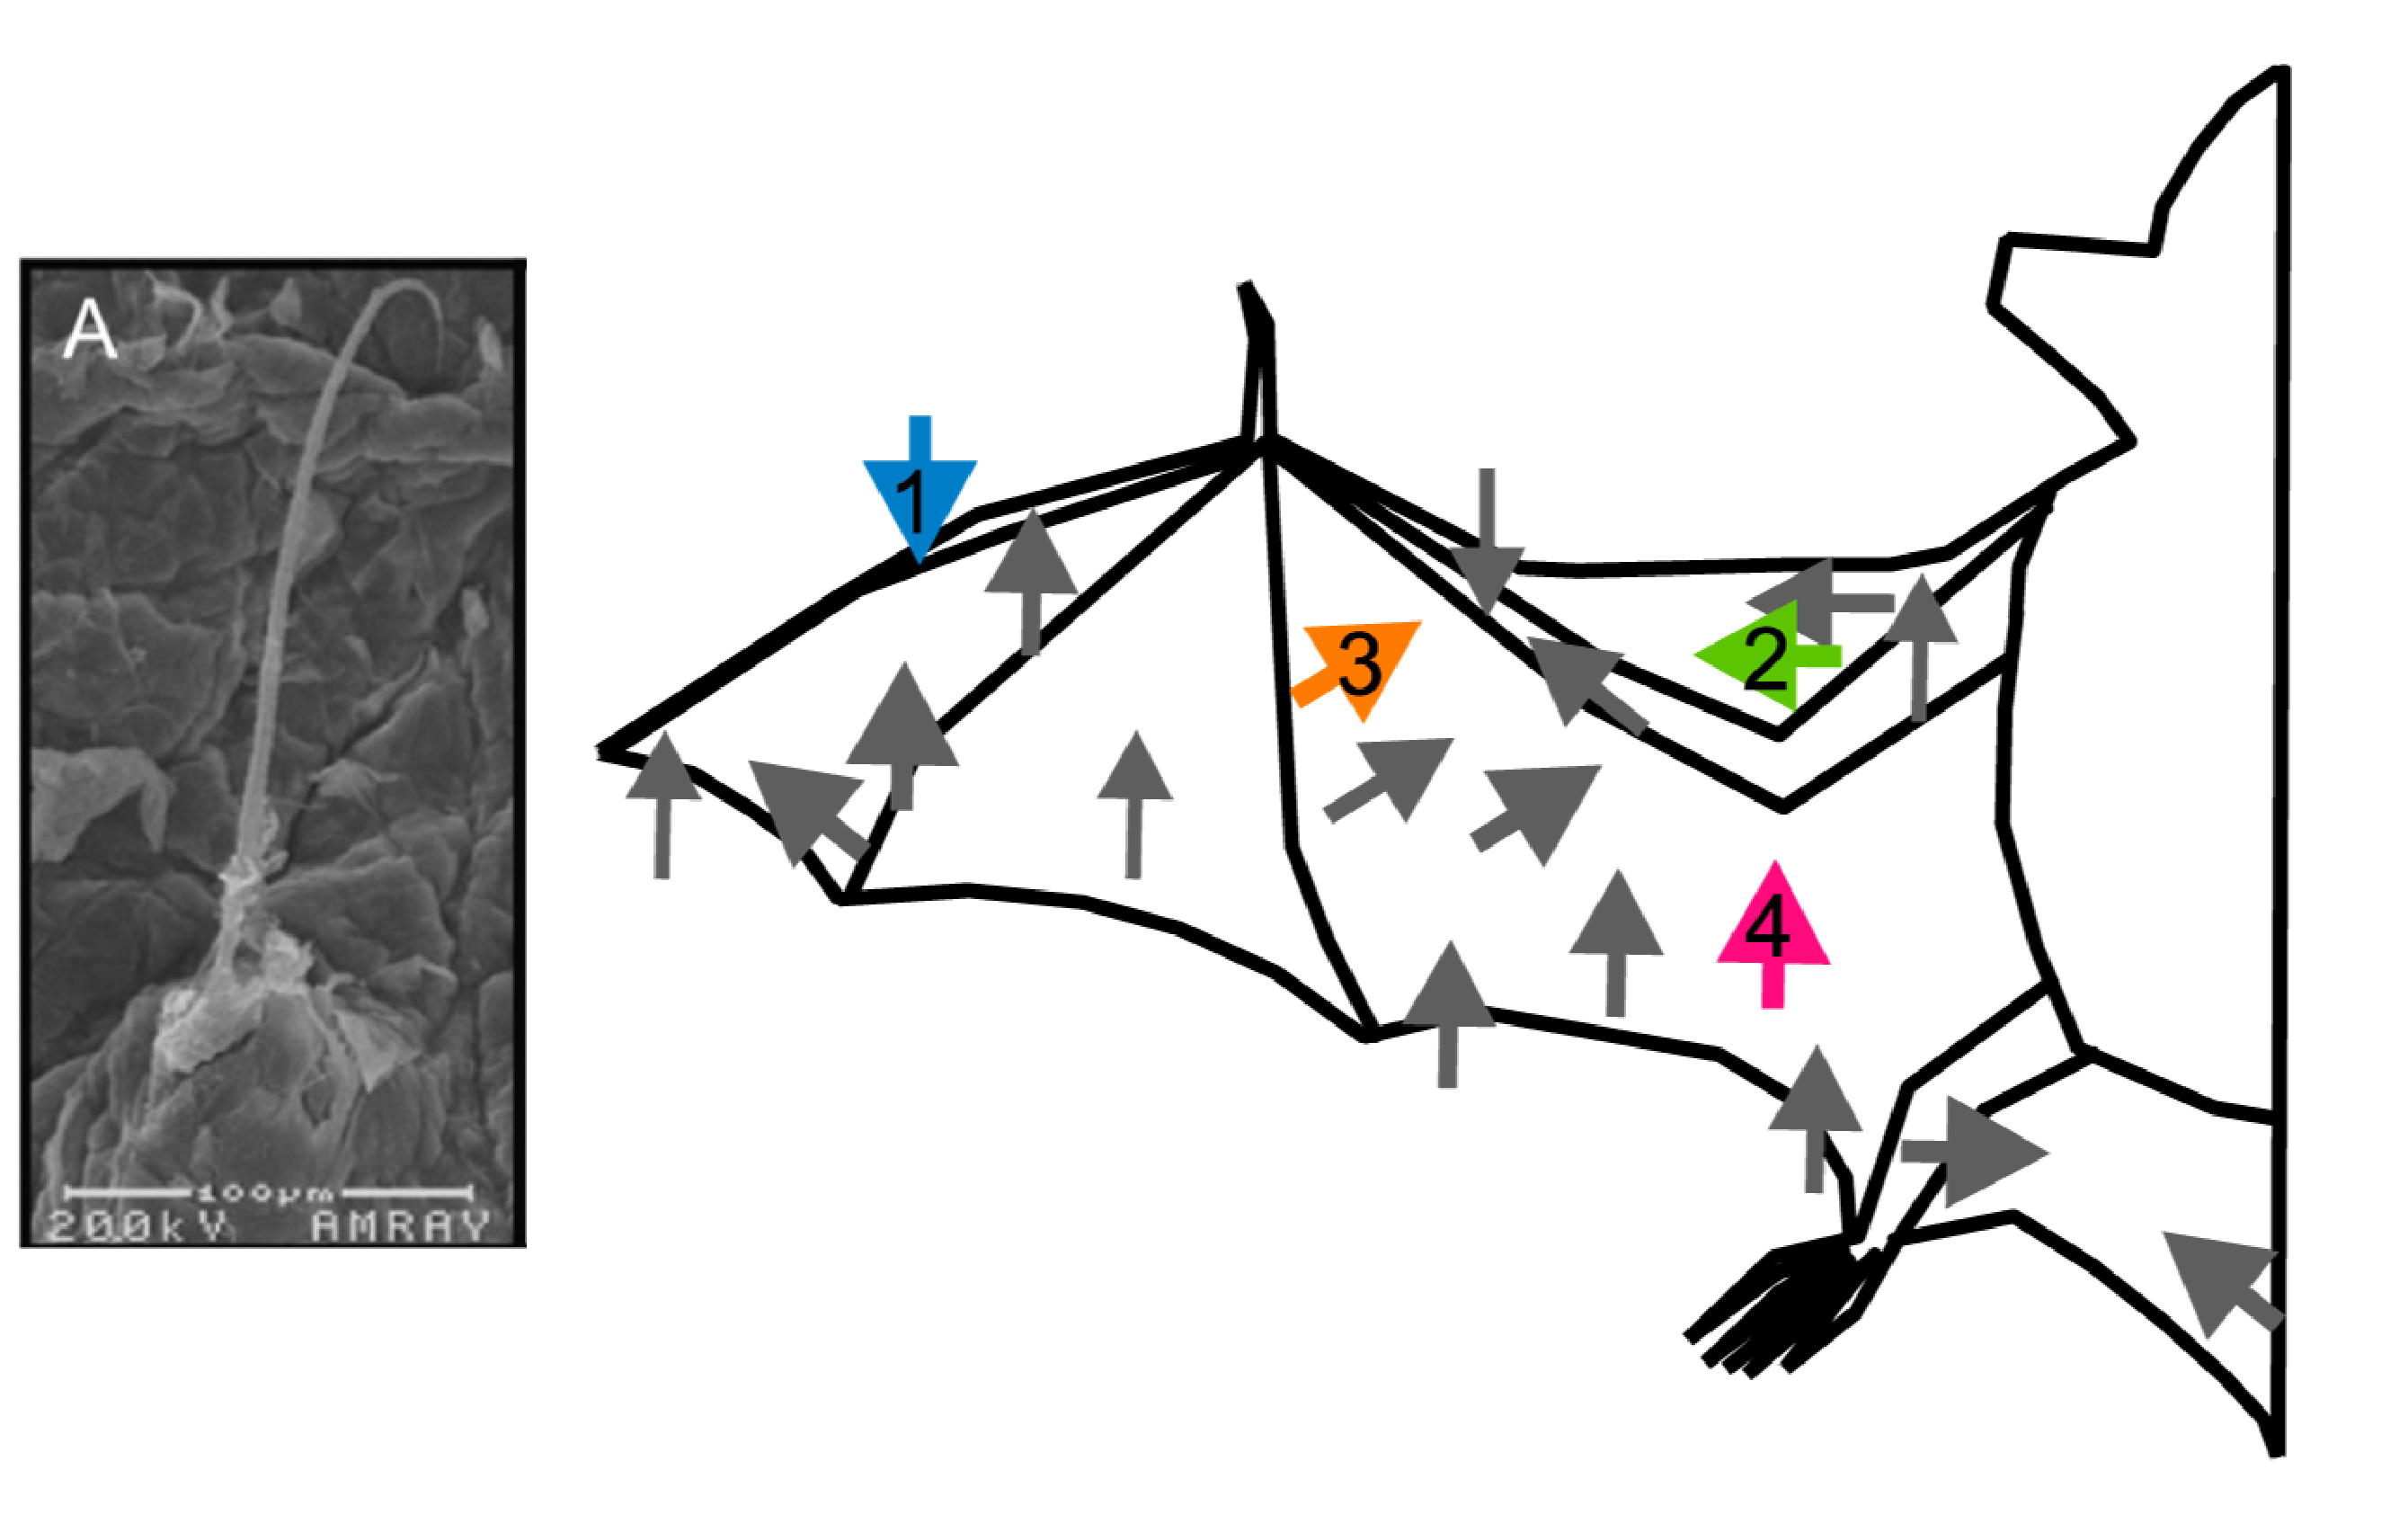
\includegraphics[height=0.25\textwidth]{SterbingDAngelo_BatHairs.eps}};
		\end{scope}
		%
		\begin{scope}
		  \node[anchor=center,inner sep=0] (image12) at (10,0)%
				{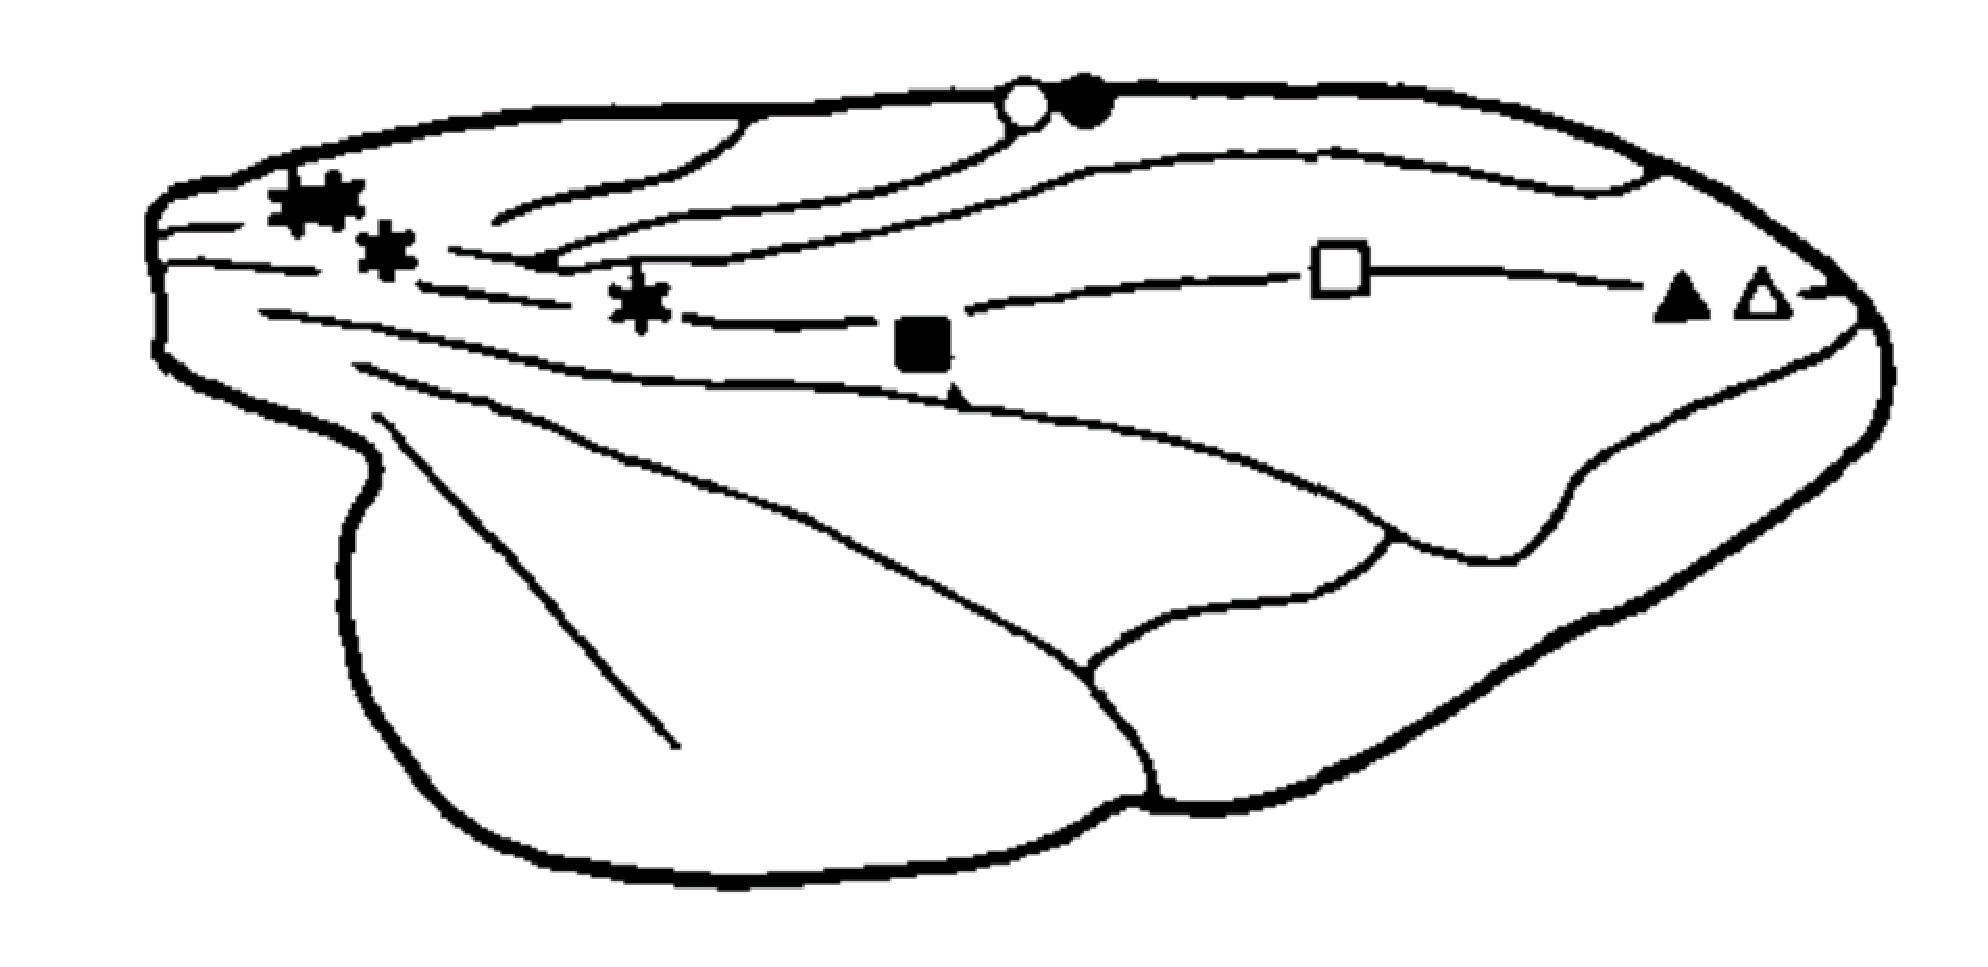
\includegraphics[height=0.25\textwidth]{Dickinson_Fly_CampaniformSensilla.eps}};
		\end{scope}
		\begin{scope}
		  \node[anchor=center,inner sep=0] (image22) at (10,-4)%
				{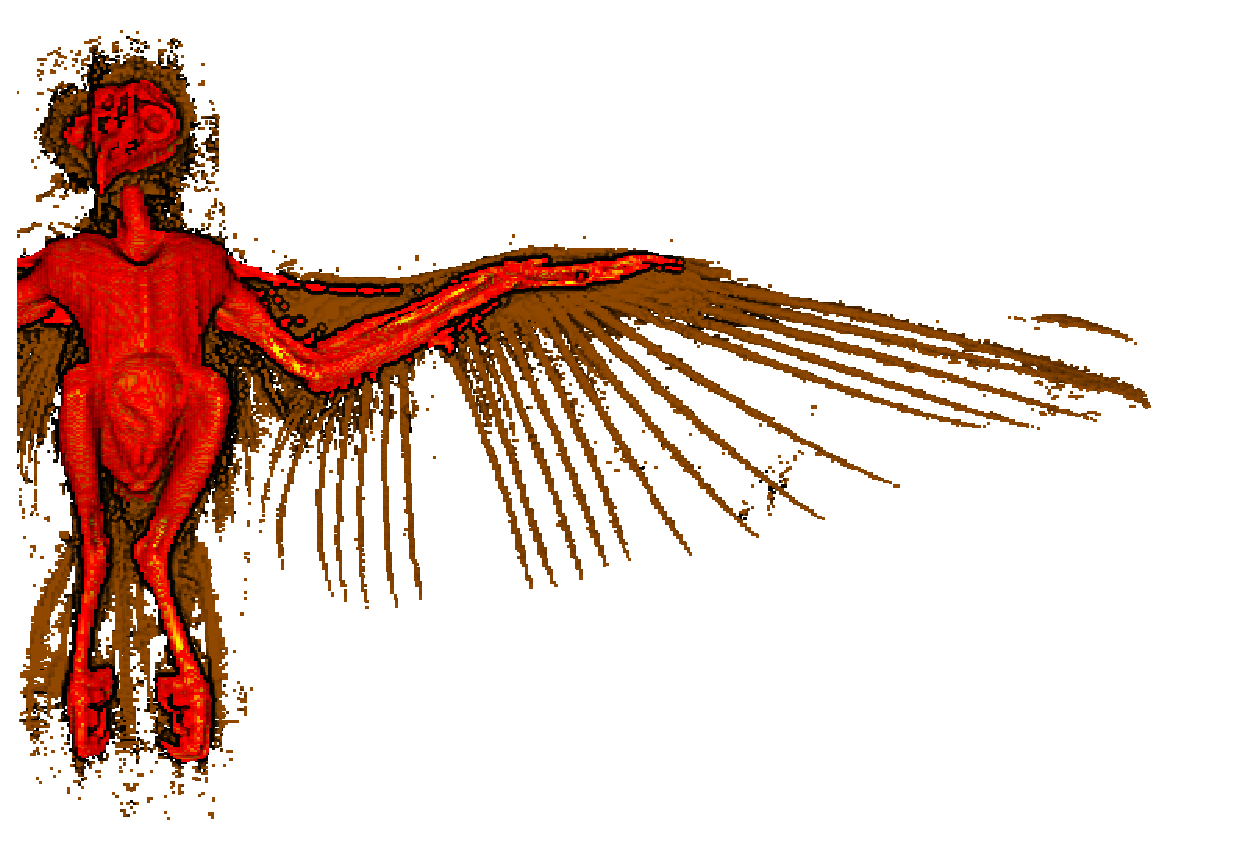
\includegraphics[height=0.25\textwidth]{BarnOwlCT_MuscleFeatherOffset.eps}};
		\end{scope}
		\begin{scope}
		  \node[anchor=center,inner sep=0] (image32) at (10,-8)%
				{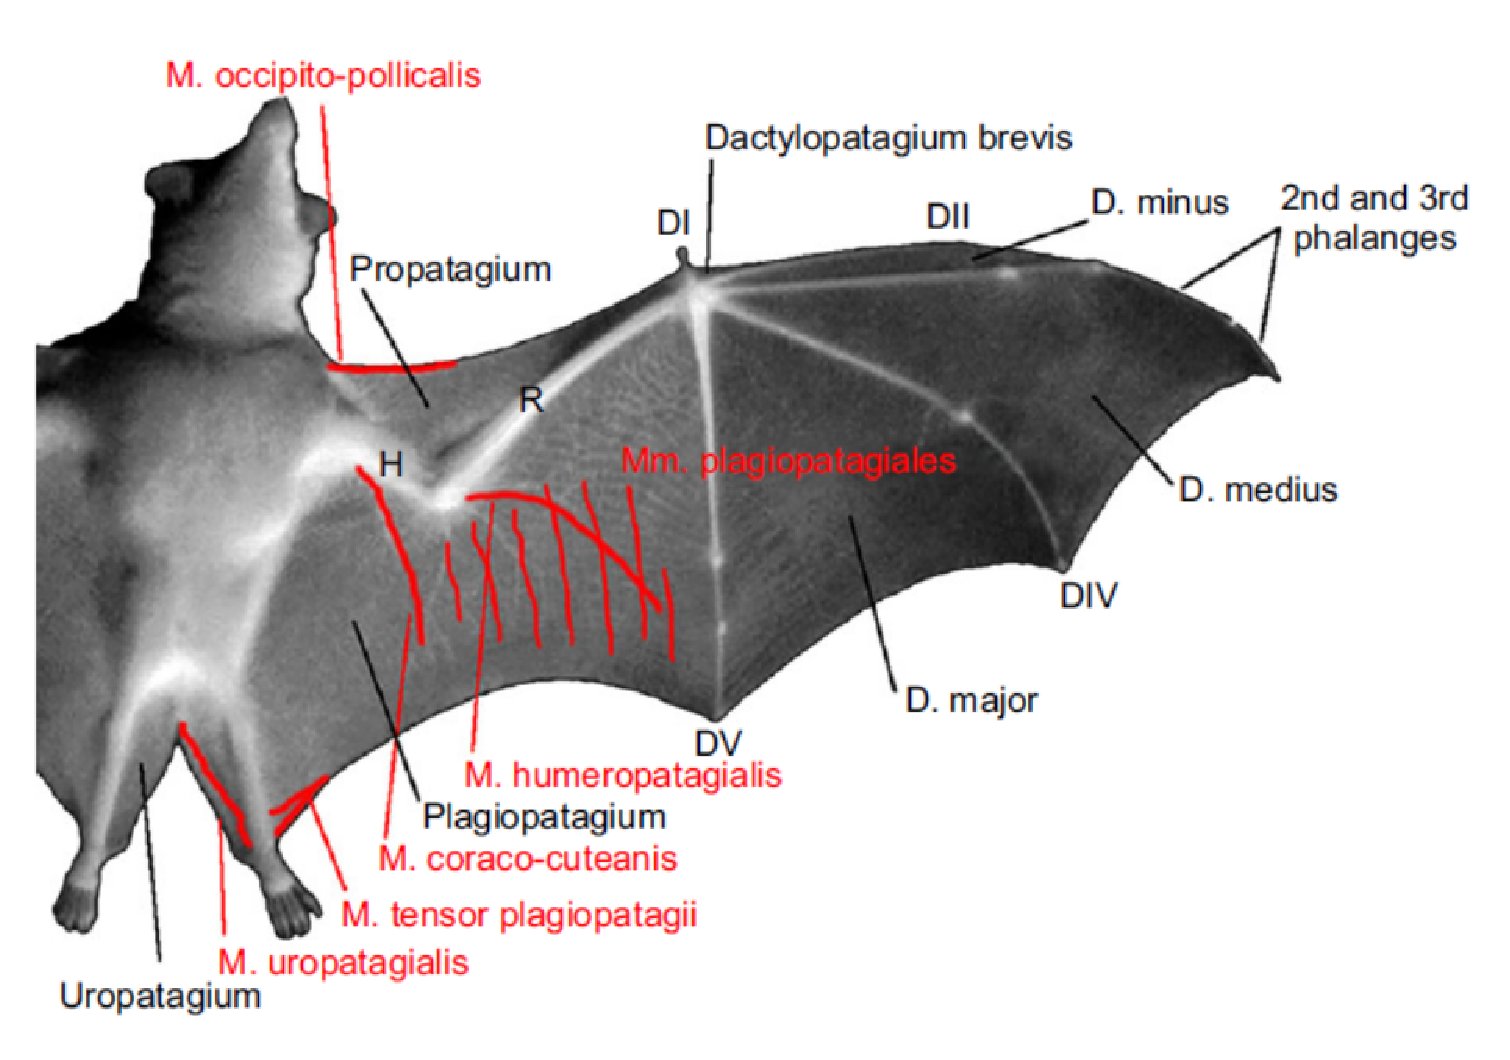
\includegraphics[height=0.25\textwidth]{Bat_MuscleSpindles.eps}};
		\end{scope}
		%
		\draw(image11.north) ++(0,1) node (FlowSens_Label) {\Huge{\bf Flow Sensors}};
		\draw(image12.north) ++(0,1) node (ForceSens_Label) {\Huge{\bf Force Sensors}};
		\draw(image11.west) ++(-6, 0) node (Insects_Label) {\Huge{\bf Insects}};
		\draw(image11.west) ++(-6,-4) node (Birds_Label) {\Huge{\bf Birds}};
		\draw(image11.west) ++(-6,-8) node (Bats_Label) {\Huge{\bf Bats}};
		%
		\draw(image11.north west) ++(2.5,-0.5) node[LabelObject] (InsectHairs_Label) {Silkworm moth: Bristles/Hairs};
		\draw(image11.south west) ++(2.5,0.0) node[gray,LabelObject] (InsectHairsAuthor_Label) {Ai et al. (2010)};
		\draw(image12.east) ++(1,  0) node[LabelObject] (InsectCampSens_Label) {Blowfly:\\Campaniform\\sensilla};
		\draw(image12.east) ++(1, -1) node[gray,LabelObject] (InsectCampSensAuthor_Label) {Dickinson (1990)};
		
		\draw(image21.west) ++(-1,  0) node[LabelObject] (HerbstCorpuscles_Label) {Herbst\\corpuscles};
		\draw(image22.east) ++(1,  0) node[LabelObject] (BirdSpindles_Label) {Muscle\\spindles};
		
		\draw(image31.west) ++(-1,  0) node[LabelObject] (BatHairs_Label) {Hairs};
		\draw(image31.west) ++( 1, -1.5) node[gray,LabelObject] (BatHairsAuthor_Label) {Sterbing-D'Angeloa et al. (2011)};
		\draw(image32.east) ++(1,  0) node[LabelObject] (BatSpindles_Label) {Muscle\\spindles};
		\draw(image32.east) ++(1, -1) node[gray,LabelObject] (BatSpindlesAuthor_Label) {Hedenstrom et al. (2015)};
		
		
		\only<2>{
		  % Sensing system 11
		  \draw(image11) node[Block] (SensSystem11) {};
		}
		\only<3>{
		  % Sensing system 12
		  \draw(image12) +(0.9,0) node[Block] (SensSystem12) {};
		}
		\only<4>{
		  % Sensing system 21
		  \draw(image21) node[Block] (SensSystem21) {};
		}
		\only<5>{
		  % Sensing system 22
		  \draw(image22) +(0.9,0) node[Block] (SensSystem22) {};
		}
		\only<6>{
		  % Sensing system 31
		  \draw(image31) node[Block] (SensSystem31) {};
		}
		\only<7>{
		  % Sensing system 32
		  \draw(image32) +(0.9,0) node[Block] (SensSystem32) {};
		}
		
	\end{tikzpicture}
}
		\caption{Biological systems sensing}
		\label{fig:BioSystemsSensing}
  \end{figure}
	
	\note{... Herbst corpuscles are vibration-sensitive mechano-receptors with broad bandpass tuning curves.}

\end{frame}

%%%%%%%%%%%%%%%%%%%%%%%%%%%%%%%%%%%%%%%%%%%%%%%%%%%%%%%%%%%%
\begin{frame}{Motivation: Why Bio-Inspired Distributed Sensing?}
  
  \pause
  \begin{columns}
    \begin{column}{0.5\textwidth}
      \begin{itemize}
	      \item<1->{Current UAV autopilot technologies}\\[4em]
	      \item<3->{Challenges}\\[4em]
	      \item<5->{Potential use of force and flow information}\\[4em]
      \end{itemize}
    \end{column}
    \begin{column}{0.5\textwidth}  %%<--- here
      \only<2>{
	\begin{itemize}
	  \item[-]{Inertial}
	  \item[-]{Single point air speed}
	  \item[-]{GPS}
	  \item[-]{Vision}
	\end{itemize}
      }
      \only<4>{
	\begin{itemize}
	  \item[-]Intrinsic nonlinear dynamics
	  \item[-]Classic control strategies limitations
	  \item[-]Limitations of inertial controls
	\end{itemize}	  
      }
      \only<6>{

	\begin{itemize}
	  \item[-]Availability of aerodynamic variables
	  \begin{itemize}
      \item[${\rightarrow}$]Improved flight dynamics model
      \item[${\rightarrow}$]Stall detection
    \end{itemize}
	  \item[-]Earlier gust detection
		\begin{itemize}
		   \item[${\rightarrow}$]Gust rejection/alleviation
		\end{itemize}
		\item[-]Localised information
		\begin{itemize}
		   \item[${\rightarrow}$]Localised control
			\item[${\rightarrow}$]Load tailoring
    \end{itemize}
		
	  %\item[-]Aeroelastic effects
	  %\item[-]Additional 'hidden' information
	\end{itemize}
      }
    \end{column}
  \end{columns}
  
\end{frame}

%%%%%%%%%%%%%%%%%%%%%%%%%%%%%%%%%%%%%%%%%%%%%%%%%%%%%%%%%%%%
\subsection{Research Problem}
\begin{frame}{Research Problem}
  
	Use force and flow sensing to improve performance of UAVs flight control systems.\\
	\begin{columns}
    \begin{column}{0.35\textwidth}
      \pause
      To achieve this we aim to:
      \begin{itemize}
        \item<3-> Develop distributed sensing system for UAV
        \item<4-> Integrate with conventional flight control system
        \item<5-> Measure response to turbulence
        \item<6-> Develop flight control systems
      \end{itemize}
	  \end{column}
		\begin{column}{0.65\textwidth}
		  \only<3>{		
				\begin{figure}[!htb]
	  			\centering
	  			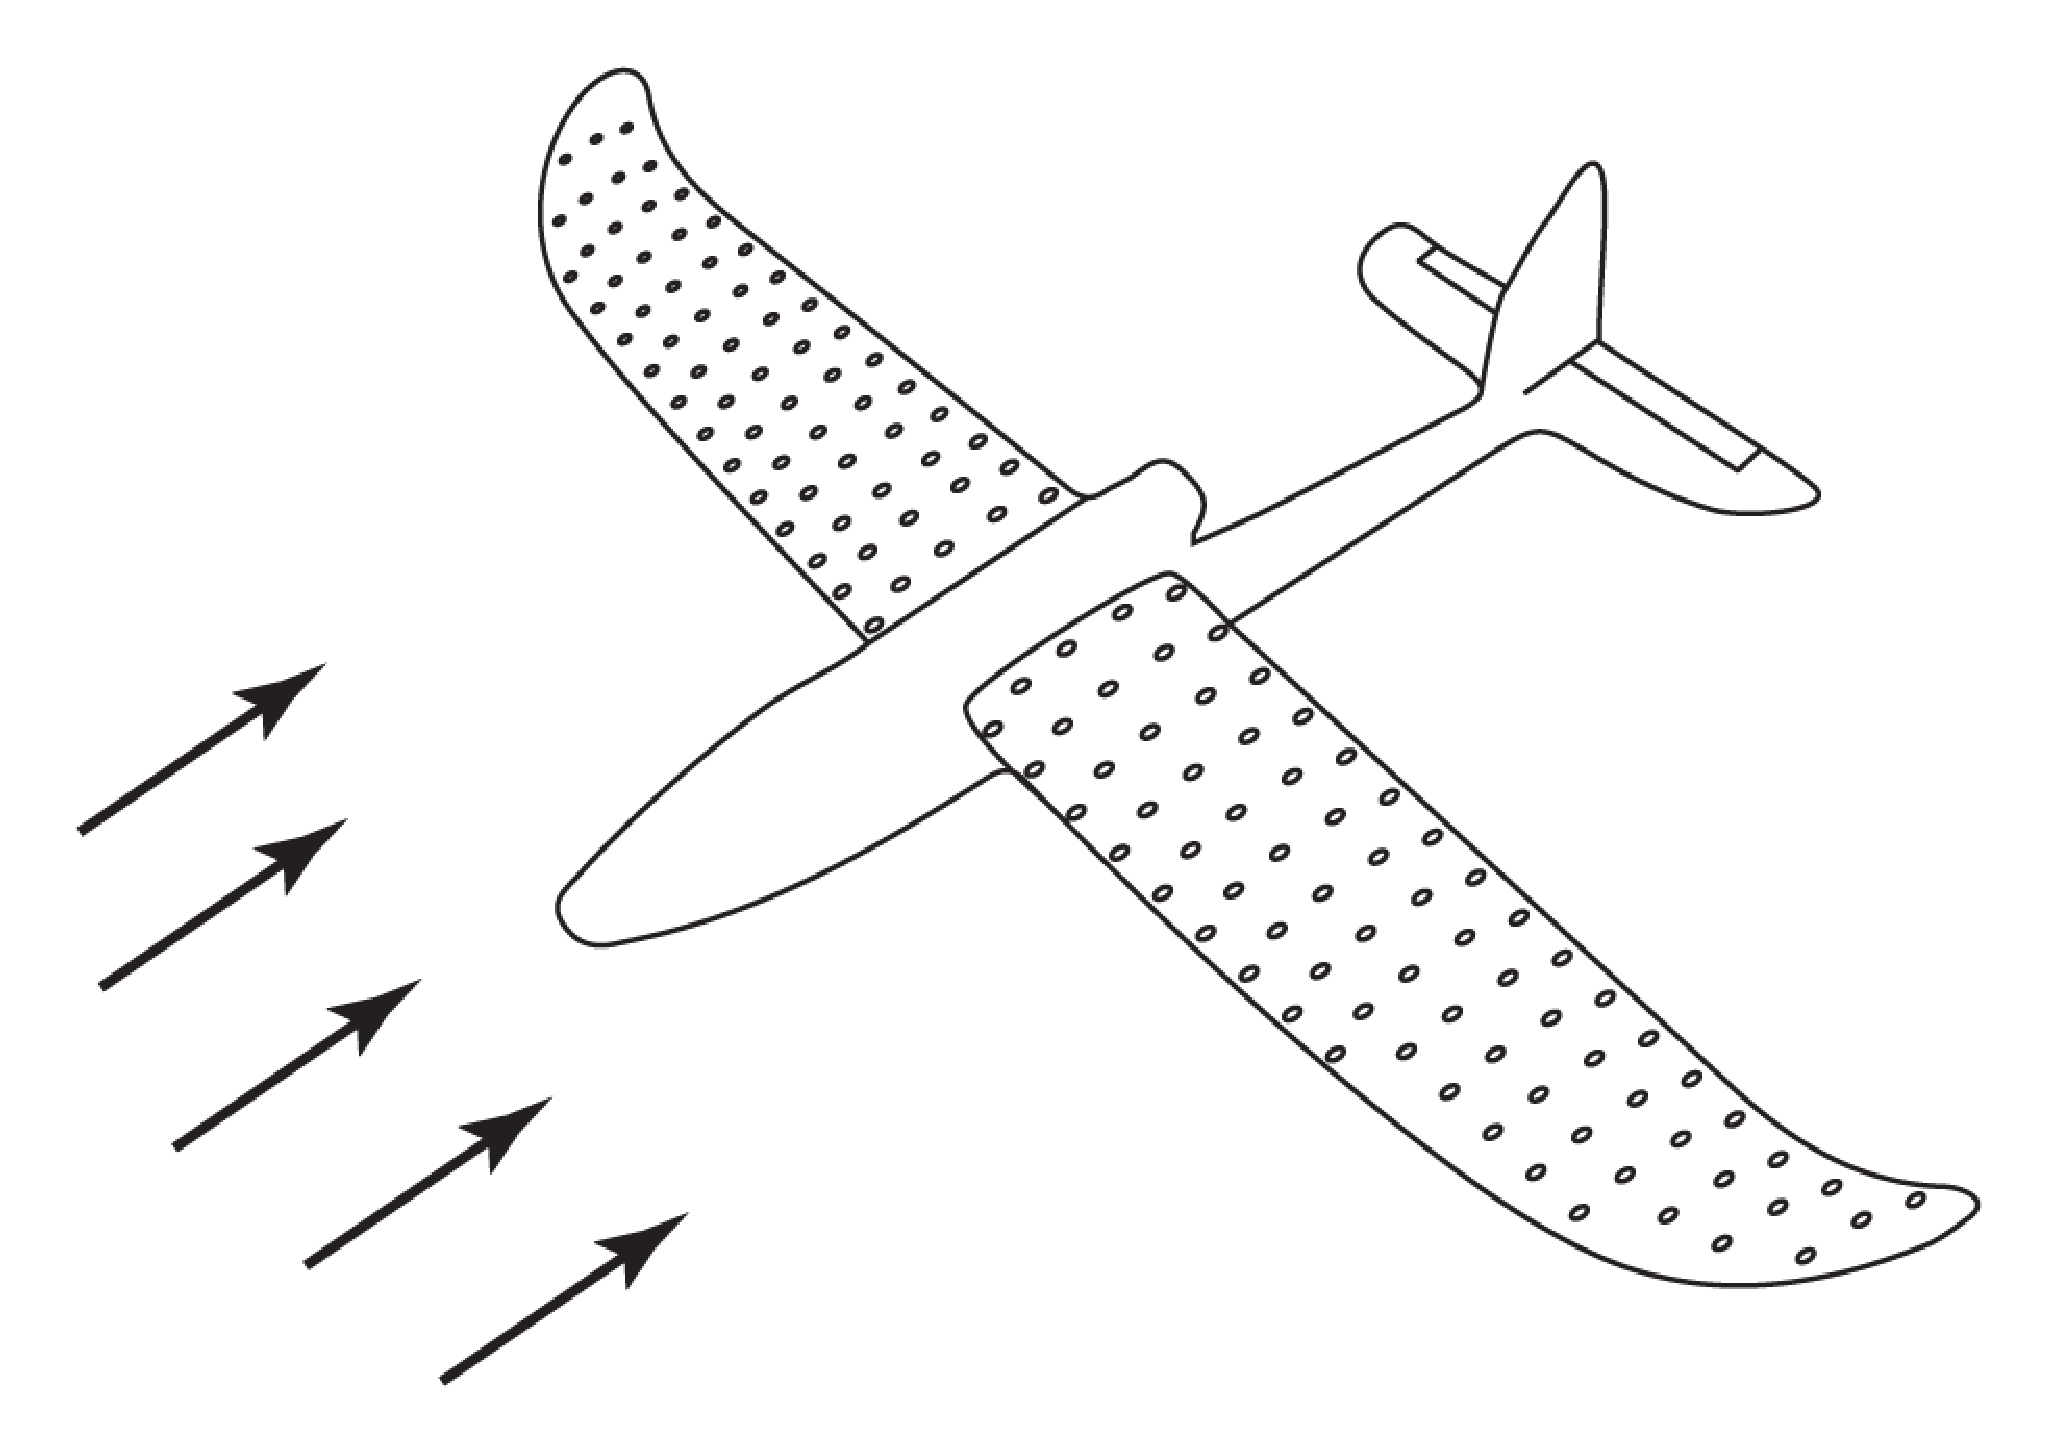
\includegraphics[height=0.45\textwidth]{DistSensingUAV.eps}
				\end{figure}
			}
			\only<4>{		
				\begin{figure}[!htb]
	  			\centering
	  			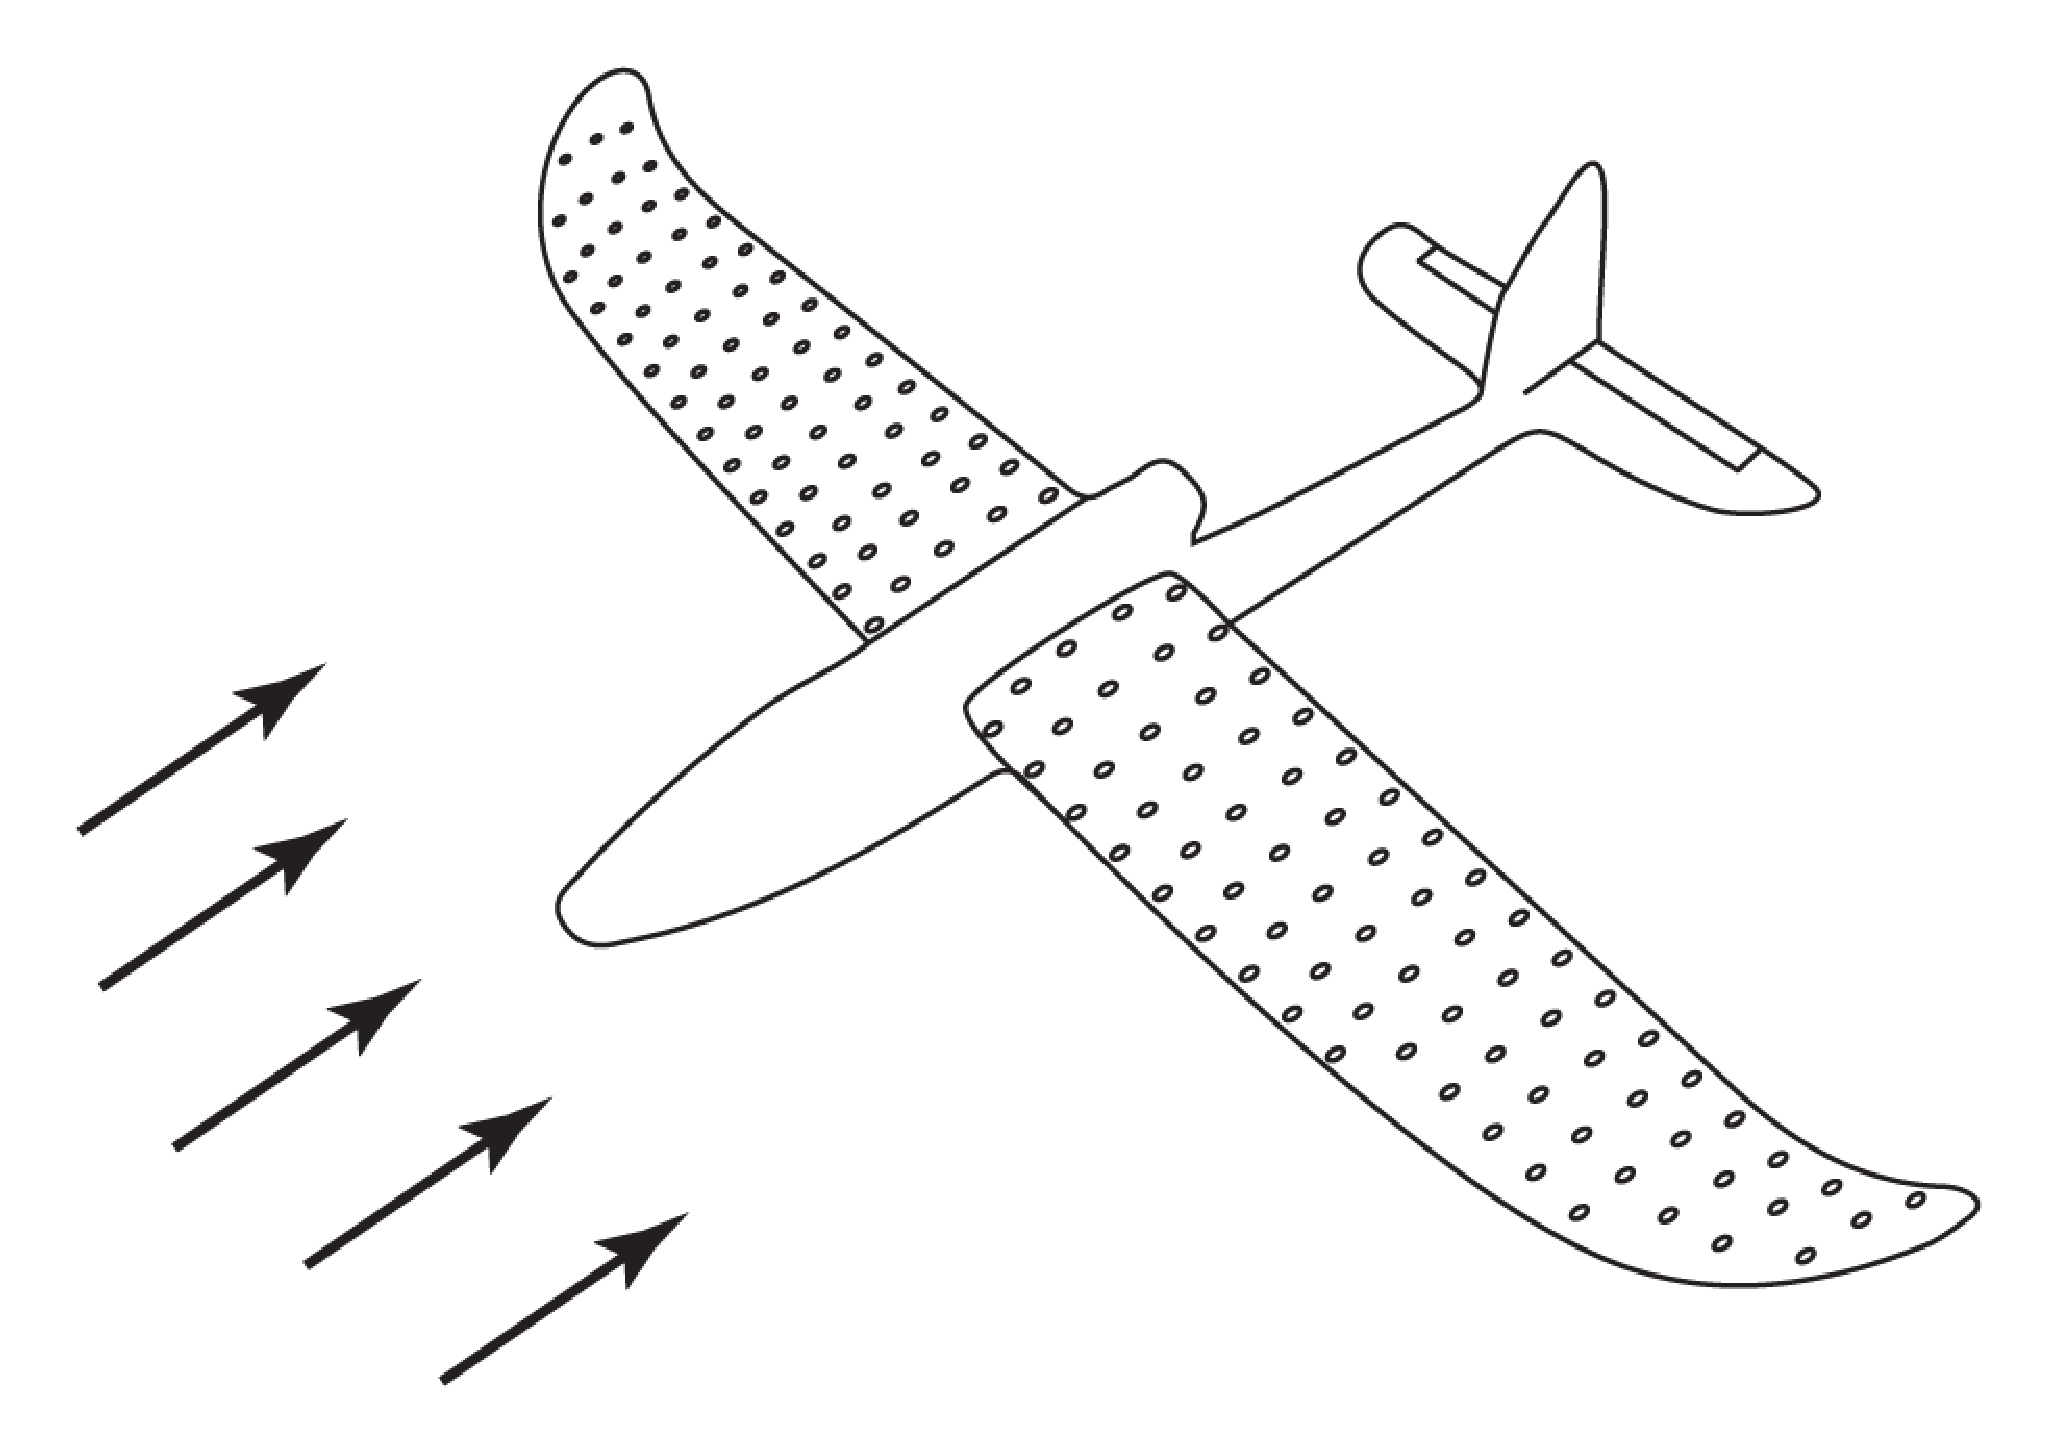
\includegraphics[height=0.45\textwidth]{DistSensingUAV.eps}
				\end{figure}
			}
			\only<5>{		
				\begin{figure}[!htb]
	  			\centering
	  			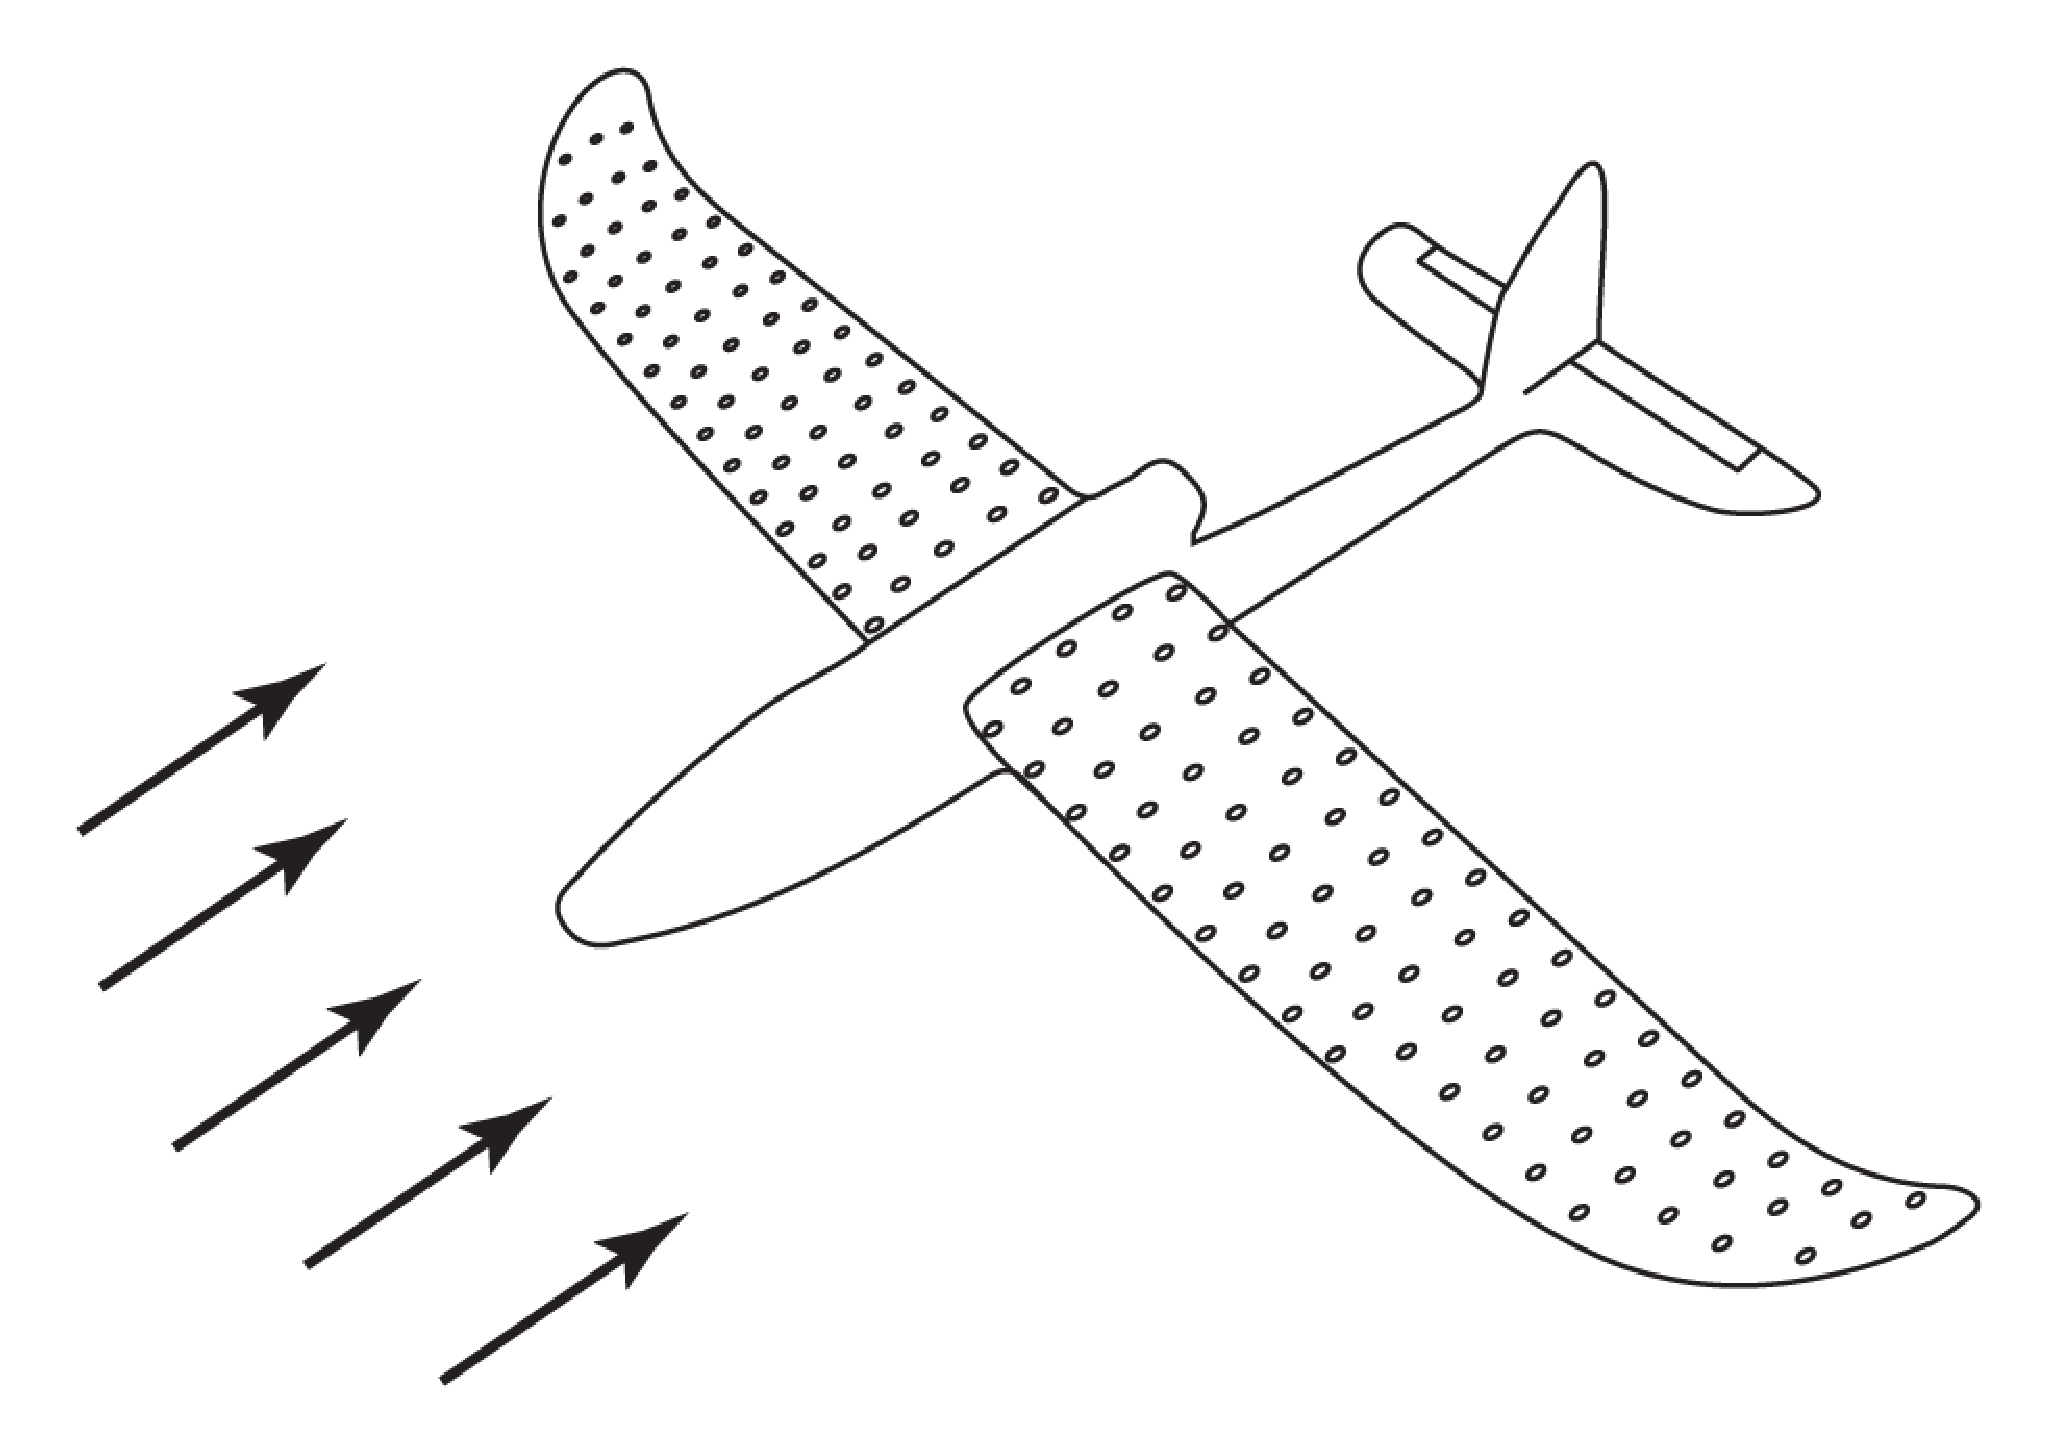
\includegraphics[height=0.45\textwidth]{DistSensingUAV.eps}
				\end{figure}
			}
			\only<6>{		
				\begin{figure}[!htb]
	  			\centering
	  			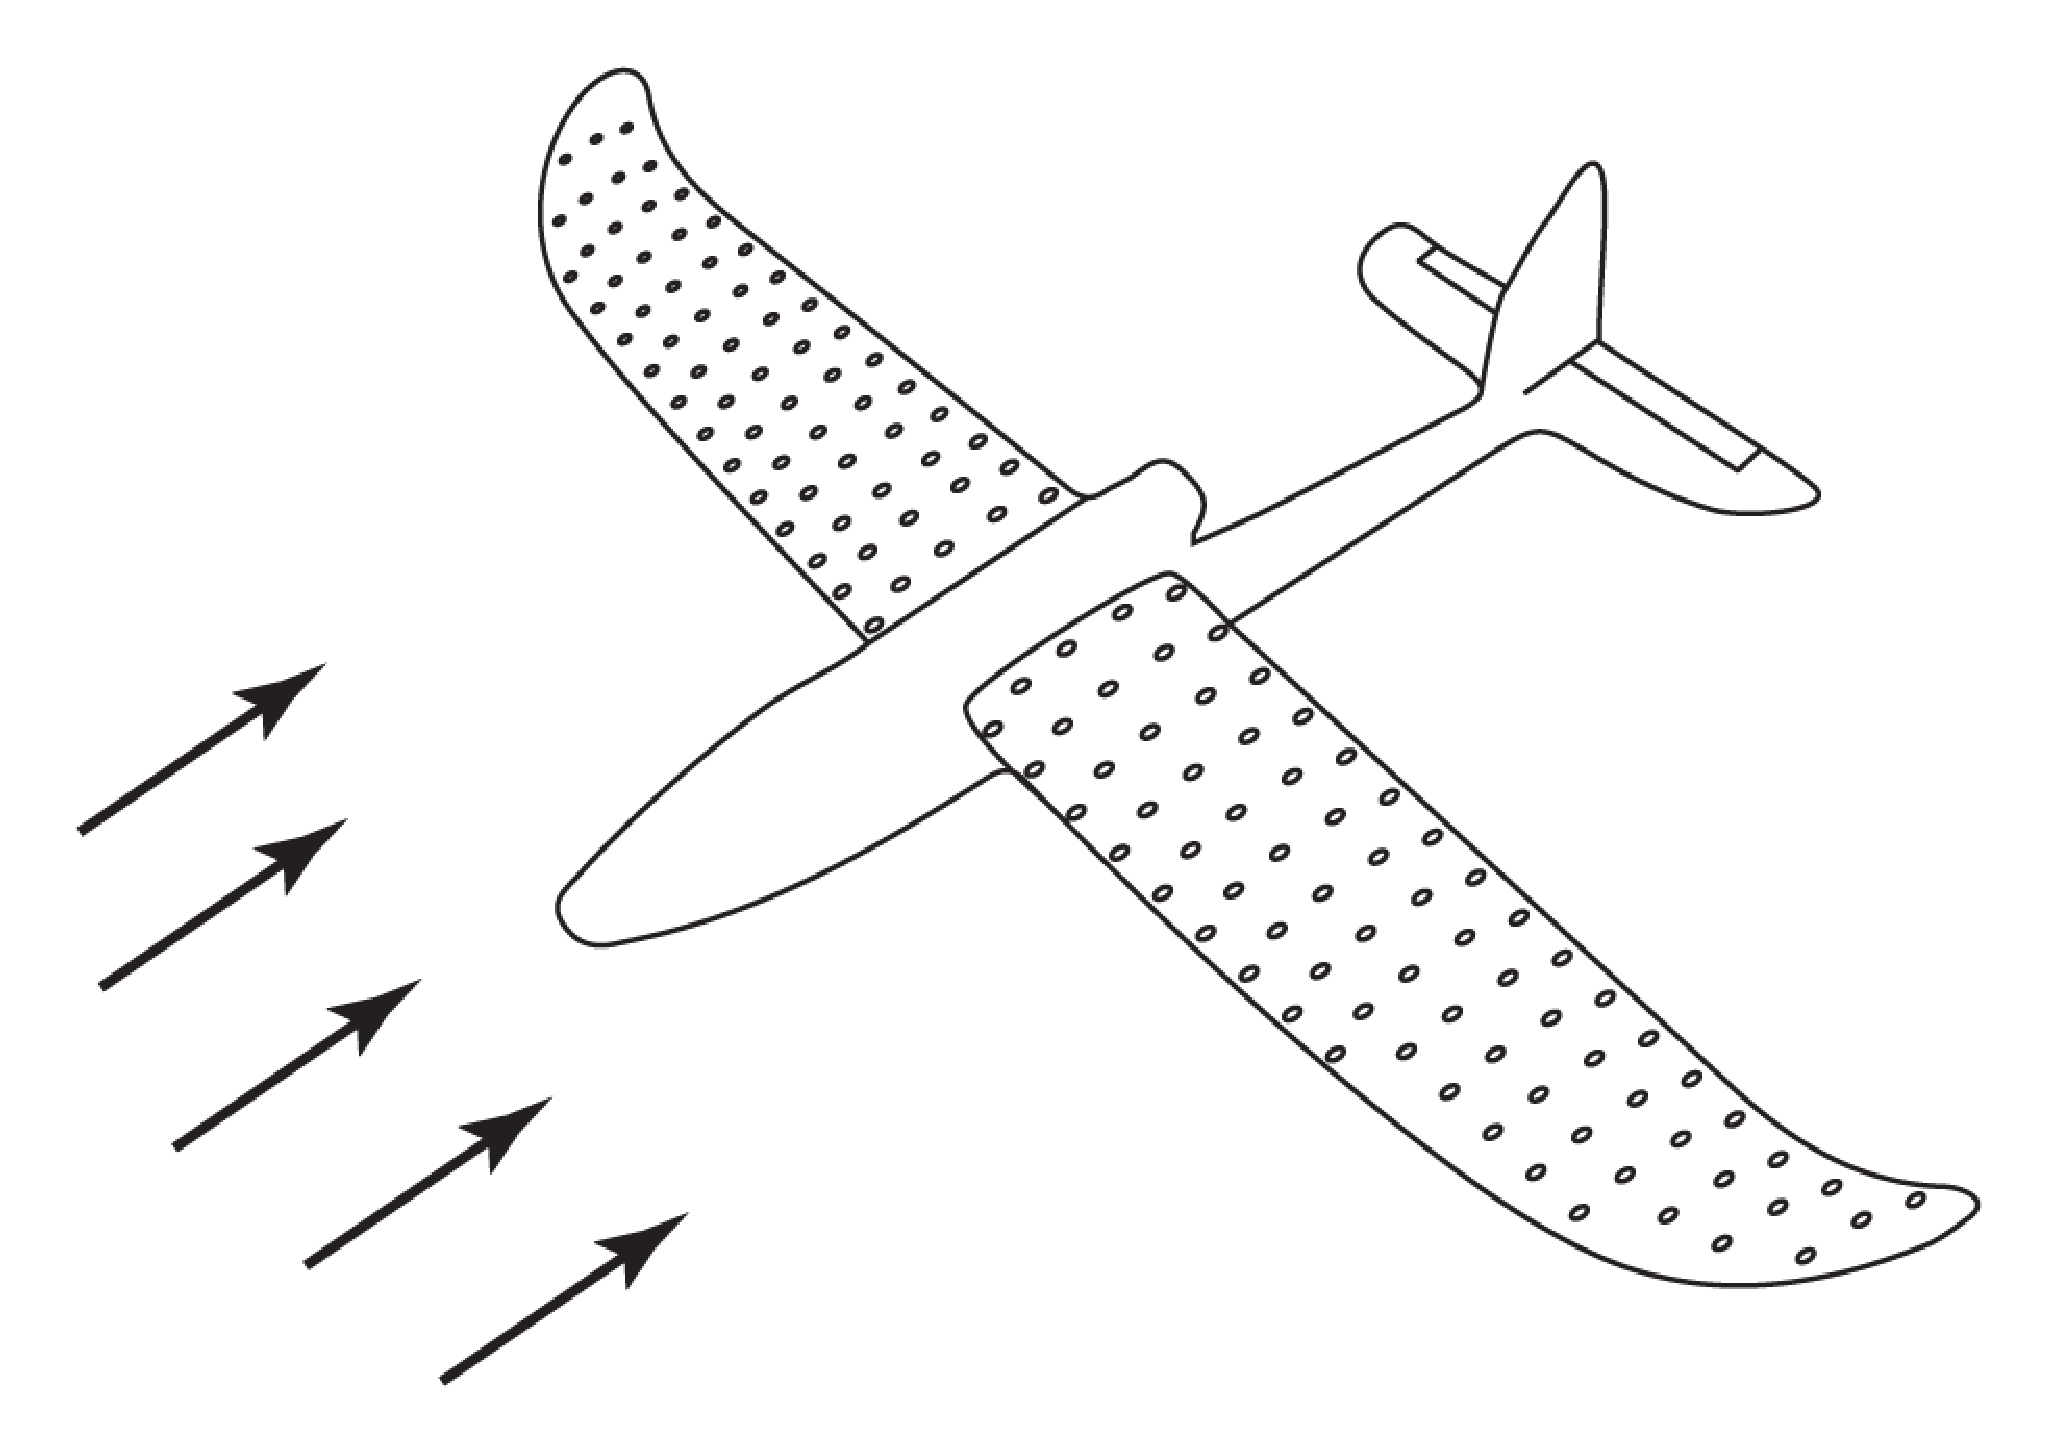
\includegraphics[height=0.45\textwidth]{DistSensingUAV.eps}
				\end{figure}
			}
		\end{column}
	\end{columns}
	
\end{frame}

%%%%%%%%%%%%%%%%%%%%%%%%%%%%%%%%%%%%%%%%%%%%%%%%%%%%%%%%%%%%%
%\begin{frame}{The hypothesis (or prediction)}
  %What do you think will happen?
  %
  %Fit strain \& differential pressure sensors
  %Carry out WT experiments
  %Carry out outdoors experiments
  %
  %\begin{itemize}
    %\item AoA, Windspeed aero loads compuation/prediction/estimation
    %\item Characterisation of pressure, strain \& force signals as function of ${\alpha}$, V
      %\& ${\delta_{ail}}$
    %\item Acquisition of training/testing daat sets for ANN for ${\alpha}$, V \&
      %${\delta_{ail}}$ prediction
    %\item Identification of stall characteristic markers in pressure \& strain signals, e.g.
      %frequency, variance
    %\item Acquisition of pressure \& strain characteristic response to change in ${q}$
    %\item Explore pressure \& strain response to conditions similar to perching manoeuvre\
    %\item Emulation of pressure \& strain response to gusts
    %\item Identify pressure \& strain response to varying ${q}$, i.e. ${\dot{q}}$
    %\item Vibration of wing has been observed during and after stall. How does this affect
      %pressure \& strain signals?
    %\item Identify pressure \& strain response to varying ${\delta_{ail}}$, i.e.
      %${\dot{\delta}_{ail}}$
  %\end{itemize}
%\end{frame}

%%%%%%%%%%%%%%%%%%%%%%%%%%%%%%%%%%%%%%%%%%%%%%%%%%%%%%%%%%%%
\section{Research at UoB}
\subsection[Previous Research]{Previous Research}
\begin{frame}{Previous Research at UoB: Strain sensing}

  \begin{columns}
    \begin{column}{0.6\textwidth}
		  \only<1>{		
				\begin{figure}[!htb]
	  			\centering
	  			\includegraphics[height=0.45\textwidth]{EasySkyGlider_WTGustTest.eps}
	  			\caption{Strain sensing platform}
	  			\label{Fig:StrainExpPlatform}
				\end{figure}
			}
			\only<2>{
			  \begin{figure}[!htb]
	  		  \centering
	  		  % StrainSensorsInWing.tex
\resizebox{!}{0.45\textwidth}{
	\begin{tikzpicture}
		% Auxiliary objects definition
		\tikzstyle{LabelObject}=[fill=white,rectangle,rounded corners,line width=0.5mm,%
			align=center]
		\tikzstyle{ArrowObject}=[red,line width=0.5mm, -latex]
		% Graphics display
	  \node[anchor=south west,inner sep=0] (image) at (0,0)%
	  {\includegraphics[width=\textwidth,trim= 50mm 0mm 50mm 0mm,clip,angle=180]%
	  	{StrainSensorsInWing.eps}};
	  % Define scope with 'image' dimensions as reference
	  \begin{scope}[x={(image.south east)},y={(image.north west)}]
%			  	\draw[help lines,xstep=.05,ystep=.05] (0,0) grid (1,1);
%			  	\foreach \x in {0,1,...,9} { \node [anchor=north] at (\x/10,0) {0.\x}; }
%			    \foreach \y in {0,1,...,9} { \node [anchor=east] at (0,\y/10) {0.\y}; }
	    %% Auxiliary coordinates
	    \coordinate (L0) at (0.875,0.41);   \coordinate (R0) at (0.050,0.42);
	    \coordinate (L1) at (0.800,0.42);   \coordinate (R1) at (0.125,0.41);
	    \coordinate (L2) at (0.720,0.41);   \coordinate (R2) at (0.200,0.42);
	    \coordinate (L3) at (0.640,0.42);   \coordinate (R3) at (0.280,0.41);
	    \coordinate (L4) at (0.565,0.41);   \coordinate (R4) at (0.360,0.42);
	    \coordinate (L5) at (0.490,0.42);   \coordinate (R5) at (0.440,0.41);
	    %% Labels
	    \draw(0.875,0.25) node[LabelObject] (L0_Label) {${L0}$};
	    \draw(0.800,0.55) node[LabelObject] (L1_Label) {${L1}$};
	    \draw(0.720,0.25) node[LabelObject] (L2_Label) {${L2}$};
	    \draw(0.640,0.55) node[LabelObject] (L3_Label) {${L3}$};
	    \draw(0.565,0.25) node[LabelObject] (L4_Label) {${L4}$};
	    \draw(0.490,0.55) node[LabelObject] (L5_Label) {${L5}$};
	    \draw(0.440,0.25) node[LabelObject] (R5_Label) {${R5}$};
	    \draw(0.360,0.55) node[LabelObject] (R4_Label) {${R4}$};
	    \draw(0.280,0.25) node[LabelObject] (R3_Label) {${R3}$};
	    \draw(0.200,0.55) node[LabelObject] (R2_Label) {${R2}$};
	    \draw(0.125,0.25) node[LabelObject] (R1_Label) {${R1}$};
	    \draw(0.050,0.55) node[LabelObject] (R0_Label) {${R0}$};
	    %% Arrows
			\draw[ArrowObject] (L0_Label.north) -- (L0);
			\draw[ArrowObject] (L1_Label.south) -- (L1);
			\draw[ArrowObject] (L2_Label.north) -- (L2);
			\draw[ArrowObject] (L3_Label.south) -- (L3);
			\draw[ArrowObject] (L4_Label.north) -- (L4);
			\draw[ArrowObject] (L5_Label.south) -- (L5);
			\draw[ArrowObject] (R5_Label.north) -- (R5);
			\draw[ArrowObject] (R4_Label.south) -- (R4);
			\draw[ArrowObject] (R3_Label.north) -- (R3);
			\draw[ArrowObject] (R2_Label.south) -- (R2);
			\draw[ArrowObject] (R1_Label.north) -- (R1);
			\draw[ArrowObject] (R0_Label.south) -- (R0);
	  \end{scope}
	\end{tikzpicture}
}
	  		  \caption{Strain sensing platform instrumentation}
	  		  \label{Fig:StrainExpPlatformInst}
			  \end{figure}
			}
			\only<3>{		
				\begin{figure}[!htb]
	  			\centering
	  			% StrainWTDataSet_RightWing.tex

\resizebox{!}{0.45\textwidth}{
	\begin{tikzpicture}
		\node[anchor=south west,inner sep=0] (image) at (0,0)%
			{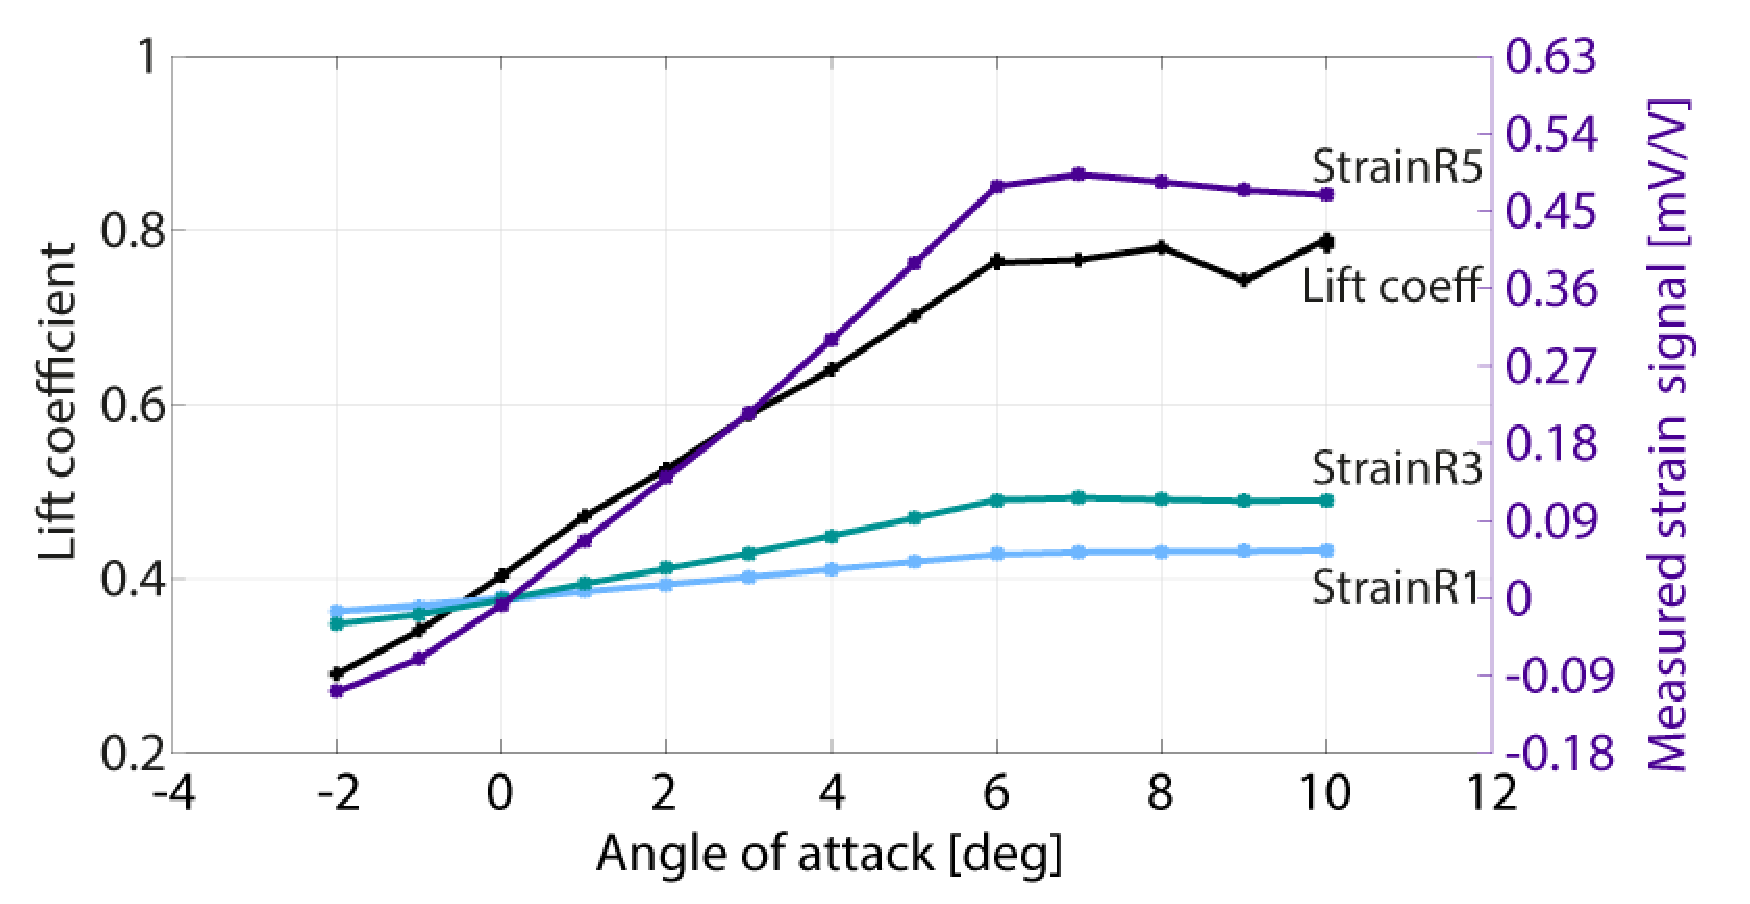
\includegraphics[width=\textwidth]{StrainWTDataSet_RightWing.eps}};
		% Define scope with 'image' dimensions as reference
		\begin{scope}[x={(image.south east)},y={(image.north west)}]
			\draw[help lines,xstep=.05,ystep=.05] (0,0) grid (1,1);
			\foreach \x in {0,1,...,9} { \node [anchor=north] at (\x/10,0) {0.\x}; }
			\foreach \y in {0,1,...,9} { \node [anchor=east] at (0,\y/10) {0.\y}; }
			
		\end{scope}
  \end{tikzpicture}
}
	  			\caption{Strain wind tunnel characterisation}
	  			\label{Fig:StrainWTChar}
				\end{figure}
			}
		\end{column}
		\begin{column}{0.4\textwidth}
			\begin{itemize}
				\item<2-> 12 full-bridge strain gauges and amplifiers distributed along spar of wing
				\item<3-> Wind tunnel characterisation
			\end{itemize}
		\end{column}
	\end{columns}

\end{frame}

%%%%%%%%%%%%%%%%%%%%%%%%%%%%%%%%%%%%%%%%%%%%%%%%%%%%%%%%%%%%
\begin{frame}{Previous Research at UoB: Strain sensing}

  \begin{columns}
    \begin{column}{0.6\textwidth}
			\only<-4>{
			  \begin{figure}[!htb]
	  		  \centering
	  		  \includegraphics[height=0.45\textwidth]{EasySkyGlider_WTGustTest.eps}
	  		  \caption{Strain sensing platform}
	  	    \label{Fig:StrainExpPlatform2}
			  \end{figure}
			}
			\only<5->{
			  \begin{figure}[!htb]
	  			\centering
	  			% Strain_OutdoorsResponse2Controls.tex

\tikzstyle{RectObject}=[rectangle,draw=blue,rounded corners,line width=0.5mm,
  minimum width=21em,minimum height=8em]
\tikzstyle{LabelObject}=[fill=white,rectangle,rounded corners,line width=0.5mm,%
	align=center]
\tikzstyle{ArrowObject}=[red,line width=1.0mm, -latex]

\resizebox{!}{0.45\textwidth}{
	\begin{tikzpicture}
		\node[anchor=south west,inner sep=0] (image) at (0,0)%
			{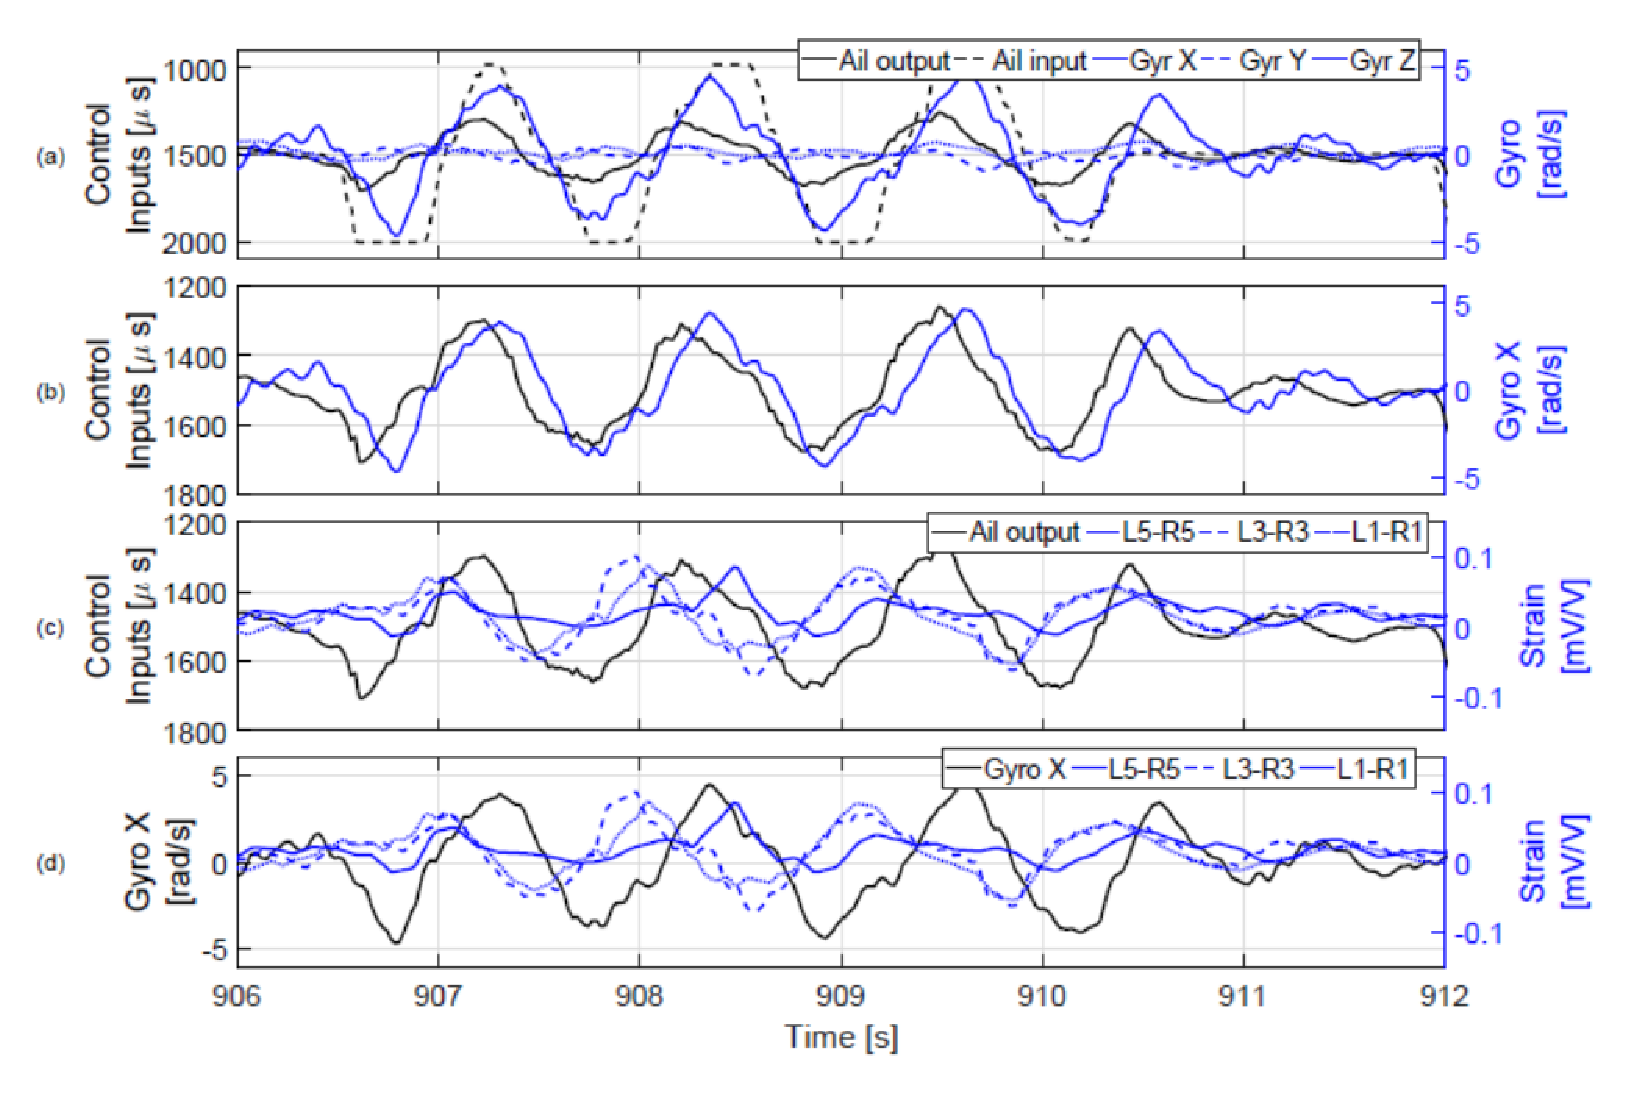
\includegraphics[width=\textwidth]{Strain_OutdoorsResponse2Controls.eps}};
		% Define scope with 'image' dimensions as reference
		\begin{scope}[x={(image.south east)},y={(image.north west)}]
			%\draw[help lines,xstep=.05,ystep=.05] (0,0) grid (1,1);
			%\foreach \x in {0,1,...,9} { \node [anchor=north] at (\x/10,0) {0.\x}; }
			%\foreach \y in {0,1,...,9} { \node [anchor=east] at (0,\y/10) {0.\y}; }
			
			\only<6>{
			  % Gyro Response
			  \draw(0.515,0.75) node[RectObject] (GyroResponse) {};
			  % Gyro Response label
			  \draw(0.515,0.30) node[LabelObject] (GyroResponse_Label)
				  {Gyro Response\\ to Aileron Command};
			  % Gyro Response arrow
			  \draw[ArrowObject] (GyroResponse_Label.north) -- (GyroResponse.south);
			}
			\only<7>{
			  % Gyro Response
			  \draw(0.515,0.315) node[RectObject] (StrainResponse) {};
			  % Gyro Response label
			  \draw(0.515,0.85) node[LabelObject] (StrainResponse_Label)
				  {Strain Response\\ to Aileron Command};
			  % Gyro Response arrow
			  \draw[ArrowObject] (StrainResponse_Label.south) -- (StrainResponse.north);
			}
			
		\end{scope}
  \end{tikzpicture}
}
	  			\caption{Strain response to control inputs}
	  			\label{Fig:Strain_OutdoorsResponse2Controls}
				\end{figure}
			}
		\end{column}
		\begin{column}{0.4\textwidth}
			\begin{itemize}
			  \item<2-> {\movie[width=0.8\textwidth,externalviewer]{Response to controlled gusts}
					{./Videos/Strain_WTGust.mp4}}
				\item<3-> {\movie[width=0.8\textwidth,externalviewer]{Open loop free flight}
					{./Videos/StrainSensingExperiment_037_SlowDownShort.mp4}}
				\item<4-> {\movie[width=0.8\textwidth,externalviewer]{Closed loop free flight}
					{./Videos/StrainFeedbackCtrl_GustRejection.mp4}}
				\item<5-> Outdoor flight testing
			\end{itemize}
		\end{column}
	\end{columns}

  \note[item]<2>{Click on 'Response to controlled gusts' to show gust video:}
	\note[item]<3>{Click on 'Open loop free flight' to show open-loop video}
	\note[item]<4>{Click on 'Closed loop free flight' to show closed-loop video}
	\note[item]<5>{Outdoor flight graph}

\end{frame}

%%%%%%%%%%%%%%%%%%%%%%%%%%%%%%%%%%%%%%%%%%%%%%%%%%%%%%%%%%%%
\begin{frame}{Previous Research at UoB: Pressure sensing}

  \begin{columns}
    \begin{column}{0.6\textwidth}
		  \only<1,5>{
        \begin{figure}[!htb]
			    \centering
          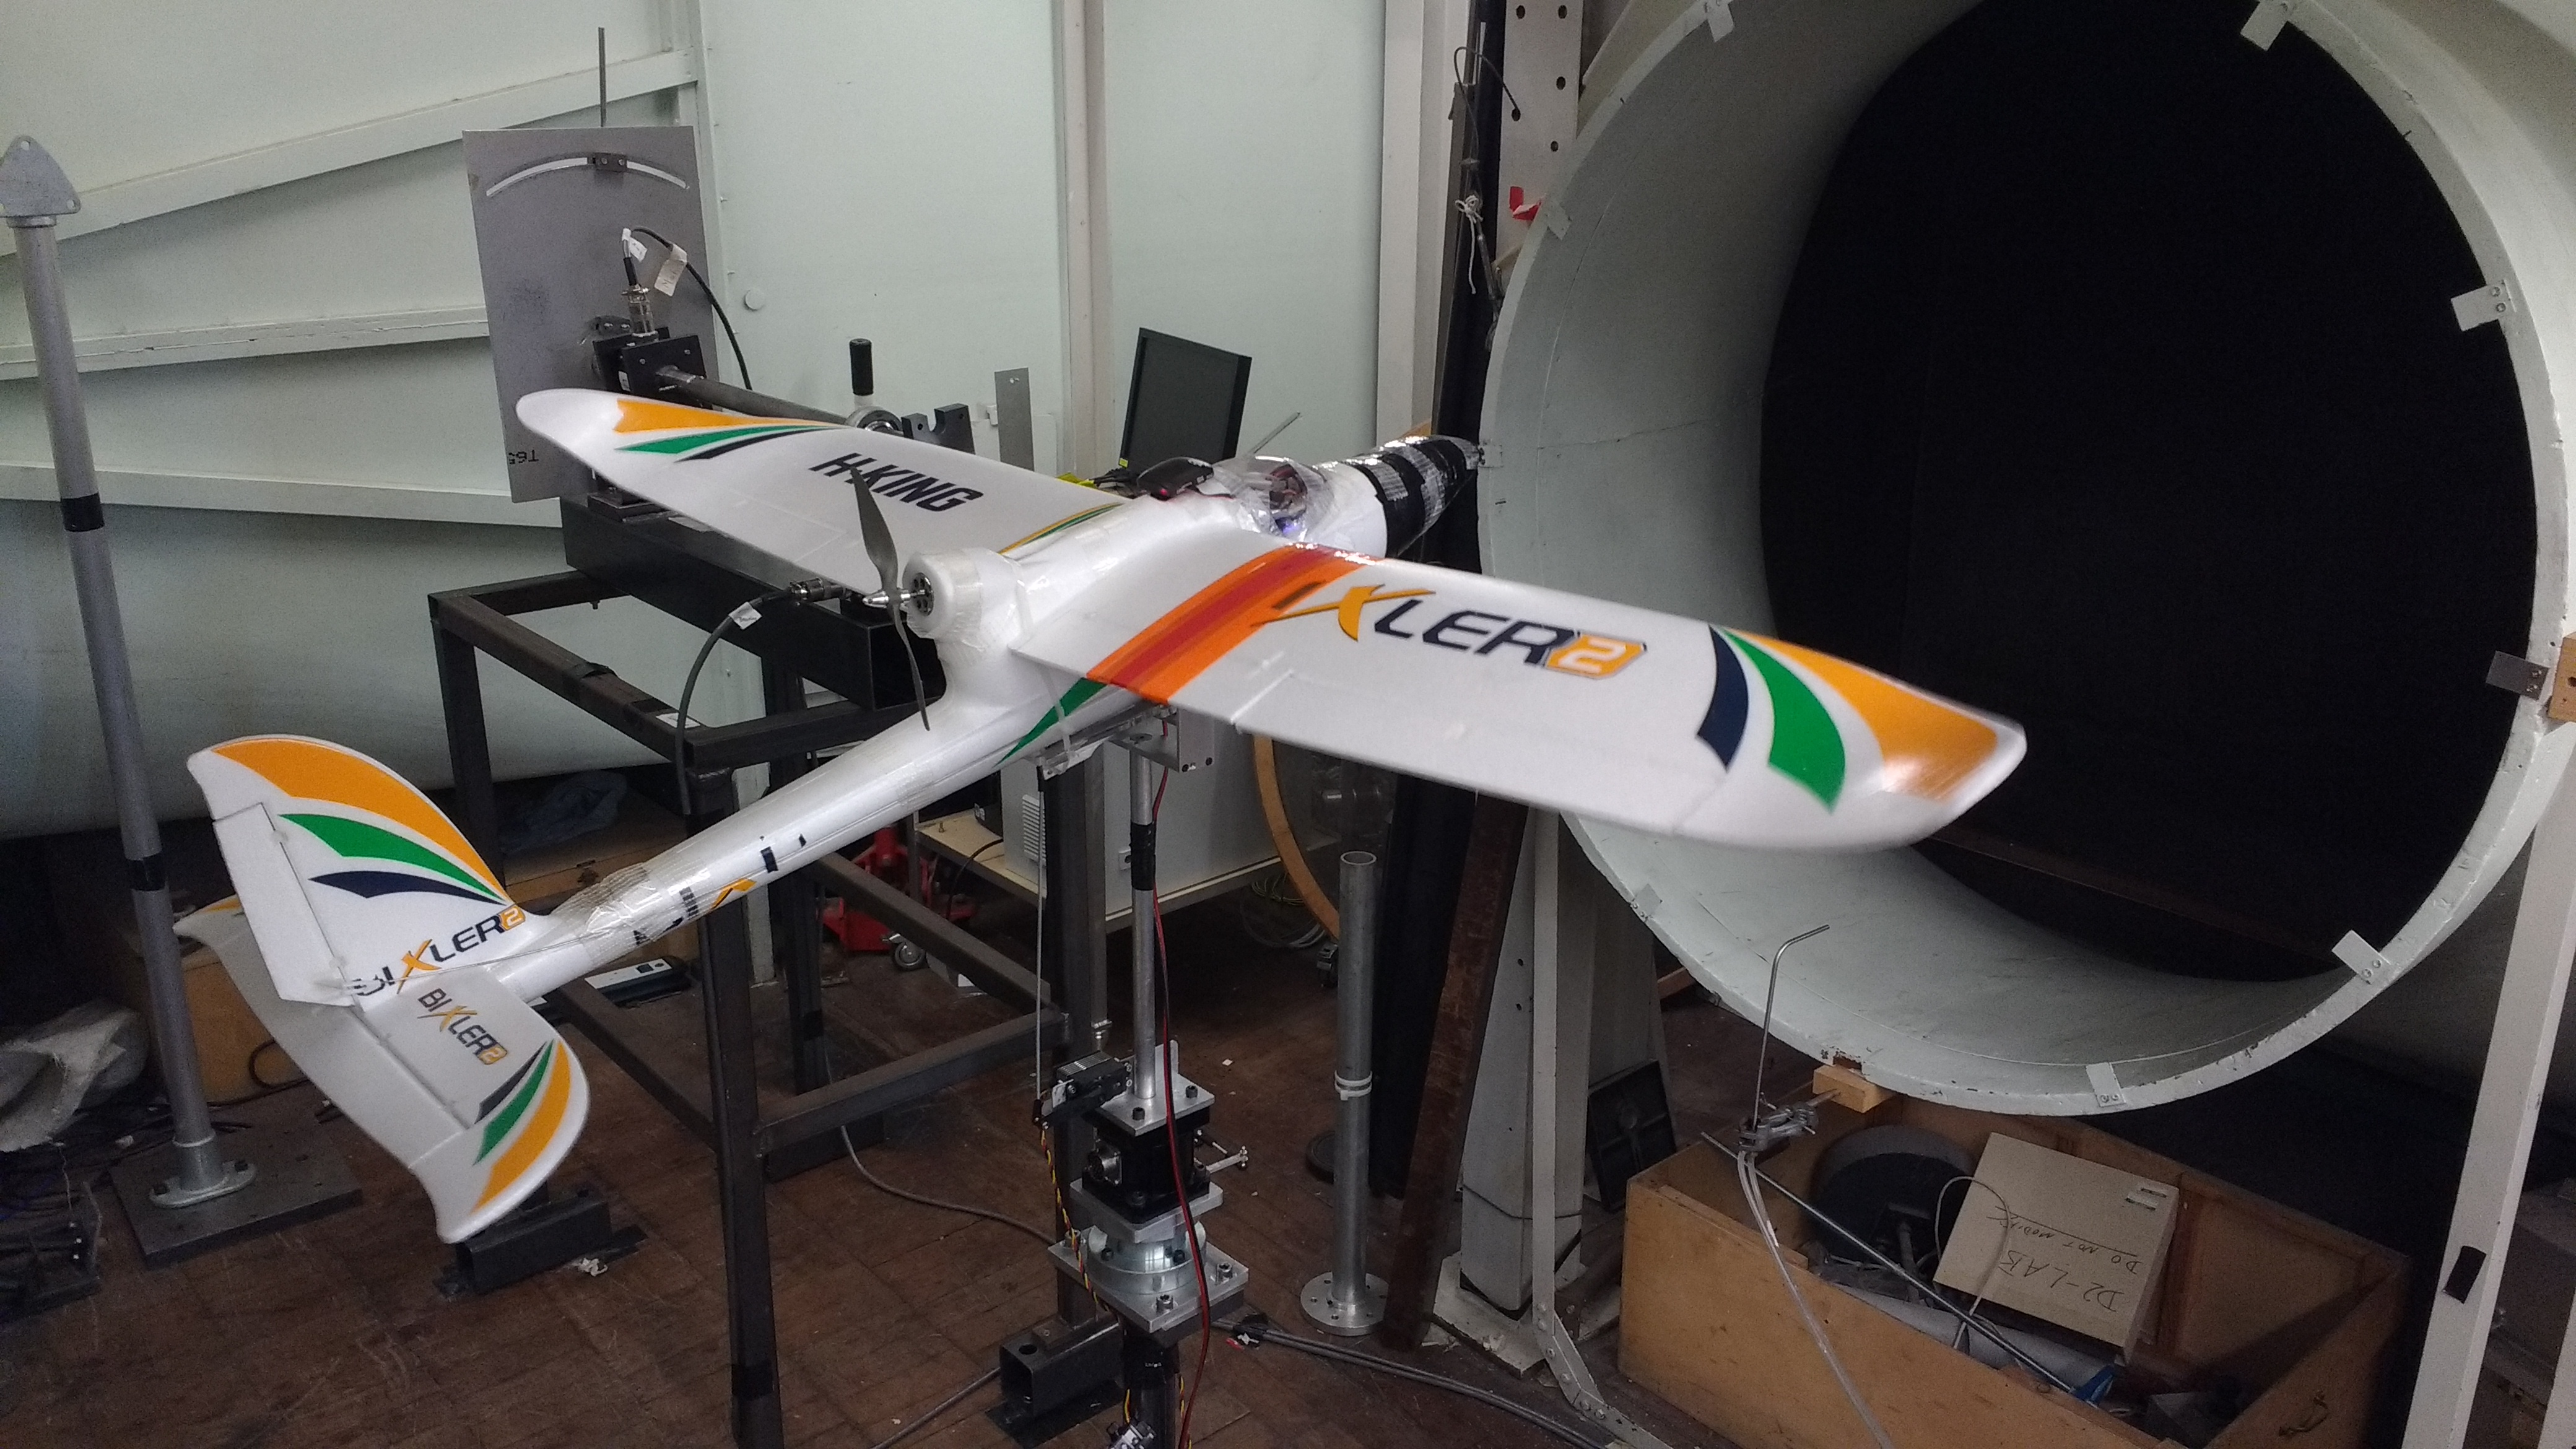
\includegraphics[height=0.45\textwidth]{Bixler_WTTest.eps}
          \caption{Pressure sensing platform}
          \label{Fig:PressureExpPlatform}
        \end{figure}
      }
		  \only<2>{
        \begin{figure}[!htb]
			    \centering
					% PressureExpPlatform_3DInsert.tex

\tikzstyle{RectObject}=[rectangle,draw=blue,,rounded corners,line width=0.5mm,minimum width=4.0em,%
	minimum height=1em]
\tikzstyle{LabelObject}=[fill=white,rectangle,rounded corners,line width=0.5mm,%
	align=center]
\tikzstyle{ArrowObject}=[red,line width=1.0mm, -latex]

\resizebox{!}{0.45\textwidth}{
  \begin{tikzpicture}
    \node[anchor=south west,inner sep=0] (image) at (0,0)%
		  {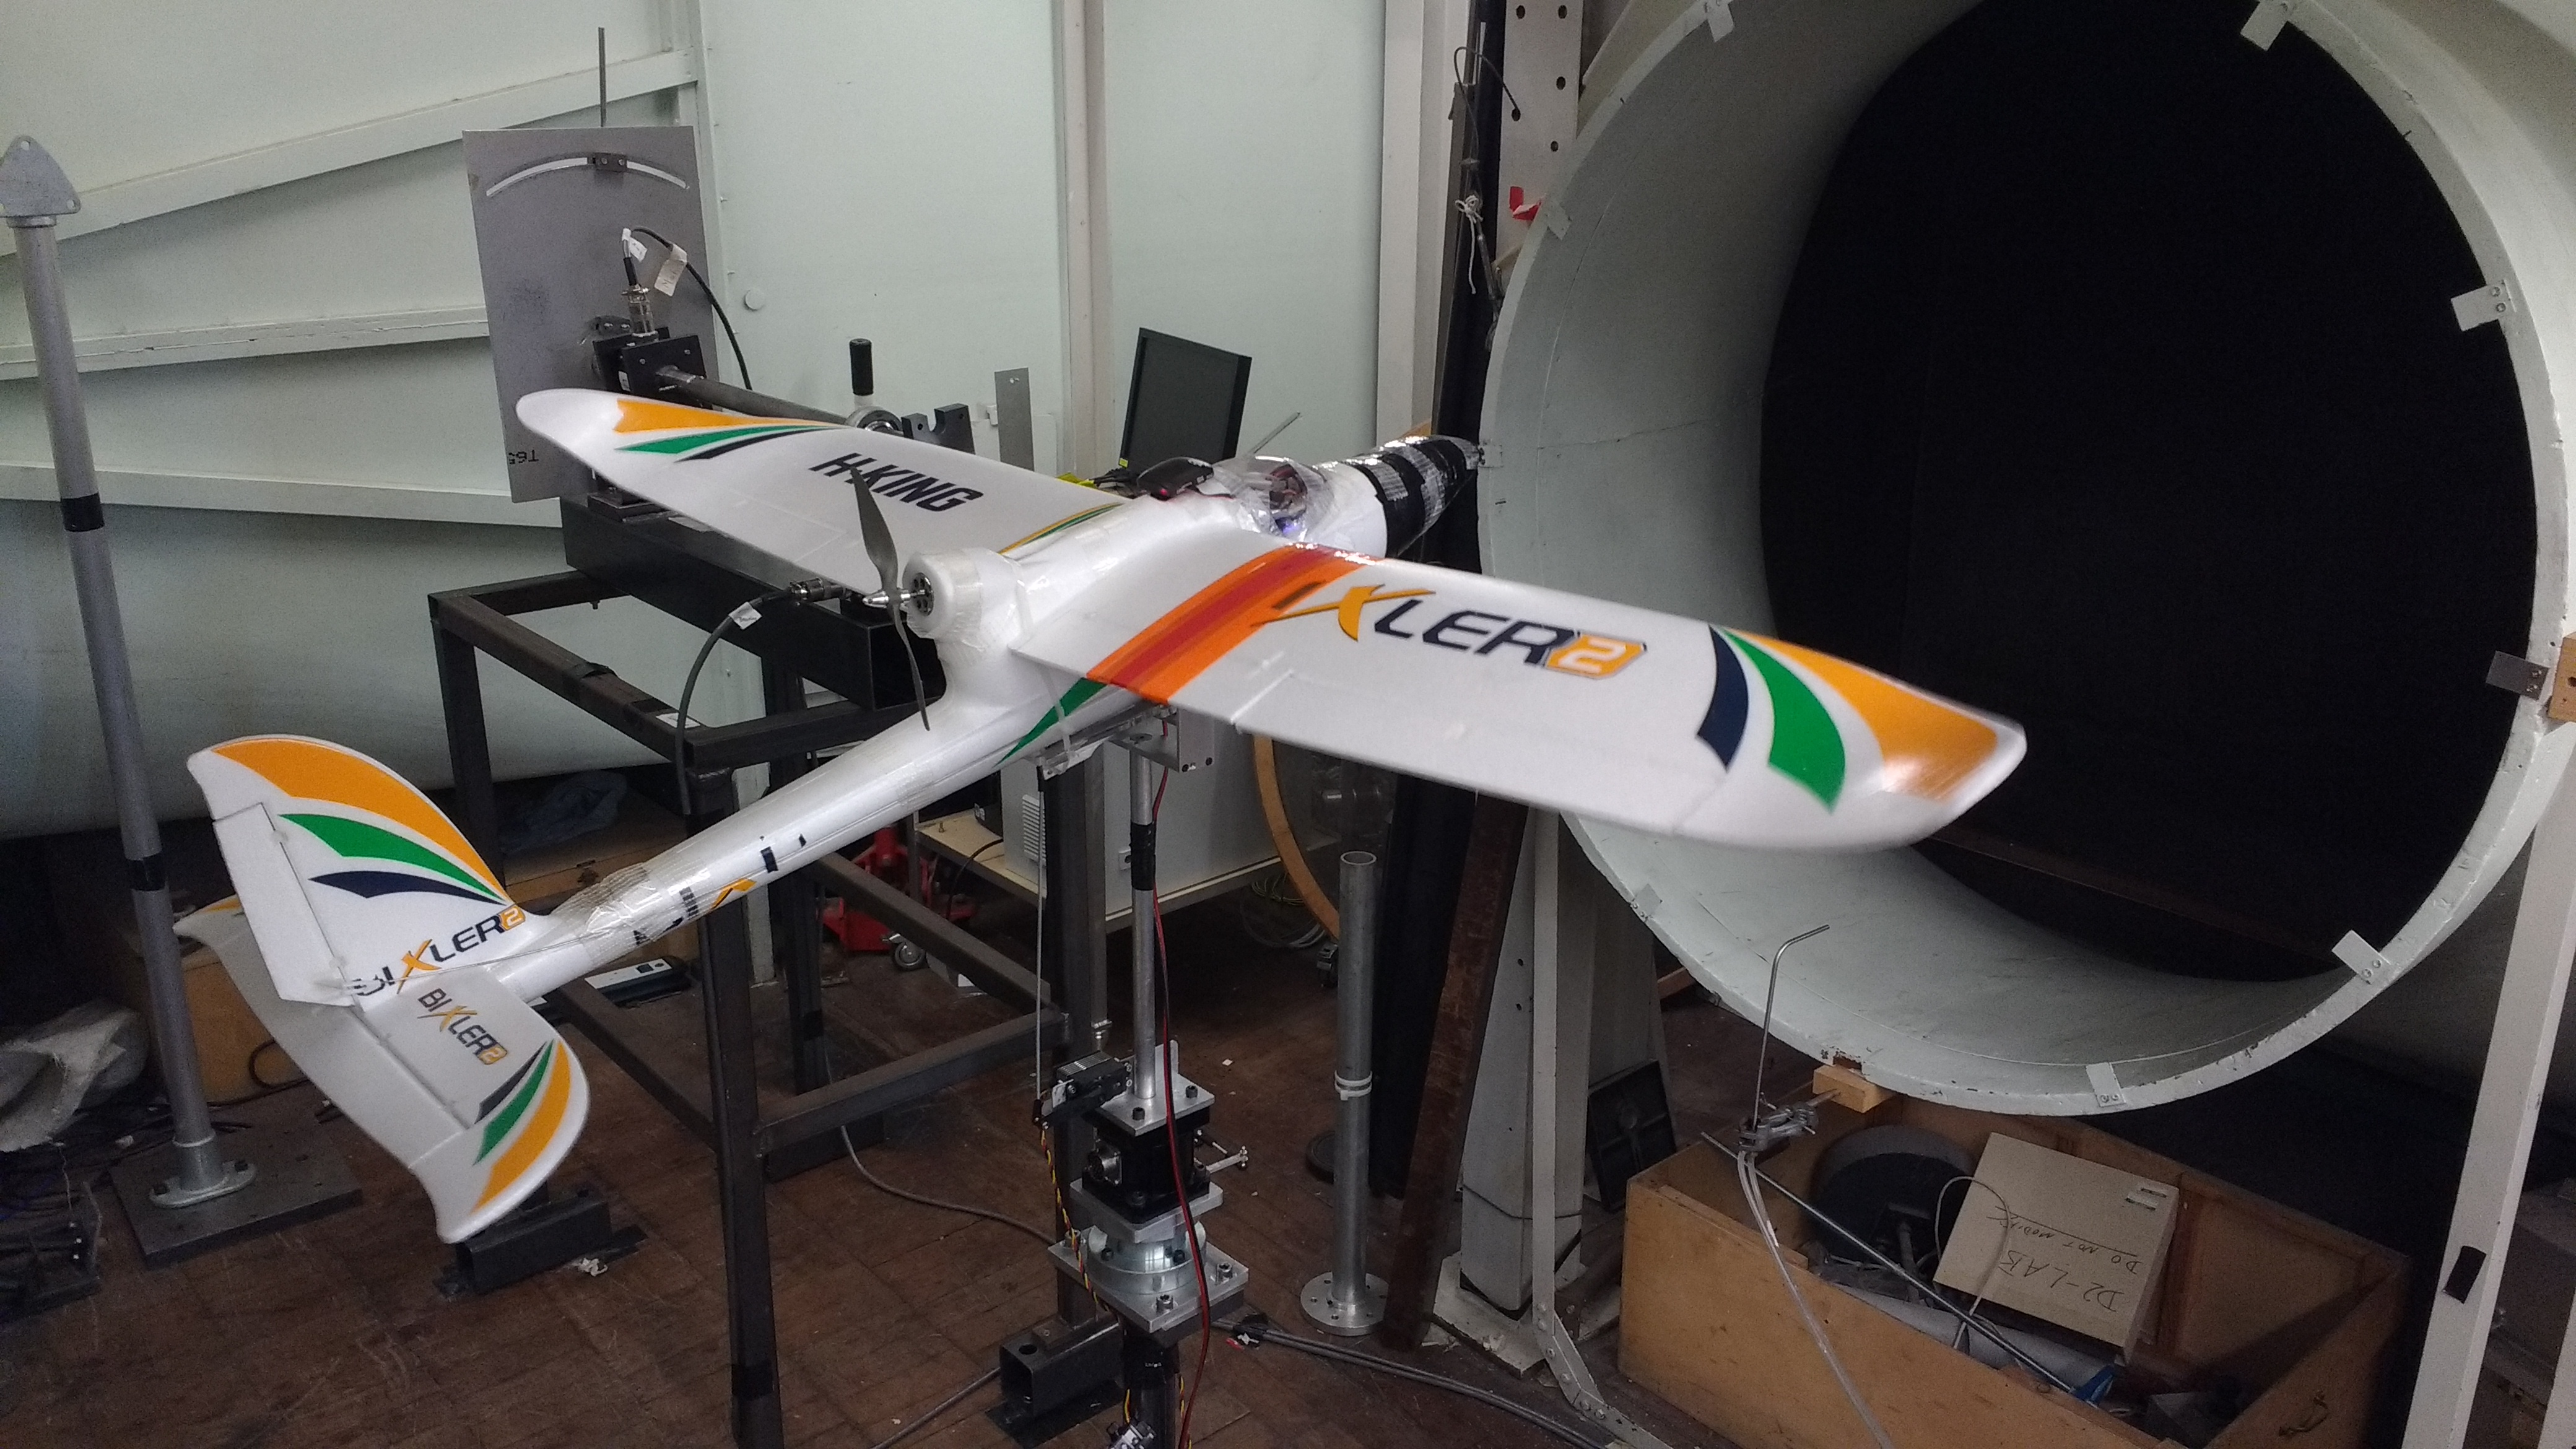
\includegraphics[width=\textwidth]{Bixler_WTTest.eps}};
    % Define scope with 'image' dimensions as reference
    \begin{scope}[x={(image.south east)},y={(image.north west)}]
      \draw[help lines,xstep=.05,ystep=.05] (0,0) grid (1,1);
      \foreach \x in {0,1,...,9} { \node [anchor=north] at (\x/10,0) {0.\x}; }
      \foreach \y in {0,1,...,9} { \node [anchor=east] at (0,\y/10) {0.\y}; }
			
			% Servo Elements
			\draw(0.475,0.575) node[RectObject,rotate around={35:(0,0)}] (WingInsert) {};
			% Servo Labels
			\draw(0.85,0.85) node[LabelObject] (WingInsert_Label) {3-D Printed\\Insert};
			% Servo Arrows
			\draw[ArrowObject] (WingInsert_Label.west) -- (WingInsert.east);
			
    \end{scope}
  \end{tikzpicture}
}
          \caption{Pressure sensing platform}
          \label{Fig:PressureExpPlatform_3DInsert}
        \end{figure}
      }
      \only<3>{
        \begin{figure}[!htb]
          \centering
          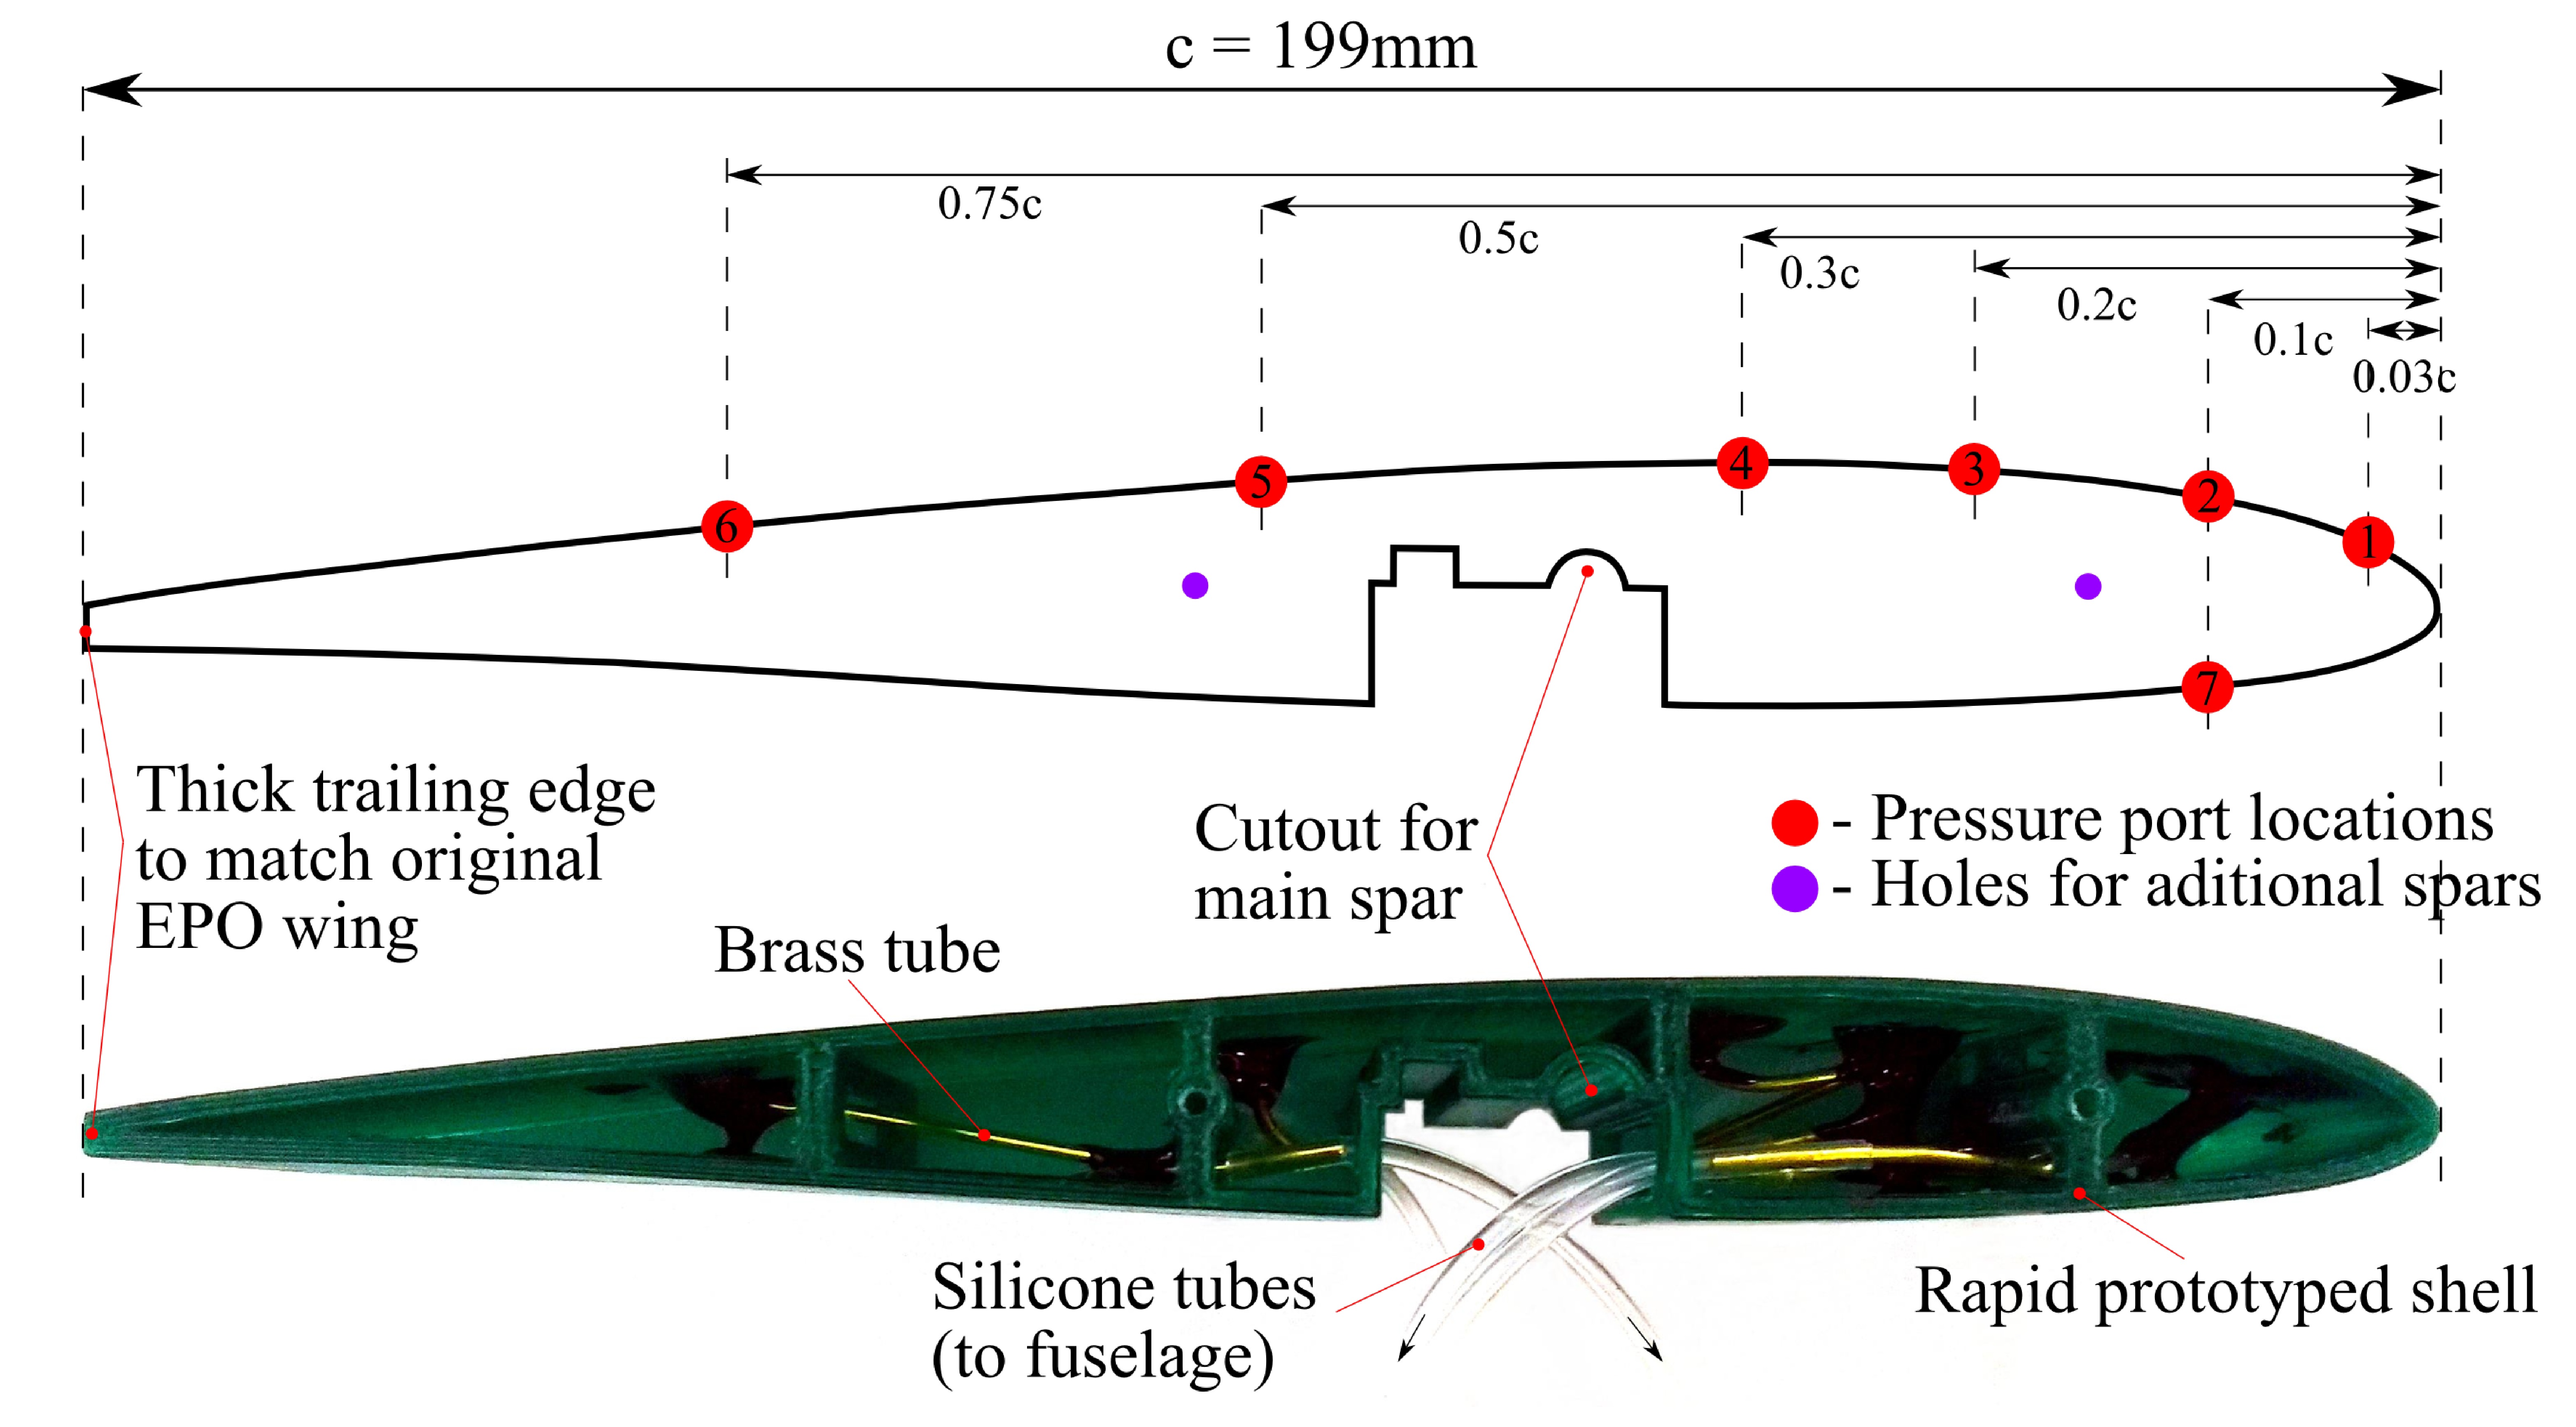
\includegraphics[height=0.45\textwidth]{wingInsertDiagram.eps}
          \caption{Pressure sensing platform instrumentation}
          \label{Fig:PressureExpPlatformInst}
        \end{figure}
      }
			\only<4>{
        \begin{figure}[!htb]
          \centering
	  			% PressureWTChar.tex

\resizebox{!}{0.45\textwidth}{
	\begin{tikzpicture}
		\node[anchor=south west,inner sep=0] (image) at (0,0)%
			{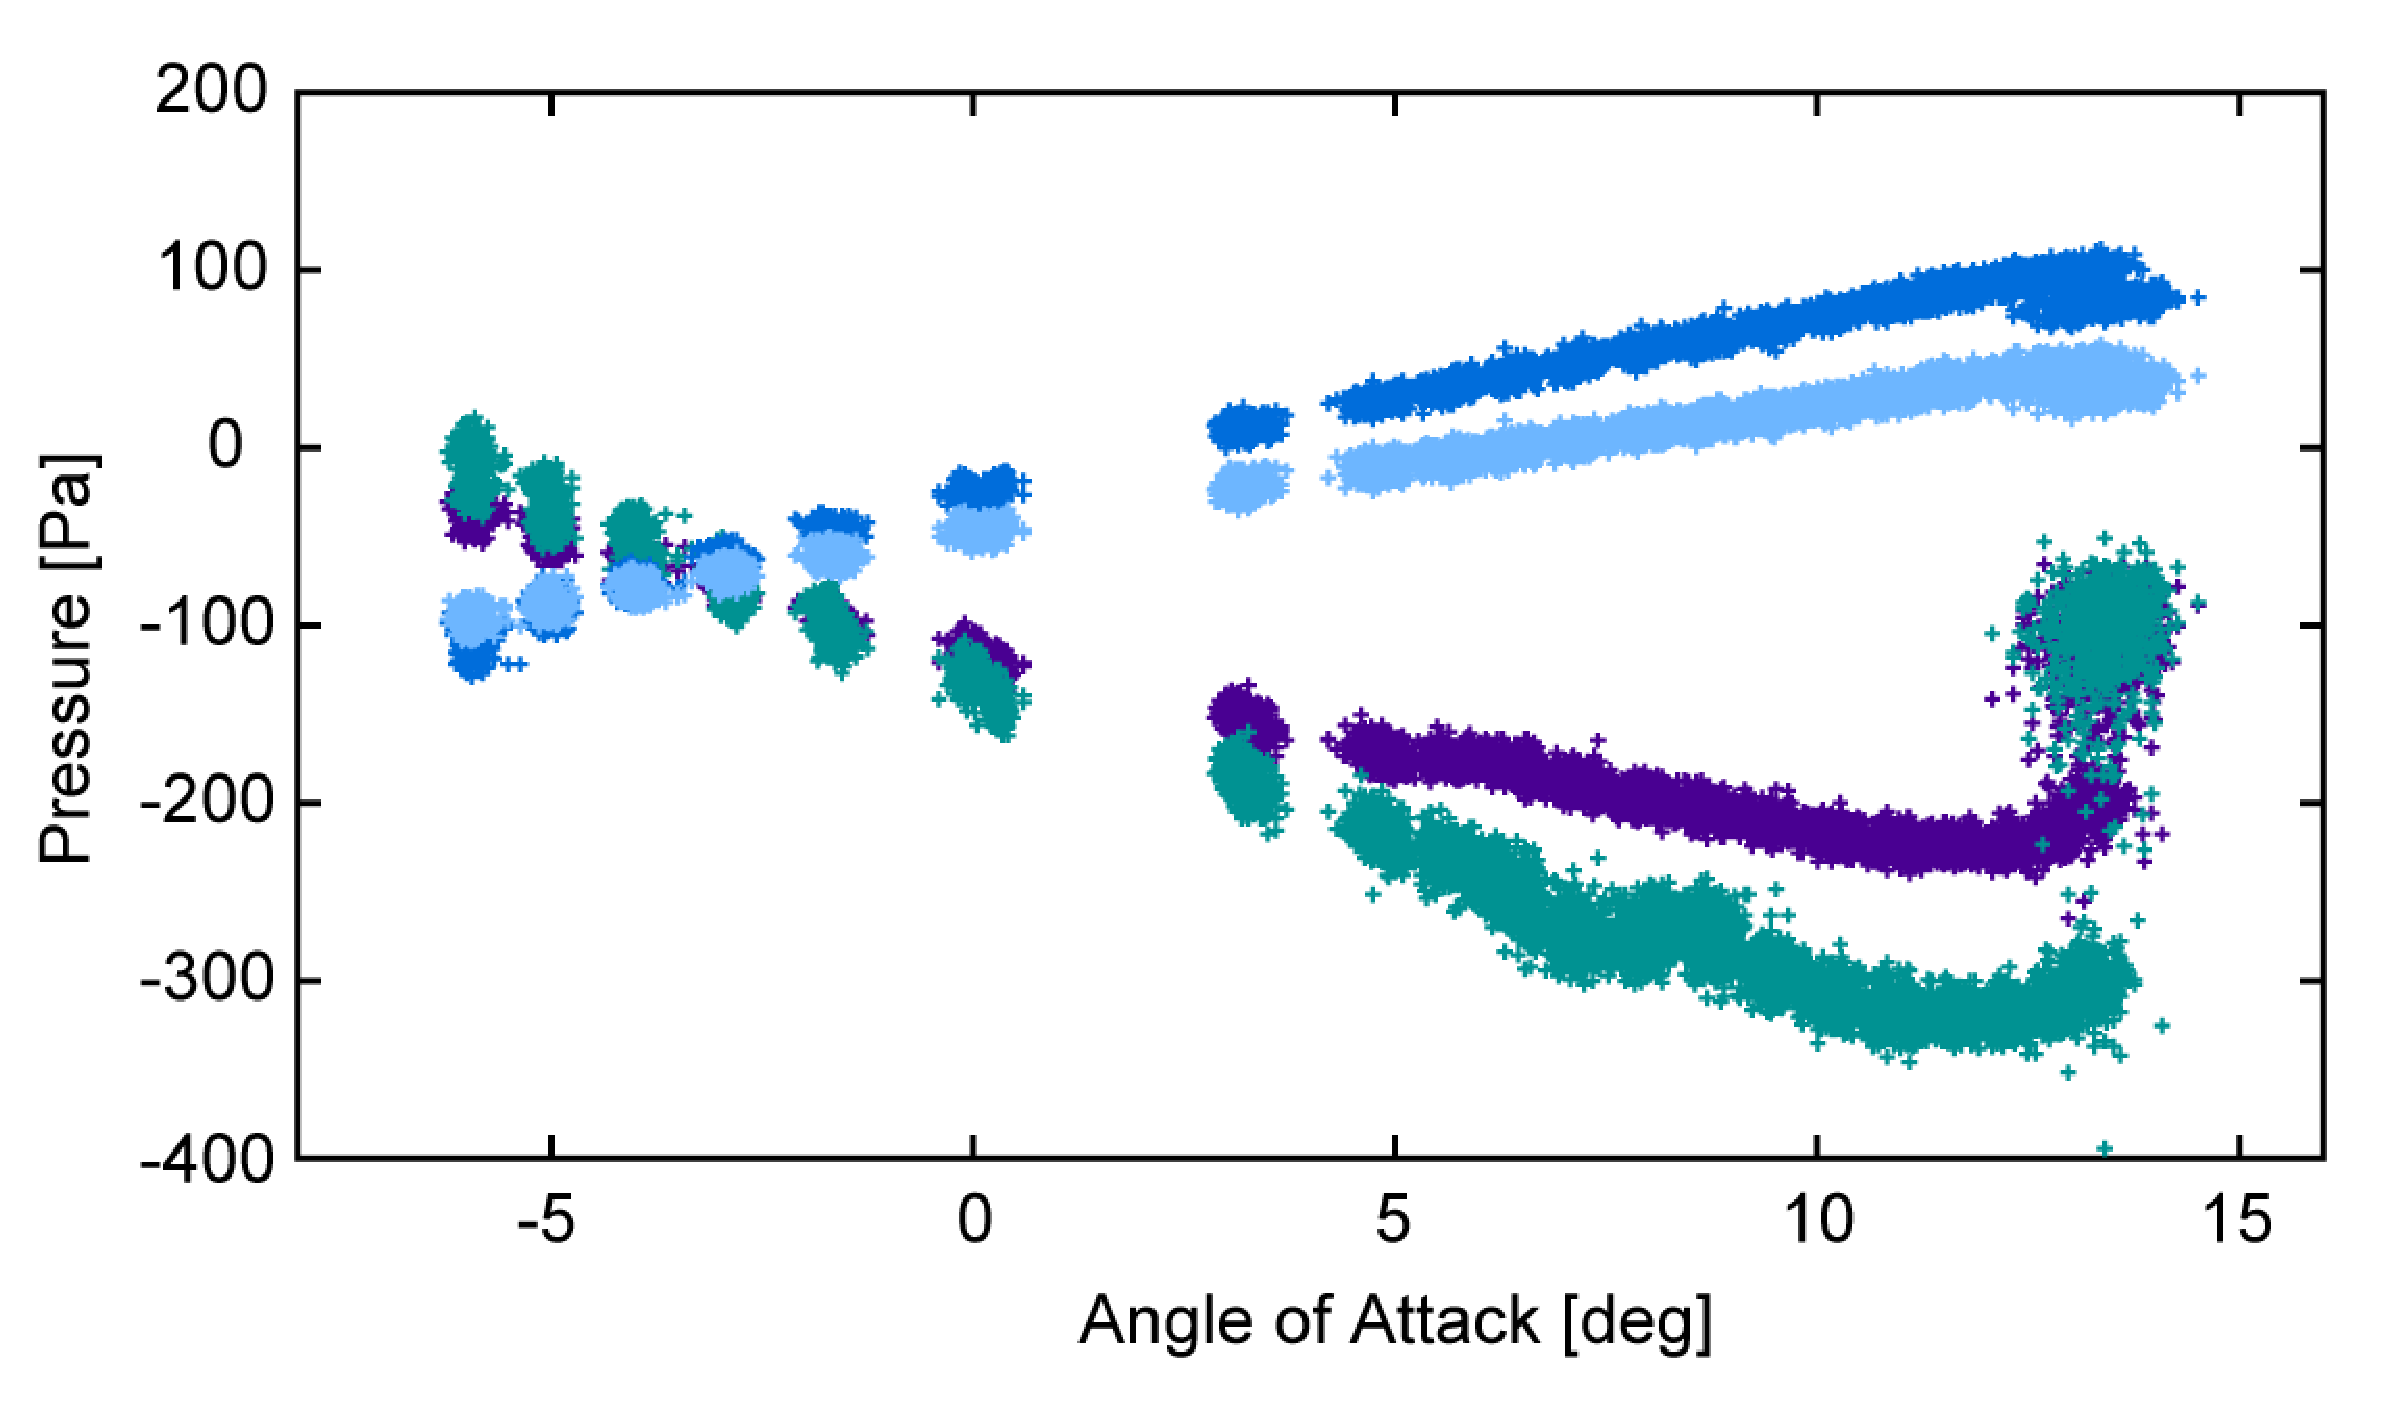
\includegraphics[width=\textwidth]{Flow-pressure-vs-AoA-no-lines.eps}};
		% Define scope with 'image' dimensions as reference
		\begin{scope}[x={(image.south east)},y={(image.north west)}]
			\draw[help lines,xstep=.05,ystep=.05] (0,0) grid (1,1);
			\foreach \x in {0,1,...,9} { \node [anchor=north] at (\x/10,0) {0.\x}; }
			\foreach \y in {0,1,...,9} { \node [anchor=east] at (0,\y/10) {0.\y}; }
			
		\end{scope}
  \end{tikzpicture}
}
          \caption{Pressure wind tunnel characterisation}
          \label{Fig:PressureWTChar}
        \end{figure}
      }
			\only<6>{
        \begin{figure}[!htb]
          \centering
          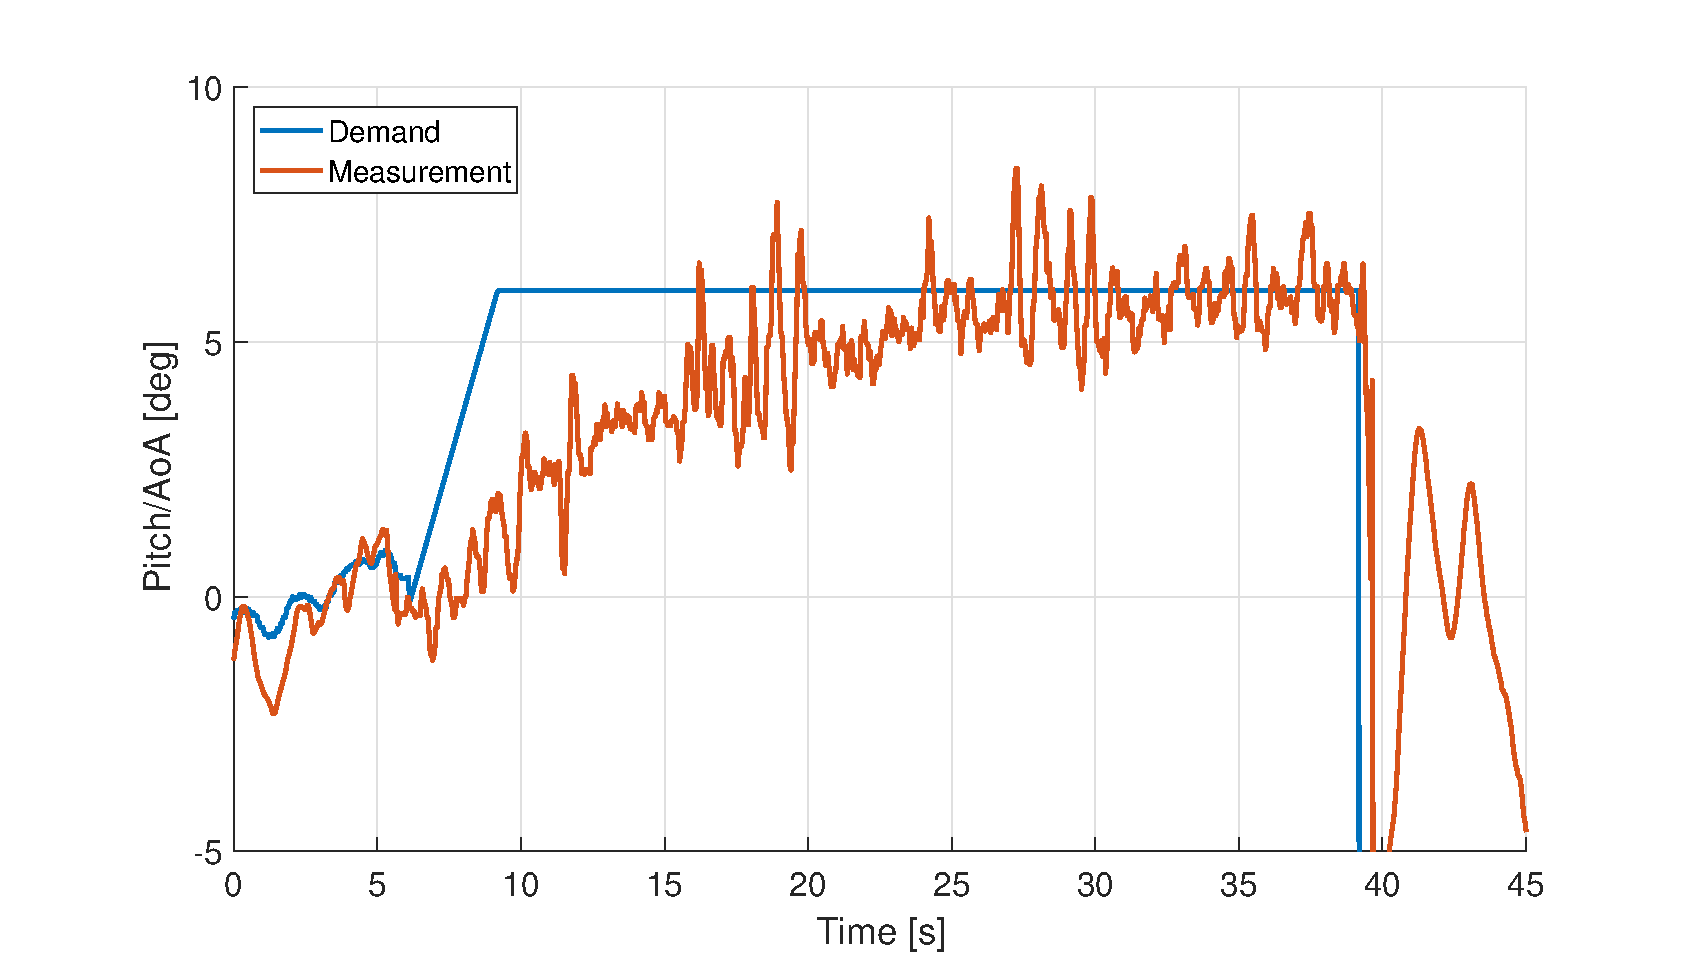
\includegraphics[height=0.45\textwidth]{PressSens_AoATracking.eps}
          \caption{outdoors angle-of-attack tracking}
          \label{Fig:PressSens_AoATracking}
        \end{figure}
			}
		\end{column}
		\begin{column}{0.4\textwidth}
		  \begin{itemize}
				\item<2-> 3-D printed insert on starboard wing
				\item<3-> 7 static-pressure ports distributed along wing-chord
				\item<4-> Wind tunnel characterisation
				\item<5-> \movie[width=0.8\textwidth,externalviewer]{%
				  Closed loop 1DOF WT testing}
					{./Videos/WTAoATracking.mp4}
				\item<6-> Outdoor flight testing
			\end{itemize}
		\end{column}
  \end{columns}
	
\end{frame}

%%%%%%%%%%%%%%%%%%%%%%%%%%%%%%%%%%%%%%%%%%%%%%%%%%%%%%%%%%%%
\begin{frame}{Previous Research at UoB: Pressure sensing}
  What did we learned?
	\pause
    \begin{itemize}[<+->]
      \item Strain \& pressure signal show
			\begin{itemize}[<+->]
			  \item[-]Linear response with AoA
			  \item[-]Stall markers
			\end{itemize}
			\item Similar performance to IMU-based control
			\begin{itemize}[<+->]
			  \item[-]Strain ${\rightarrow}$ roll control
        \item[-]Pressure ${\rightarrow}$ pitch control
			\end{itemize}
			\item Information not available using IMU: AoA, stall, roll acceleration, non-linear lift
    \end{itemize}
\end{frame}

%%%%%%%%%%%%%%%%%%%%%%%%%%%%%%%%%%%%%%%%%%%%%%%%%%%%%%%%%%%%
\subsection[Current Research]{Current Research}

\begin{frame}{Current Research at UoB}

  Research focuses on:
  \pause
	\begin{itemize}[<+->]
    \item Pressure and strain sensing experimental platform
    \item Calibration \& characterisation experiments
    \item Closed loop control algorithms
  \end{itemize}
	\pause
  Divided into two phases:
	\pause
  \begin{itemize}[<+->]
    \item Phase 1: Wind tunnel experiments
    \item Phase 2: Outdoor flights experiments
  \end{itemize}
  
\end{frame}

%%%%%%%%%%%%%%%%%%%%%%%%%%%%%%%%%%%%%%%%%%%%%%%%%%%%%%%%%%%%
\begin{frame}{Current Research at UoB}

  \begin{columns}
    \begin{column}{0.4\textwidth}
      Wing model instrumentation:
      \pause
      \begin{itemize}
        \item<2->{Chord-wise array of 30 pressure ports in two sections}
        \item<3->{Span-wise array with 16 strain gauges}
				\item<4->{Servo actuated control surfaces}
        \item<6->{MCU-based data acquisition system using, sampling \@ \SI{100}{\hertz}}
        \item<7->{1-DOF pitch motion servo-driven system for automated motion}
      \end{itemize}
    \end{column}
    \begin{column}{0.6\textwidth}
		  \only<2->{
        \begin{figure}[!htb]
          \centering
          % WingSensorDescription.tex

\tikzstyle{RectObject1}=[rectangle,draw=blue,rounded corners,line width=0.5mm,minimum width=3.0em,%
	minimum height=11em]
\tikzstyle{RectObject2}=[rectangle,draw=blue,rounded corners,line width=0.5mm,minimum width=2em,%
	minimum height=2em]
\tikzstyle{RectObject3}=[rectangle,draw=blue,rounded corners,line width=0.5mm,minimum width=3em,%
	minimum height=3em]
\tikzstyle{RectObject4}=[rectangle,draw=blue,rounded corners,line width=0.5mm,minimum width=3.0em,%
	minimum height=4.5em]
\tikzstyle{LabelObject}=[fill=white,rectangle,rounded corners,line width=0.5mm,%
	align=center]
\tikzstyle{ArrowObject}=[red,line width=1.0mm, -latex]

\resizebox{!}{0.4\textwidth}{
	\begin{tikzpicture}
		\node[anchor=south west,inner sep=0] (image) at (0,0)%
			%{\includegraphics[width=\textwidth]{WingSensorDescription.eps}};
			{\includegraphics[width=\textwidth]{WingInstrumentation.eps}};
		% Define scope with 'image' dimensions as reference
		\begin{scope}[x={(image.south east)},y={(image.north west)}]
			%\draw[help lines,xstep=.05,ystep=.05] (0,0) grid (1,1);
			%\foreach \x in {0,1,...,9} { \node [anchor=north] at (\x/10,0) {0.\x}; }
			%\foreach \y in {0,1,...,9} { \node [anchor=east] at (0,\y/10) {0.\y}; }
			
			\only<2>{
			% Pressure Elements
			\draw(0.330,0.475) node[RectObject1] (PressSensSecA) {};
			\draw(0.730,0.475) node[RectObject1] (PressSensSecB) {};
			% Pressure Labels
			\draw(0.54,0.2) node[LabelObject] (PressSensSecA_Label) {Pressure Port\\Inserts};
			% Pressure Arrows
			\draw[ArrowObject] (PressSensSecA_Label.north) -- (PressSensSecA.east);
			\draw[ArrowObject] (PressSensSecA_Label.north) -- (PressSensSecB.west);
			}
			
			\only<3>{
			% Strain Elements
			\draw(0.240,0.580) node[RectObject2] (StrainSens01) {};
			\draw(0.425,0.580) node[RectObject2] (StrainSens02) {};
			\draw(0.630,0.580) node[RectObject2] (StrainSens03) {};
			\draw(0.820,0.580) node[RectObject2] (StrainSens04) {};
			% Strain Labels
			\draw(0.54,0.2) node[LabelObject] (StrainSens01_Label) {Strain Gauge\\Arrays};
			% Strain Arrows
			\draw[ArrowObject] (StrainSens01_Label.west) -- (StrainSens01.south east);
			\draw[ArrowObject] (StrainSens01_Label.north) -- (StrainSens02.south);
			\draw[ArrowObject] (StrainSens01_Label.north) -- (StrainSens03.south);
			\draw[ArrowObject] (StrainSens01_Label.east) -- (StrainSens04.south west);
			}
			
			\only<4>{
			% Servo Elements
			\draw(0.160,0.475) node[RectObject3] (Servo01) {};
			\draw(0.530,0.475) node[RectObject3] (Servo02) {};
			% Servo Labels
			\draw(0.340,0.2) node[LabelObject] (Servo_Label) {Control Surface\\Servos};
			% Servo Arrows
			\draw[ArrowObject] (Servo_Label.north) -- (Servo01.east);
			\draw[ArrowObject] (Servo_Label.north) -- (Servo02.west);
			}
			
			\only<5>{
			% Servo Elements
			\draw(0.130,0.815) node[RectObject4] (Pitot) {};
			% Servo Labels
			\draw(0.50,0.85) node[LabelObject] (Pitot_Label) {Auxiliary\\Pitot Tube};
			% Servo Arrows
			\draw[ArrowObject] (Pitot_Label.west) -- (Pitot.east);
			}
		\end{scope}
	\end{tikzpicture}
}
          \caption{Wing model experimental platform}
          \label{Fig:ExpPlatform}
        \end{figure}
			}
    \end{column}
  \end{columns}
		
\end{frame}

%%%%%%%%%%%%%%%%%%%%%%%%%%%%%%%%%%%%%%%%%%%%%%%%%%%%%%%%%%%%
\begin{frame}[plain]

  \centering
  \movie[width=0.8\textwidth,externalviewer]{
    \includegraphics[width=0.7\textwidth]{WingModelInWT_01.eps}}
    {./Videos/WT_BIDS_V8_short.mp4}
	
\end{frame}

%%%%%%%%%%%%%%%%%%%%%%%%%%%%%%%%%%%%%%%%%%%%%%%%%%%%%%%%%%%%
\begin{frame}{Current Research at UoB}

  \begin{figure}[!htb]
    \centering
		% StrainResponse2q.tex

\tikzstyle{Ellipseobject}=[ultra thick, draw=blue, ellipse, minimum width=24em,
    minimum height=8em,align=center]
\tikzstyle{EllipseStallObject}=[ultra thick, draw=blue, ellipse, minimum width=12em,
    minimum height=8em,align=center]
\tikzstyle{LabelObject}=[draw=black, fill=white,rectangle,rounded corners,line width=0.5mm,%
	  align=center]
\tikzstyle{ArrowObject}=[red,line width=1.0mm, -latex]
\tikzstyle{WingRoot}=[draw=black, fill=white,rectangle,line width=0.25mm,%
	  align=center,minimum width=0.25em,minimum height=4.5em,pattern=north west lines]
\tikzstyle{WingPlanform}=[draw=black, fill=white,rectangle,line width=0.25mm,%
	  align=center,minimum width=14.24em,minimum height=3em]
\tikzstyle{SecObject}=[draw=black, rectangle,line width=0.25mm,%
	  align=center,minimum width=1em,minimum height=3em]
\tikzstyle{SelSecObject}=[draw=black, fill=blue,rectangle,line width=0.25mm,%
	  align=center,minimum width=1em,minimum height=3em]
\tikzstyle{SGObject}=[draw=black, rectangle,line width=0.25mm,%
	  align=center,minimum width=1em,minimum height=1em]
\tikzstyle{SelSGObject}=[draw=black, fill=blue,rectangle,line width=0.25mm,%
	  align=center,minimum width=1em,minimum height=1em]

\resizebox{!}{0.3\textwidth}{
	\begin{tikzpicture}
		\only<1,2>{
			\node[anchor=south west,inner sep=0] (image) at (0,0)%
				{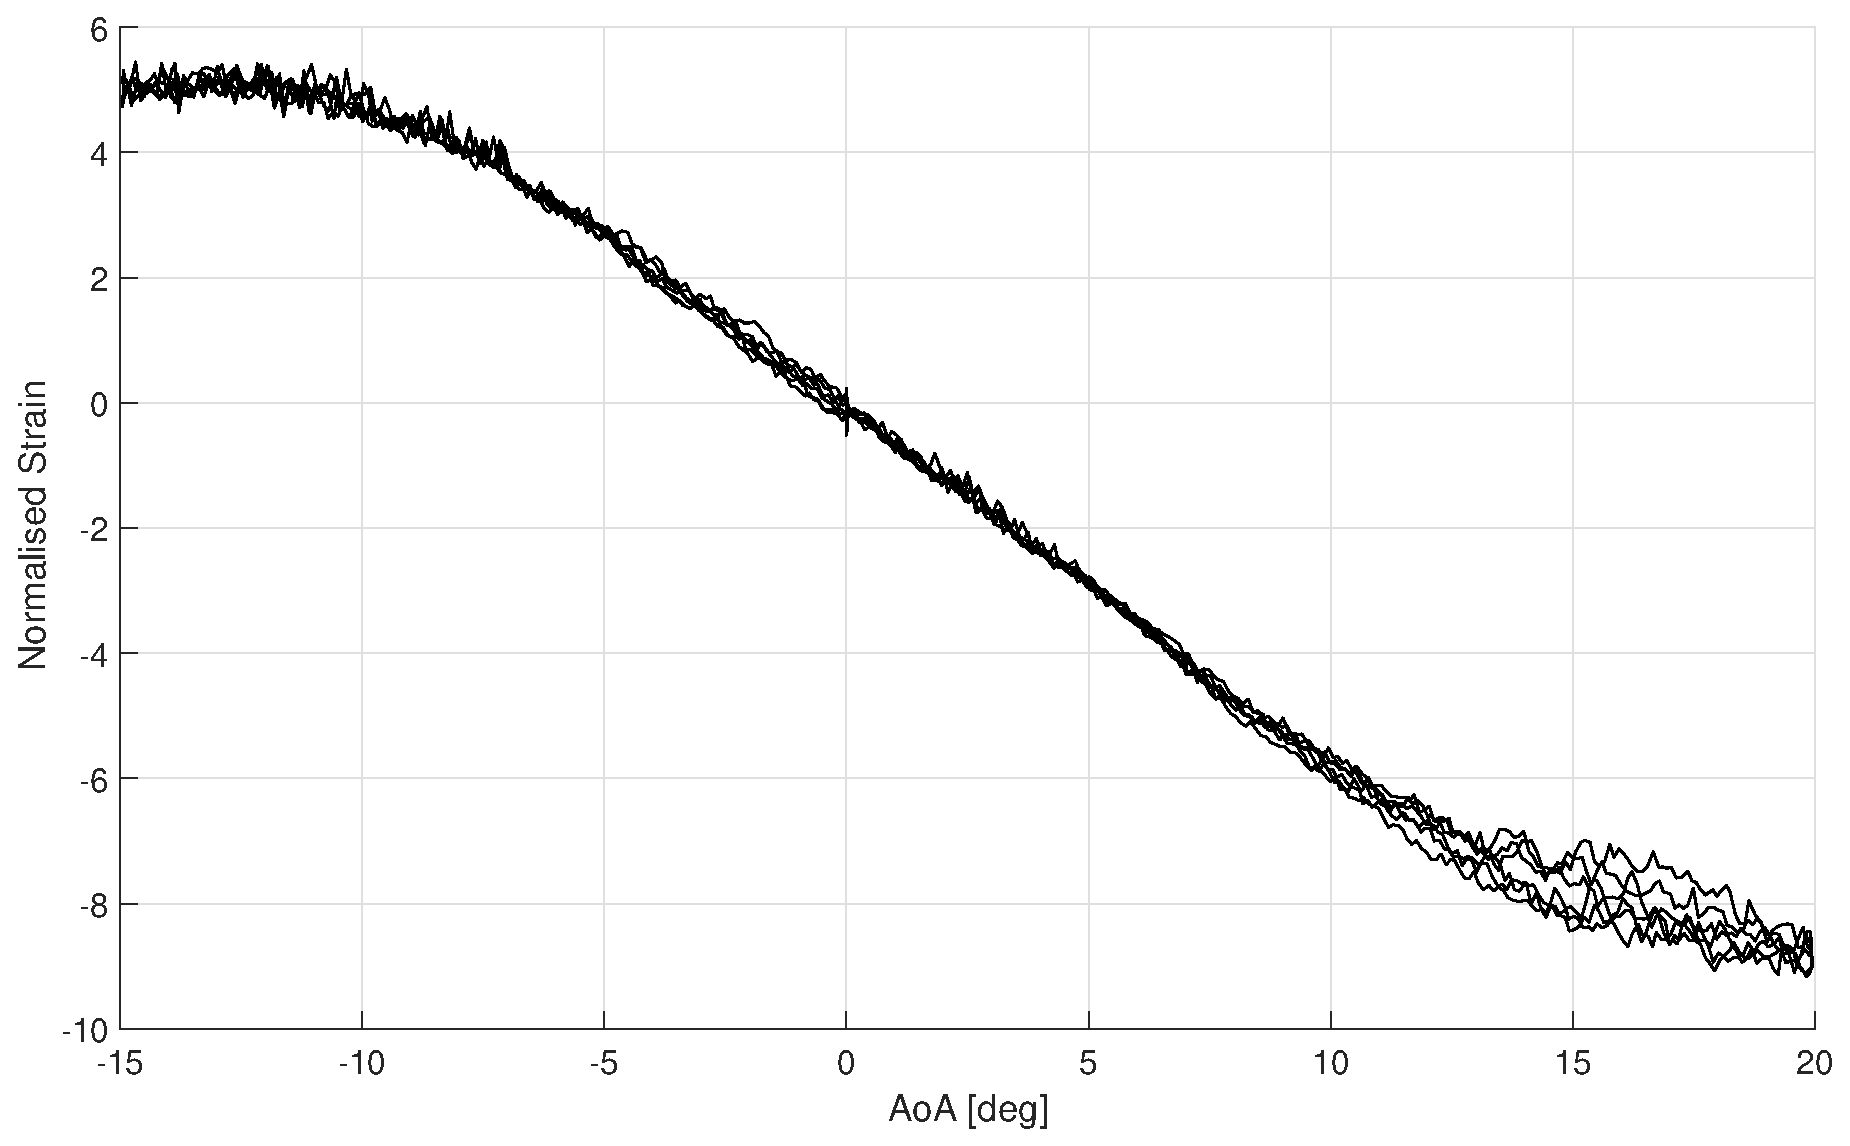
\includegraphics[width=\textwidth]{DistDataSet_P07.eps}};
		}
		\only<3>{
			\node[anchor=south west,inner sep=0] (image) at (0,0)%
				{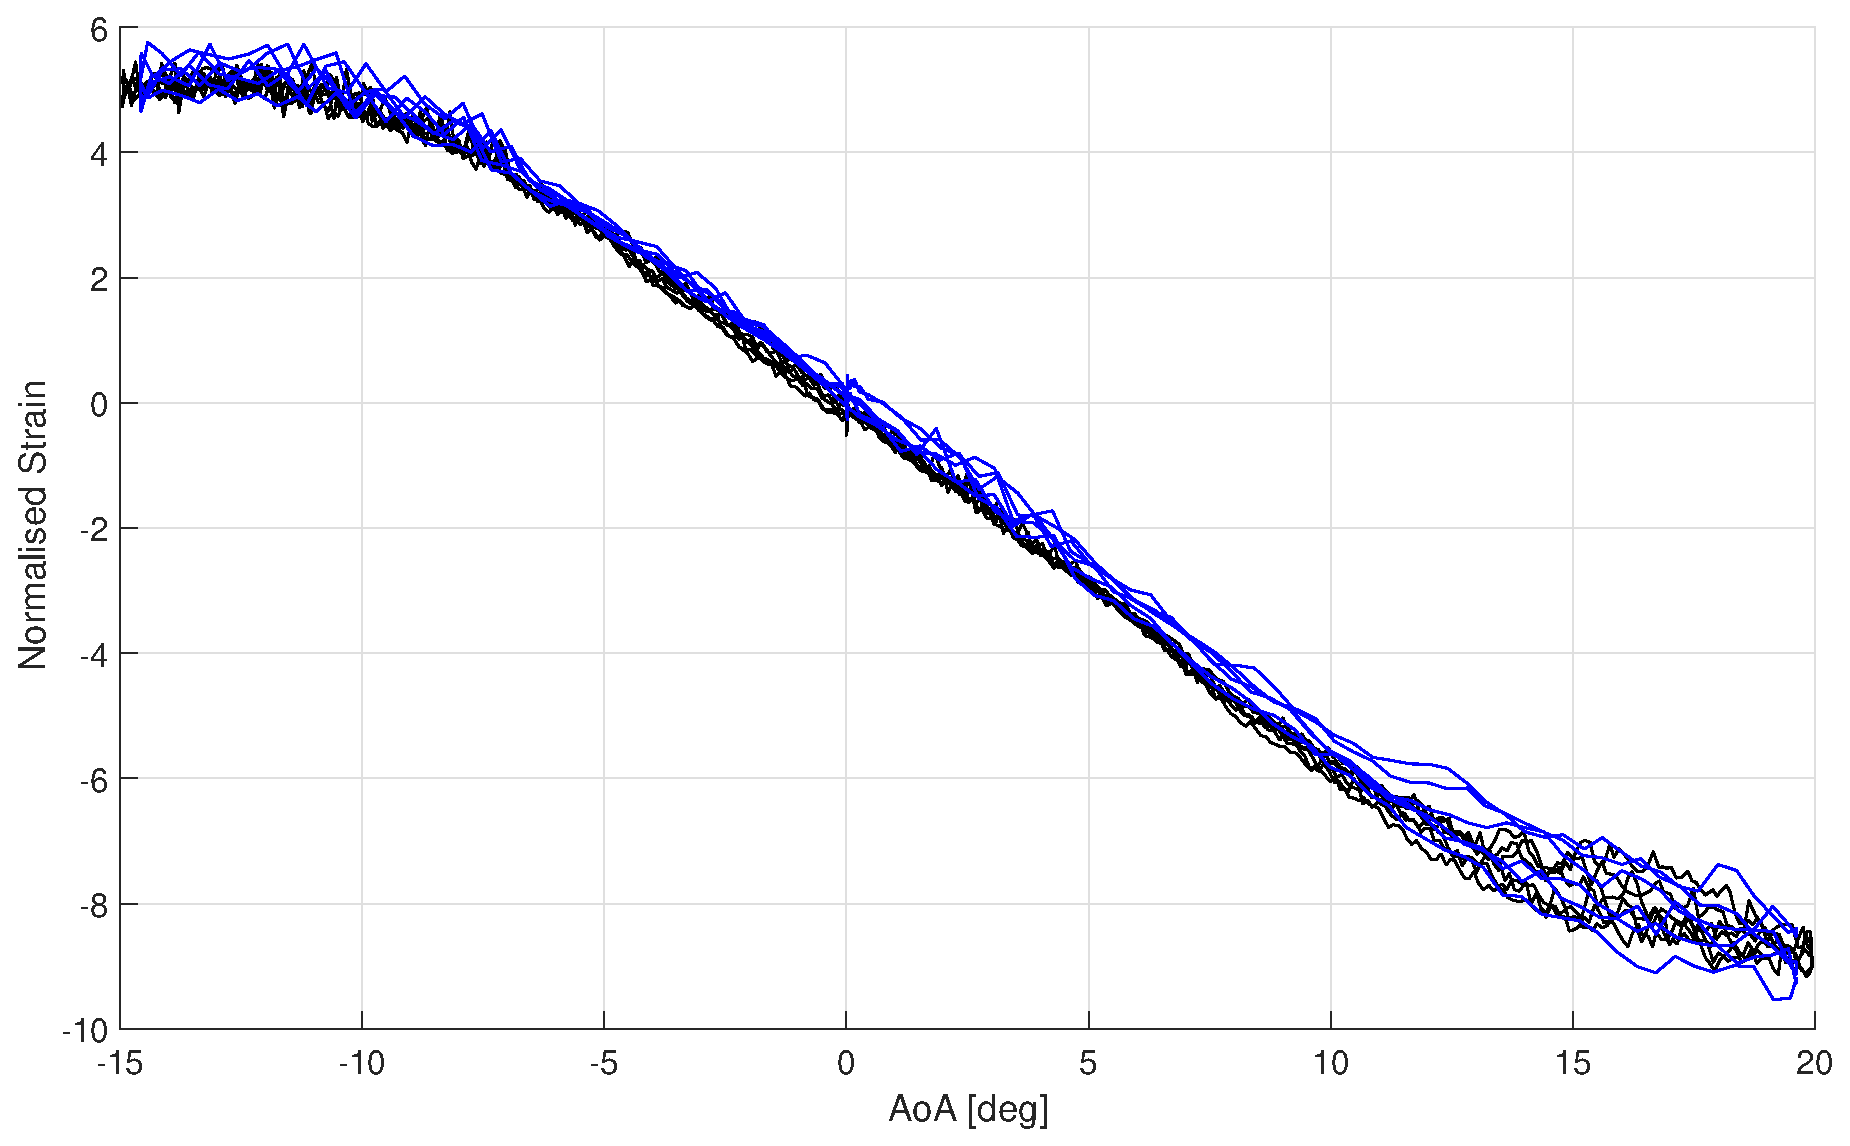
\includegraphics[width=\textwidth]{DistDataSet_P08.eps}};
		}
		\only<4->{
			\node[anchor=south west,inner sep=0] (image) at (0,0)%
				{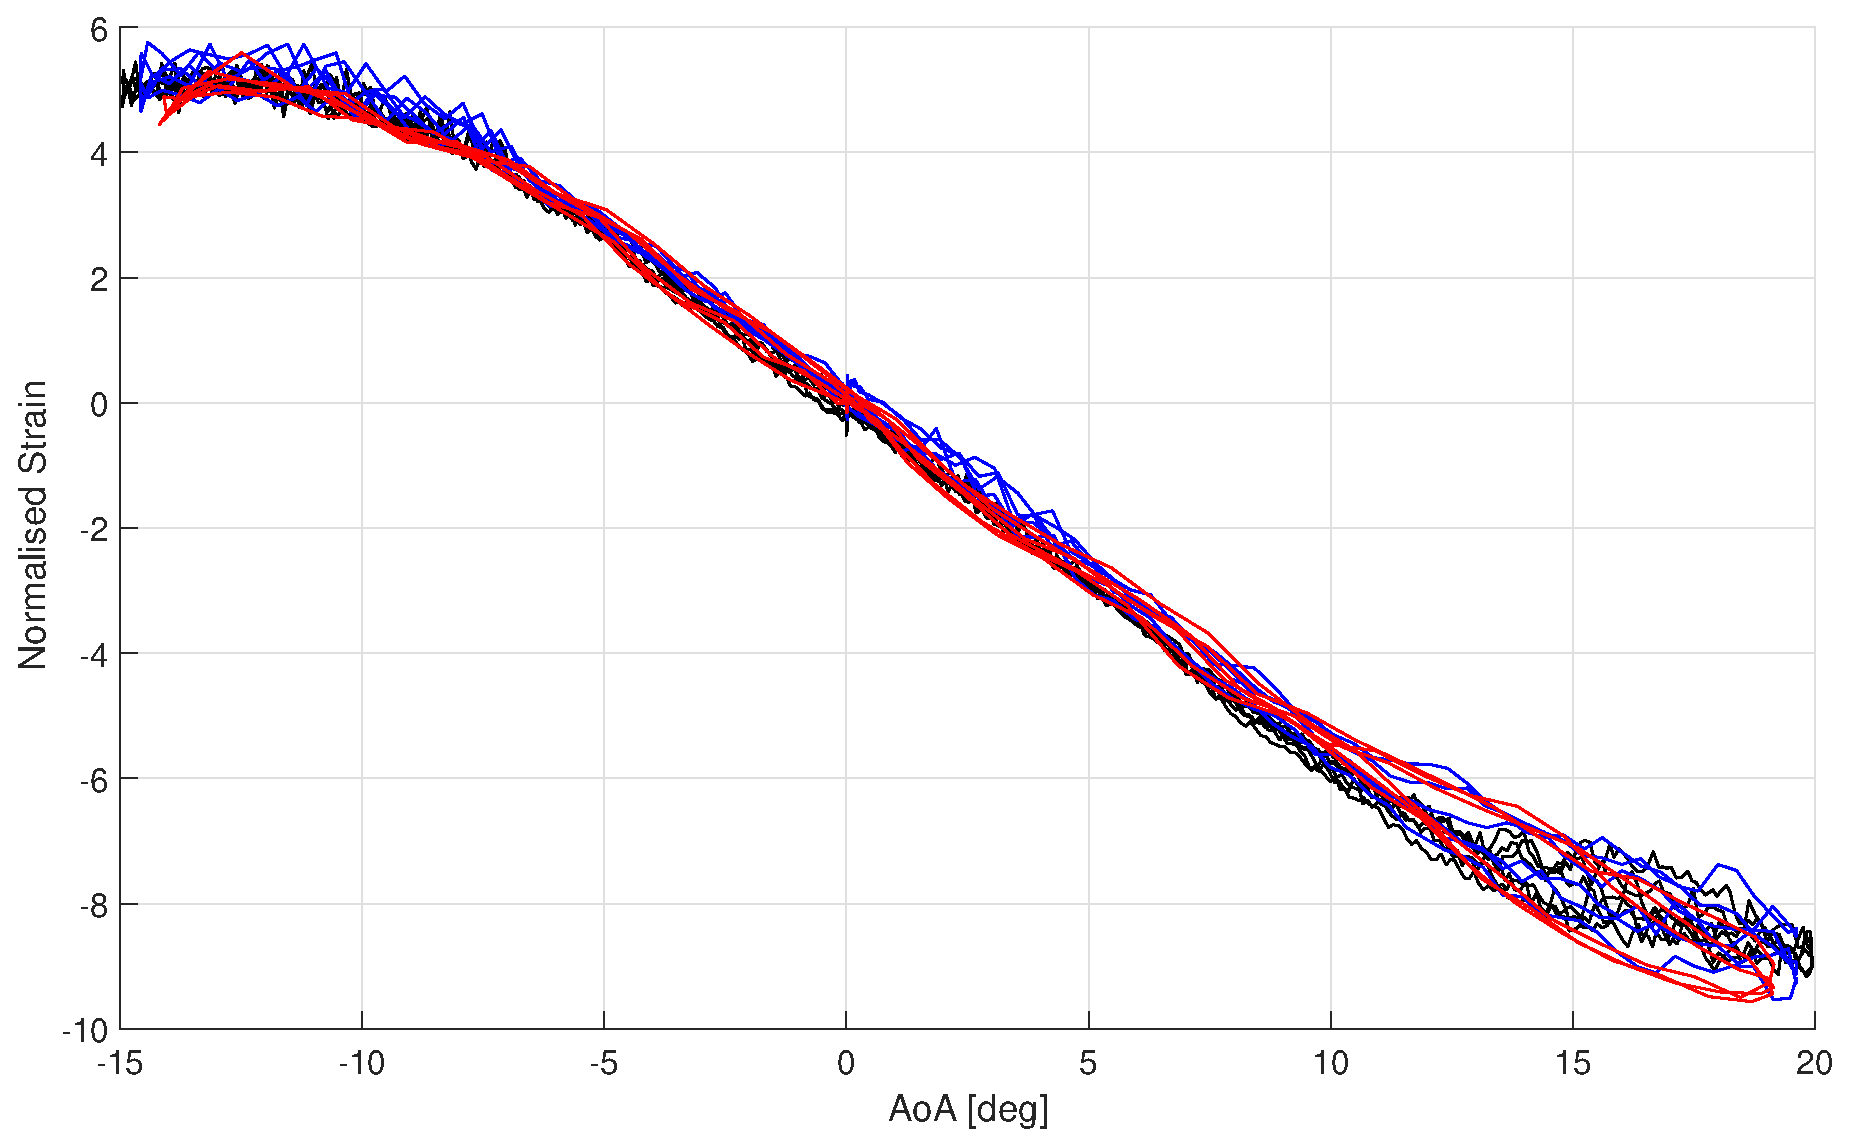
\includegraphics[width=\textwidth]{DistDataSet_P09.eps}};
		}
		%\only<5>{
			%\node[anchor=south west,inner sep=0] (image) at (0,0)%
				%{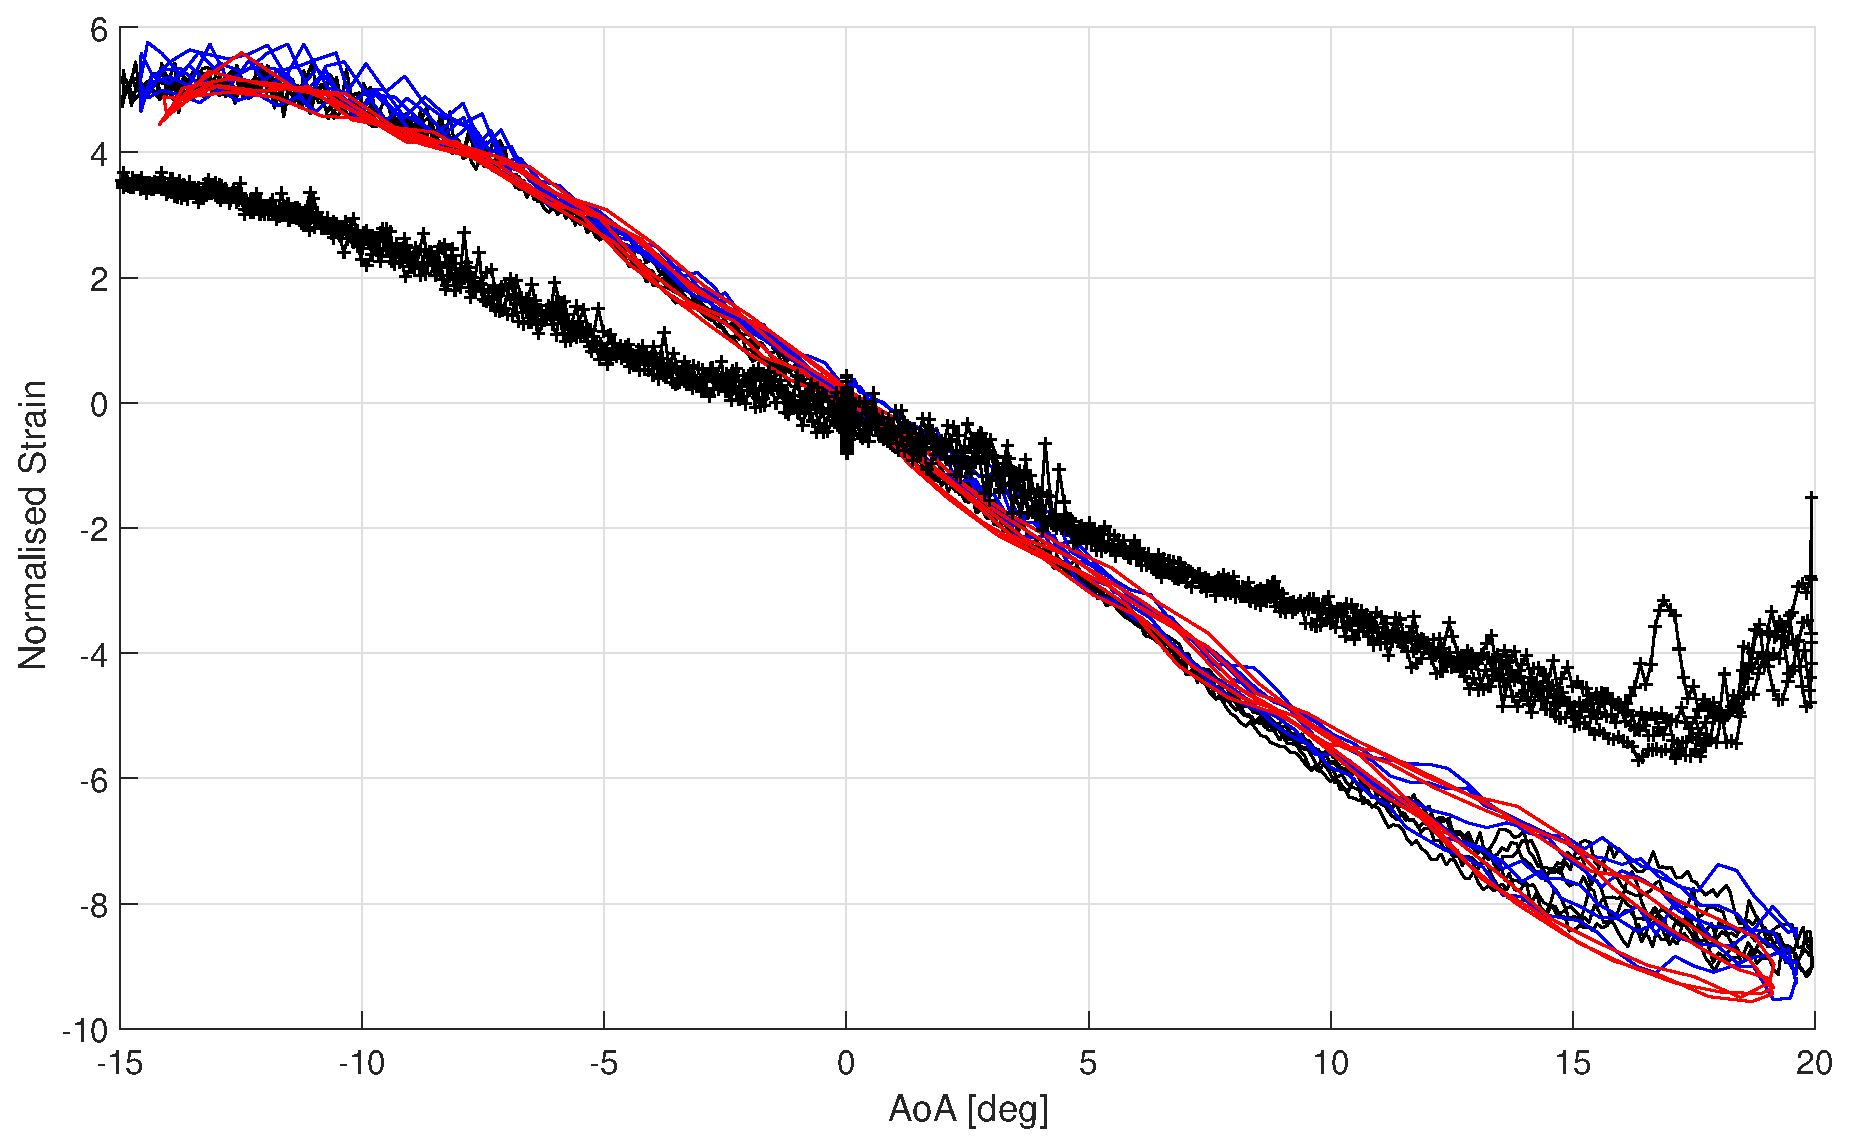
\includegraphics[width=\textwidth]{DistDataSet_P10.eps}};
		%}
		%\only<6>{
			%\node[anchor=south west,inner sep=0] (image) at (0,0)%
				%{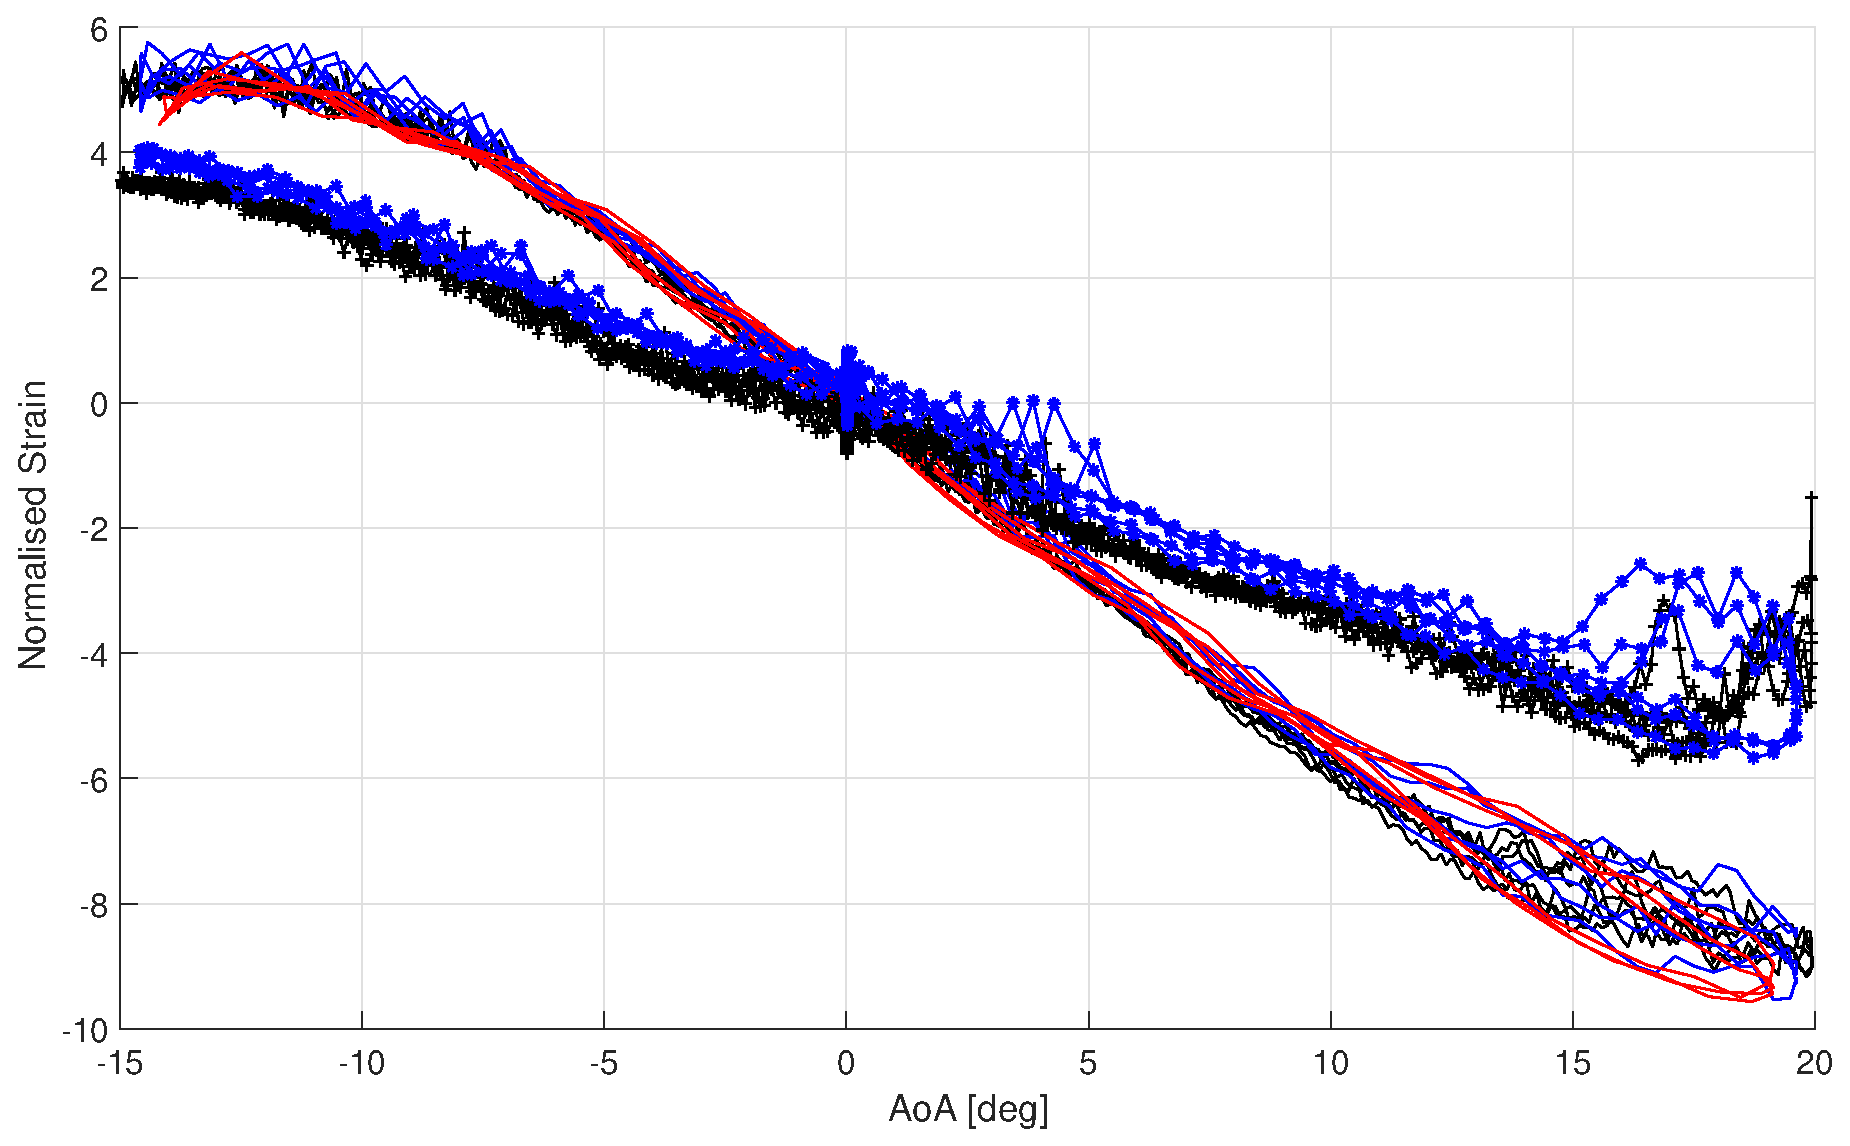
\includegraphics[width=\textwidth]{DistDataSet_P11.eps}};
		%}
		%\only<7>{
			%\node[anchor=south west,inner sep=0] (image) at (0,0)%
				%{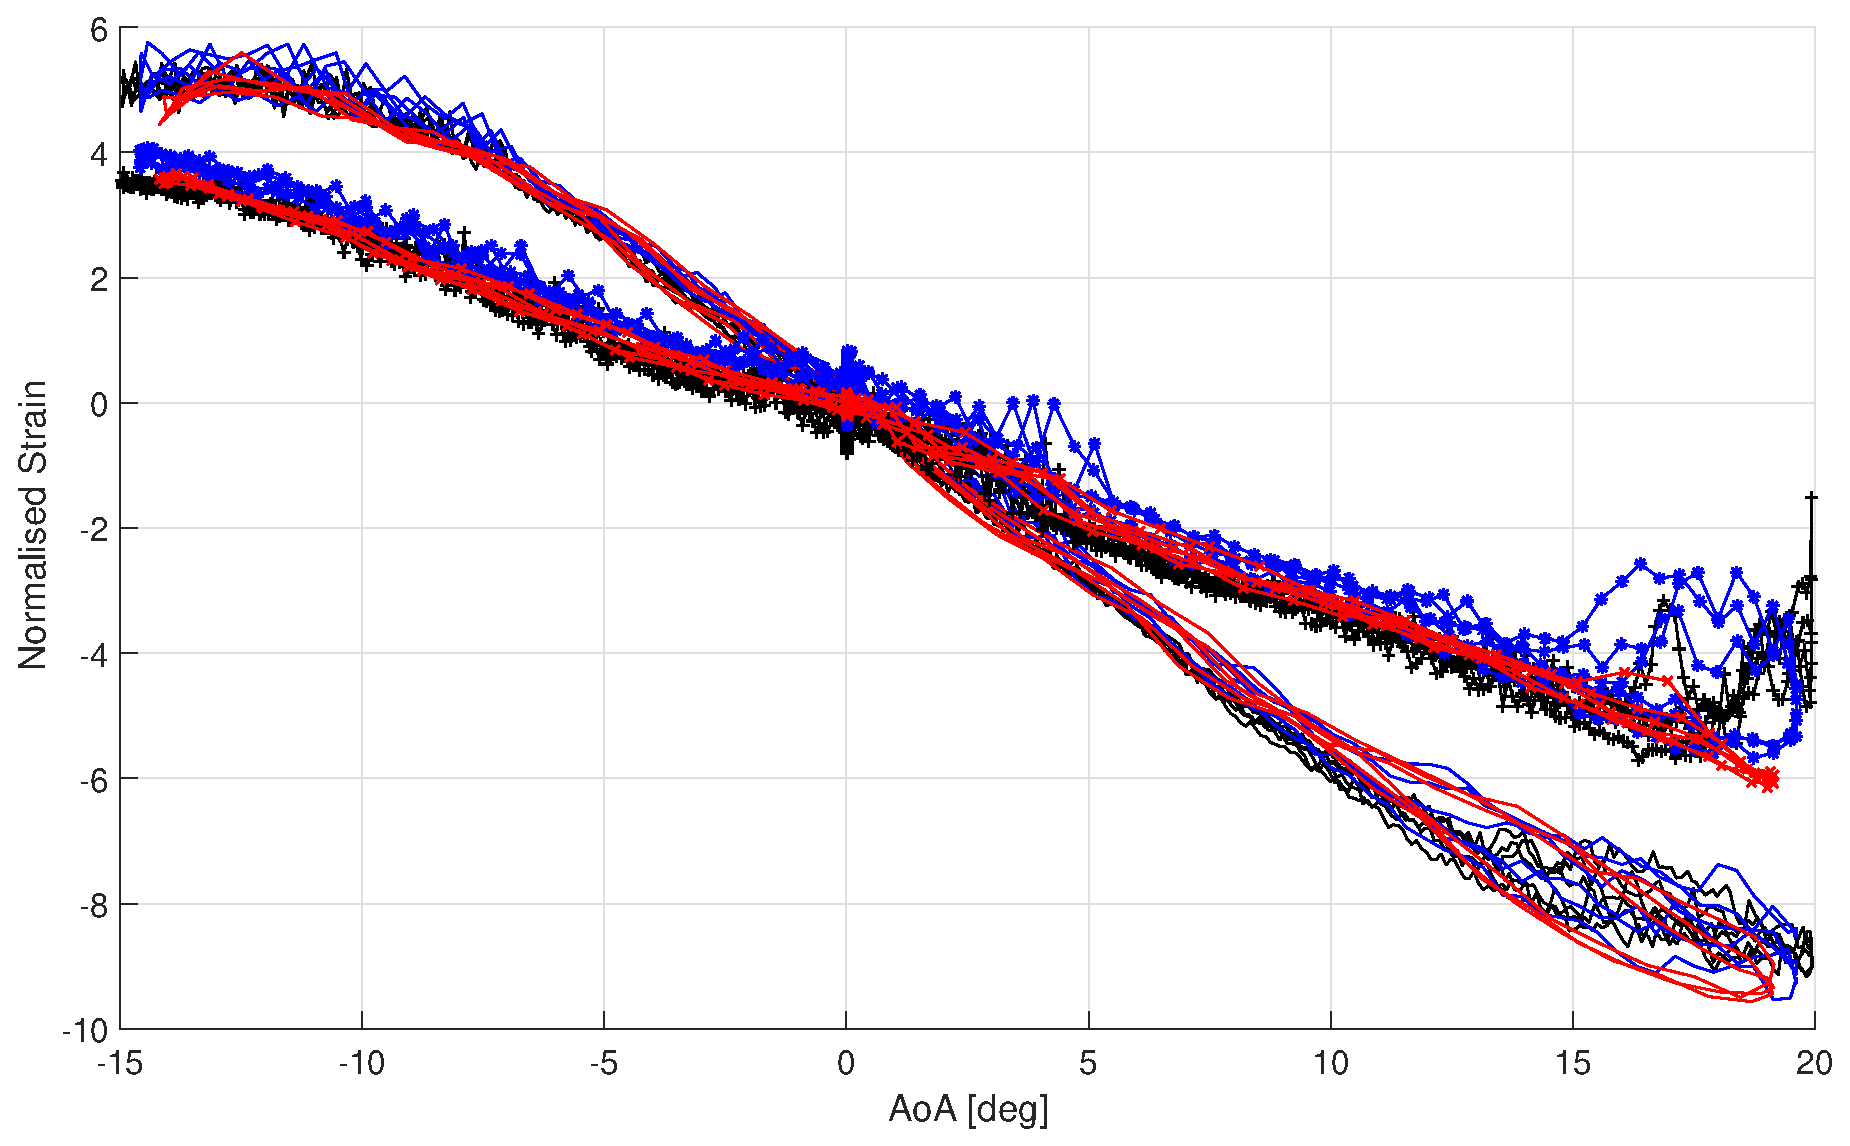
\includegraphics[width=\textwidth]{DistDataSet_P12.eps}};
		%}
		% Define scope with 'image' dimensions as reference
		\begin{scope}[x={(image.south east)},y={(image.north west)}]
			%\draw[help lines,xstep=.05,ystep=.05] (0,0) grid (1,1);
			%\foreach \x in {0,1,...,9} { \node [anchor=north] at (\x/10,0) {0.\x}; }
			%\foreach \y in {0,1,...,9} { \node [anchor=east] at (0,\y/10) {0.\y}; }
			
			% Wing node
			\draw(0.8,0.905) node (WingNode) {};
			% Wing instance
			\node[WingPlanform] (WingPlanform) at (WingNode) {};
			\draw (WingNode) ++(-0.165,0) node[WingRoot] (WingRoot) {};
			\draw (WingNode) ++(-0.075,0) node[SecObject] (SecB) {};
			\draw (WingNode) ++(+0.075,0) node[SecObject] (SecA) {};
			\draw (WingNode) ++(-0.115,0) node[SGObject] (SG_A) {};
			\draw (WingNode) ++(-0.045,0) node[SGObject] (SG_B) {};
			\draw (WingNode) ++(+0.045,0) node[SGObject] (SG_C) {};
			\draw (WingNode) ++(+0.115,0) node[SGObject] (SG_D) {};
			\only<1,2,3->{
			  %
				\draw (WingNode) ++(-0.115,0) node[SelSGObject] (SG_A) {};
			}
			%\only<4->{
			  %%
				%\draw (WingNode) ++(+0.045,0) node[SelSGObject] (SG_C) {};
			%}
			% Legend Nodes
			\draw(0.20,0.30) node (q0_Line) {};
			\draw(0.20,0.25) node (q1_Line) {};
			\draw(0.20,0.20) node (q2_Line) {};
			% Legend Arrows & Labels
			\only<1->{
			  \draw[black,line width=0.5mm] (q0_Line) -- +(-0.1,0);
				\draw(q0_Line) ++(+0.080,0) node (q0_Label) {$q = \SI[per-mode=symbol]{\pm 0.5}{\degree\per\second}$};
			}
			\only<3->{
			  \draw[blue, line width=0.5mm] (q1_Line) -- +(-0.1,0);
				\draw(q1_Line) ++(+0.075,0) node (q1_Label) {$q = \SI[per-mode=symbol]{\pm 20}{\degree\per\second}$};
			}
			\only<4->{
			  \draw[red,  line width=0.5mm] (q2_Line) -- +(-0.1,0);
				\draw(q2_Line) ++(+0.075,0) node (q2_Label) {$q = \SI[per-mode=symbol]{\pm 50}{\degree\per\second}$};
			}
			
			\only<2>{
			  % Linear Strain node
			  \draw(0.475,0.625) node (StrainAoA) {};
			  % Linear Strain marker
			  \node[Ellipseobject,rotate around={-35:(0,0)}] (StrainLinAoA) at (StrainAoA) {};
				% Linear Strain label
			  \draw(0.9,0.7) node[LabelObject] (StrainLinAoA_Label) {Strain Linear\\Response\\with AoA};
			  % Linear Strain arrow
			  \draw[ArrowObject] (StrainLinAoA_Label.west) -- (StrainLinAoA.north);
			}
			\only<5>{
			  % Linear Strain node
			  \draw(0.85,0.2) node (DynamicLift_Node) {};
			  % Linear Strain marker
			  \node[EllipseStallObject,rotate around={-25:(0,0)}] (DynamicLift) at (DynamicLift_Node) {};
				% Linear Strain label
			  \draw(0.85,0.7) node[LabelObject] (DynamicLift_Label) {Dynamic Lift};
			  % Linear Strain arrow
			  \draw[ArrowObject] (DynamicLift_Label.south) -- (DynamicLift.north);
			}
		\end{scope}
	\end{tikzpicture}
}
		\caption{Strain response for various ${q}$ values}
		\label{fig:StrainResponse2q}
  \end{figure}

\end{frame}

%%%%%%%%%%%%%%%%%%%%%%%%%%%%%%%%%%%%%%%%%%%%%%%%%%%%%%%%%%%%
%\begin{frame}{Current Research at UoB}
%
  %\begin{figure}[!htb]
    %\centering
		%% PressureResponse2q.tex

\resizebox{!}{0.3\textwidth}{
	\begin{tikzpicture}
		\only<1>{
			\node[anchor=south west,inner sep=0] (image) at (0,0)%
				{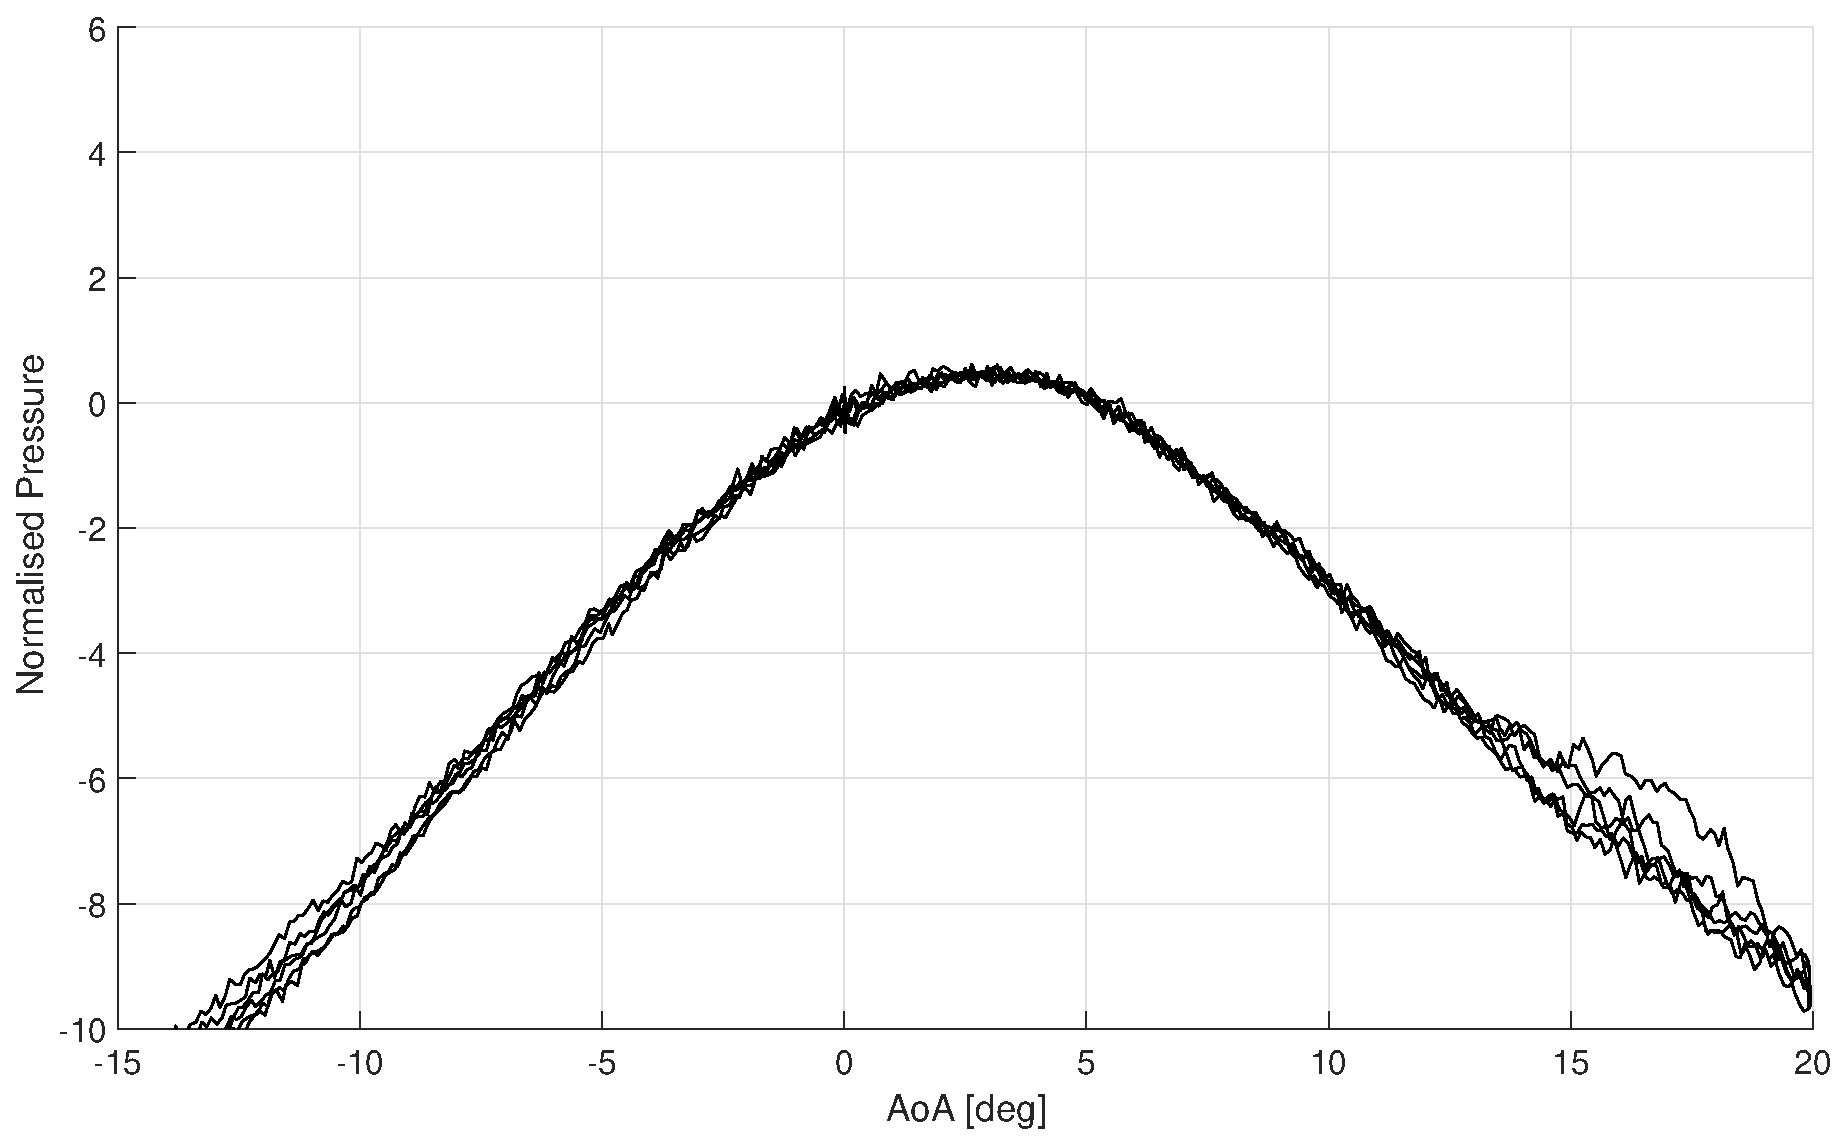
\includegraphics[width=\textwidth]{DistDataSet_P01.eps}};
		}
		\only<2>{
			\node[anchor=south west,inner sep=0] (image) at (0,0)%
				{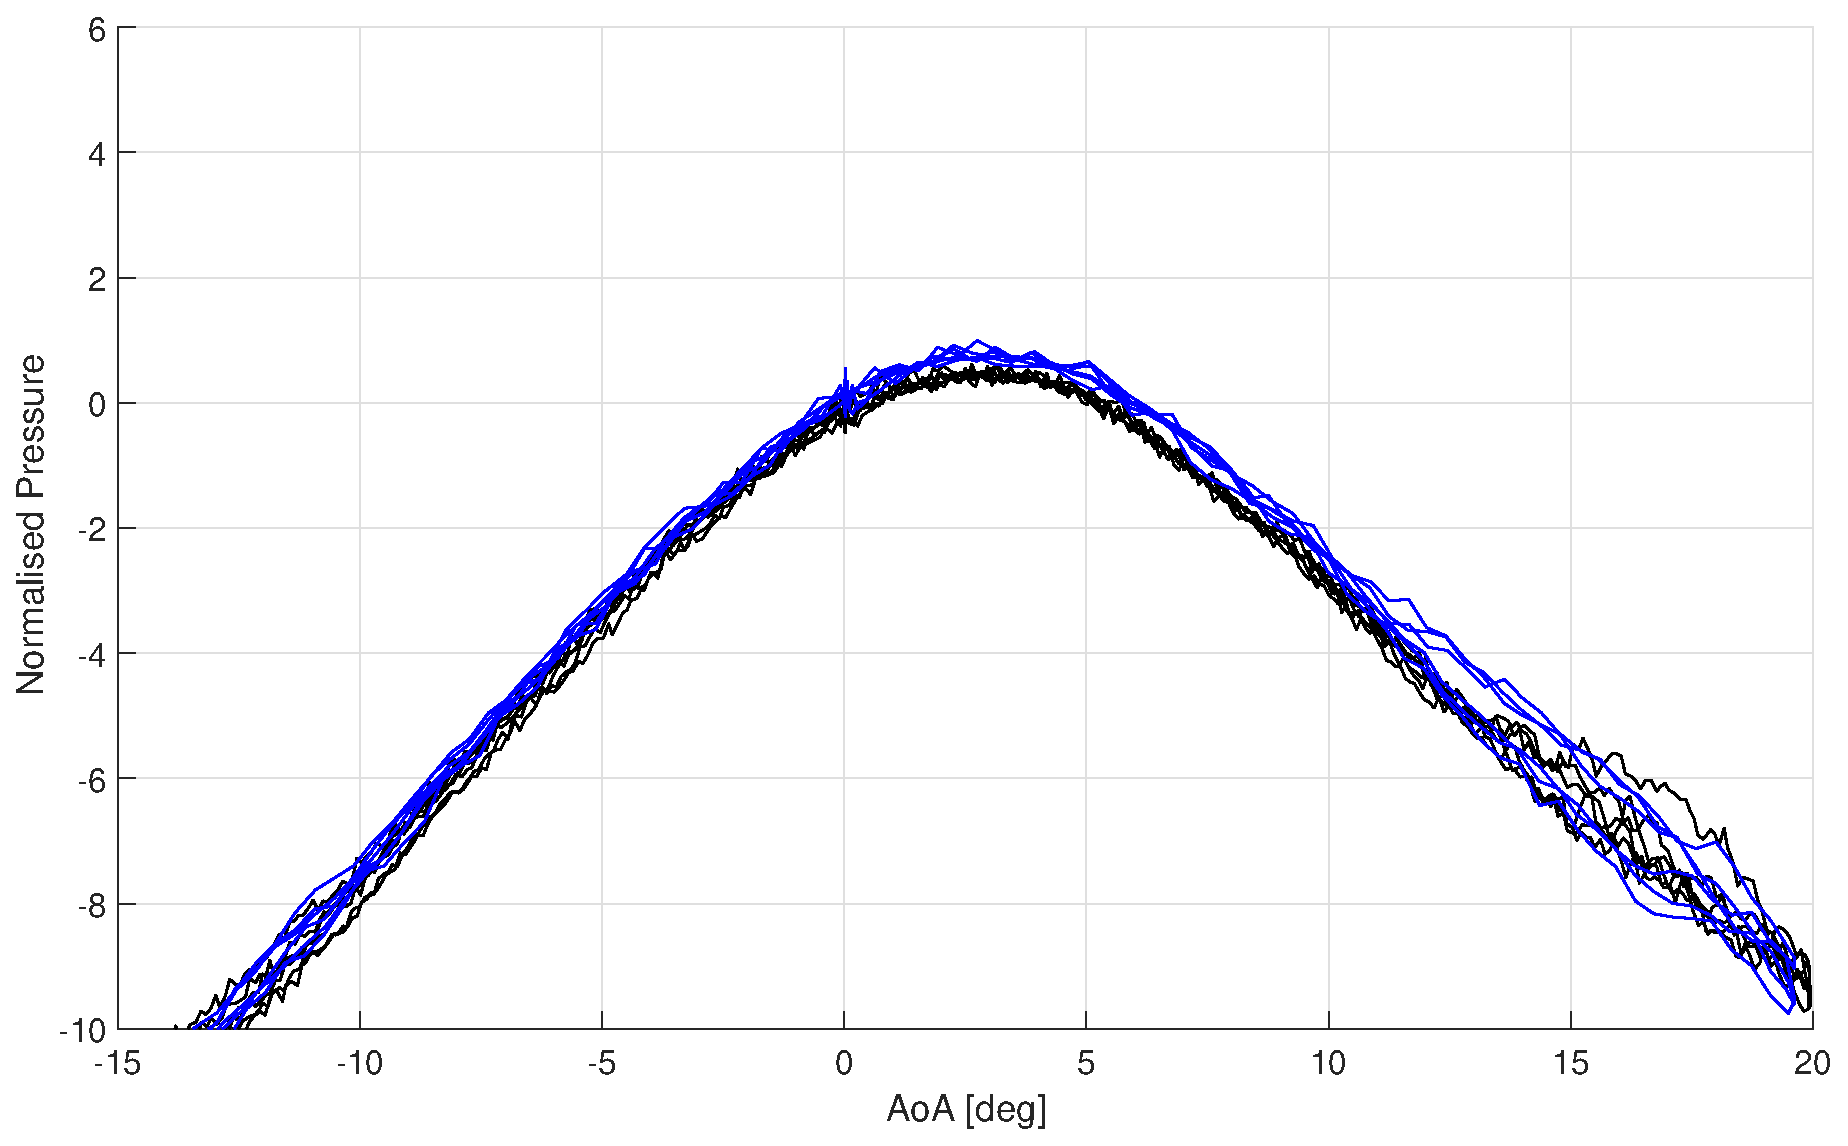
\includegraphics[width=\textwidth]{DistDataSet_P02.eps}};
		}
		\only<3>{
			\node[anchor=south west,inner sep=0] (image) at (0,0)%
				{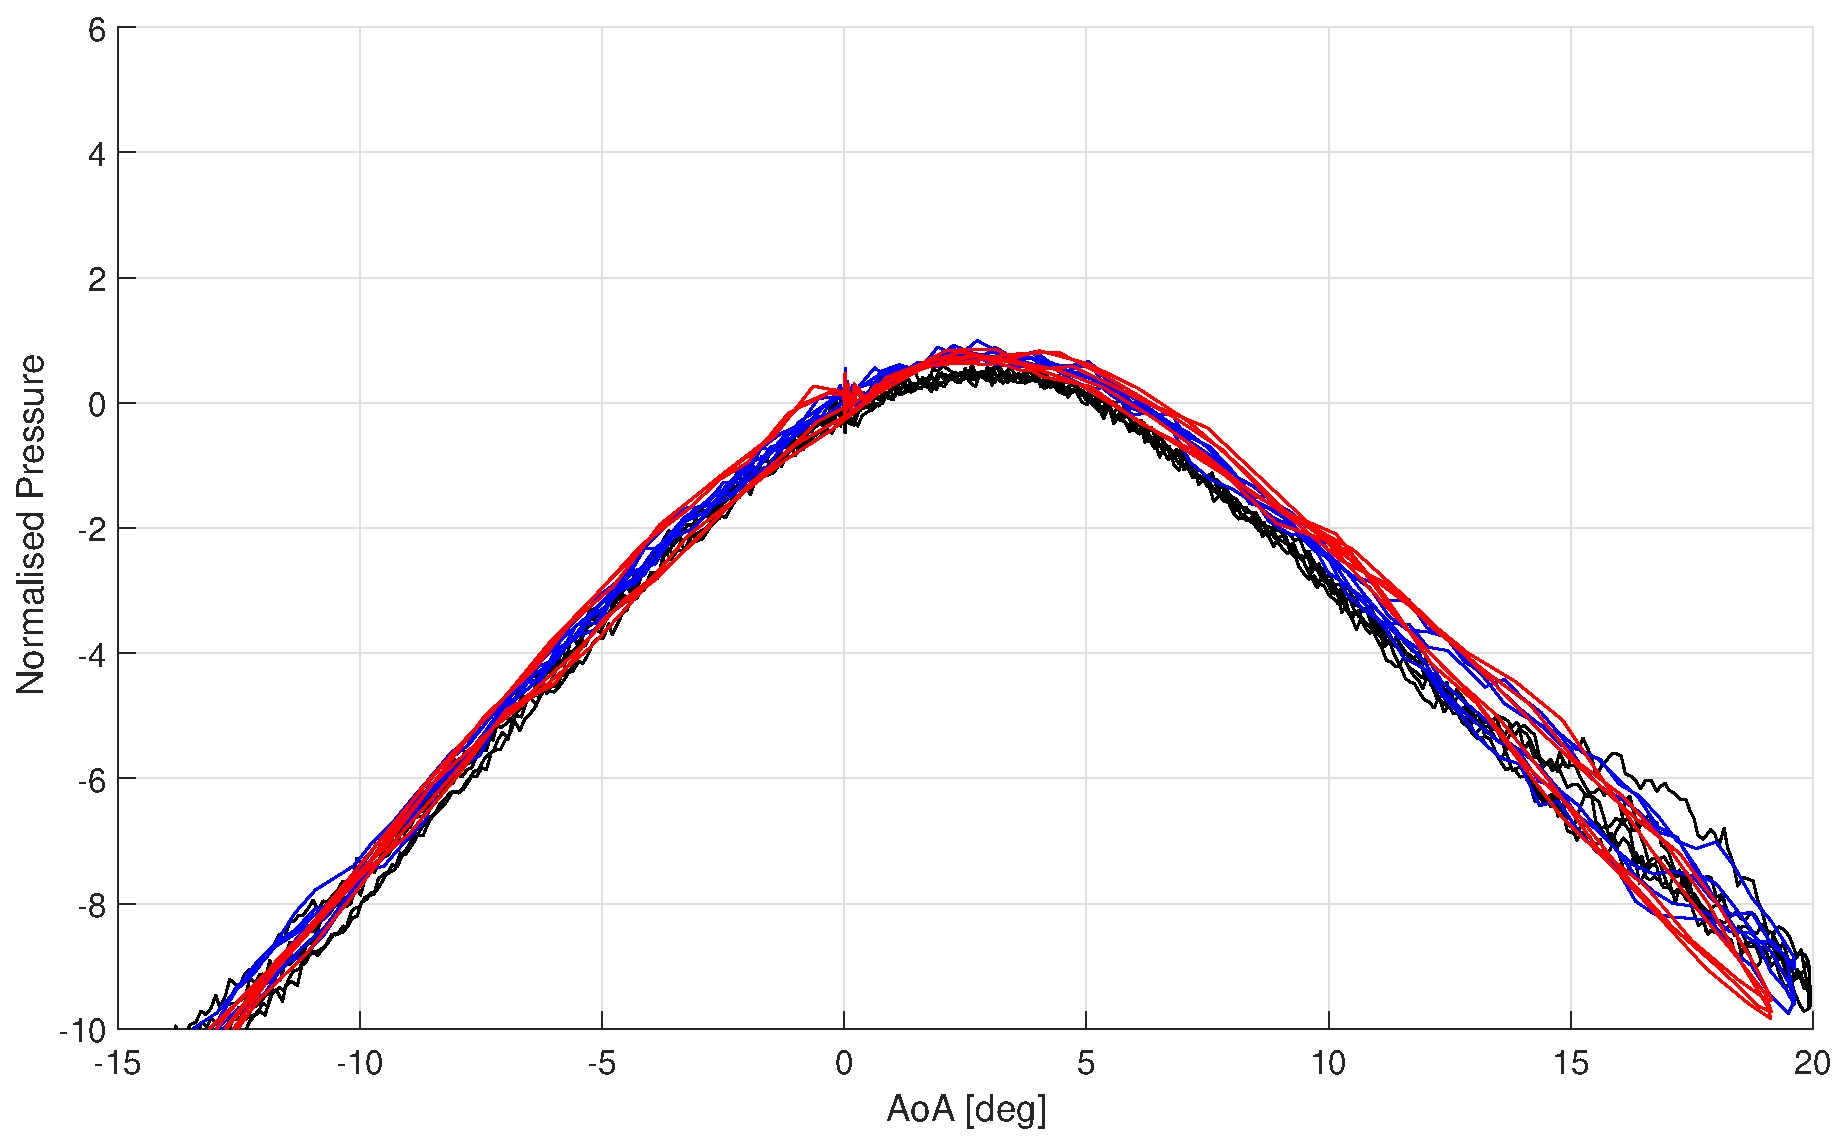
\includegraphics[width=\textwidth]{DistDataSet_P03.eps}};
		}
		\only<4>{
			\node[anchor=south west,inner sep=0] (image) at (0,0)%
				{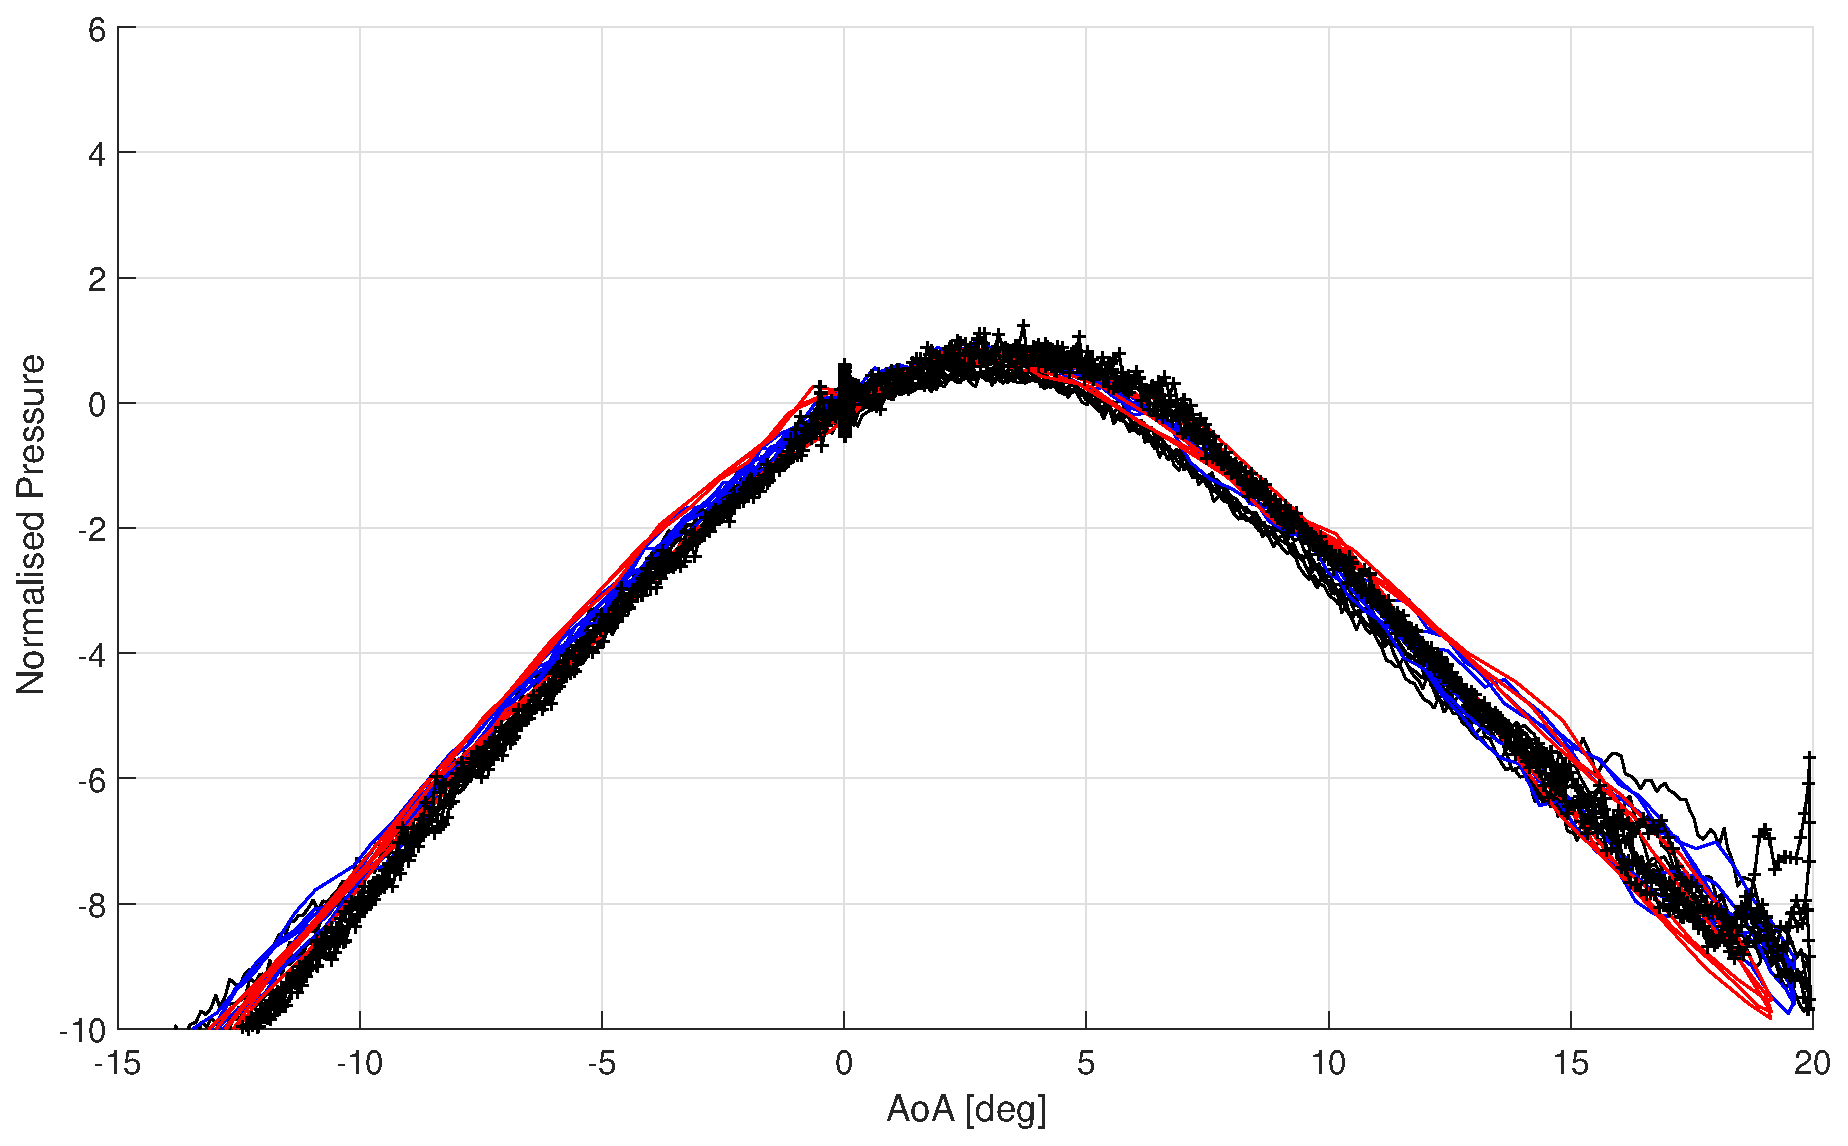
\includegraphics[width=\textwidth]{DistDataSet_P04.eps}};
		}
		\only<5>{
			\node[anchor=south west,inner sep=0] (image) at (0,0)%
				{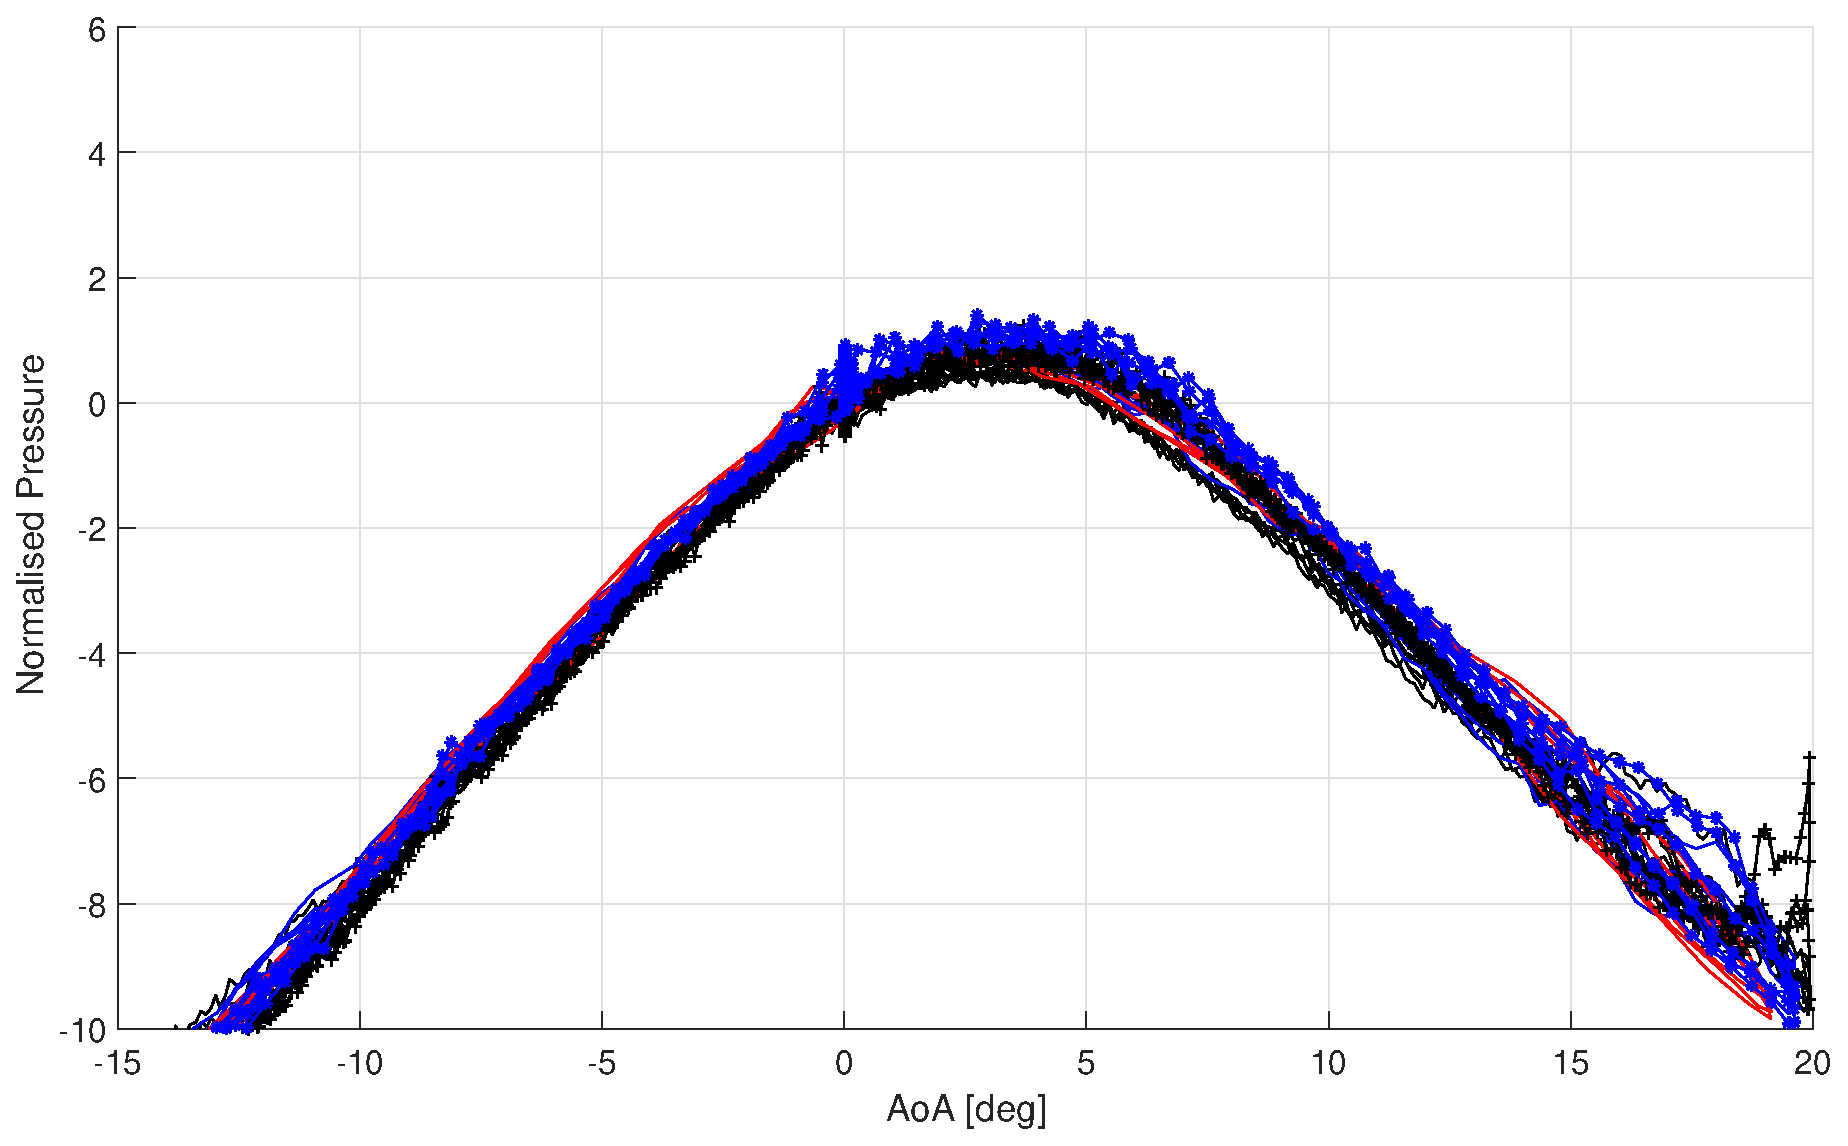
\includegraphics[width=\textwidth]{DistDataSet_P05.eps}};
		}
		\only<6>{
			\node[anchor=south west,inner sep=0] (image) at (0,0)%
				{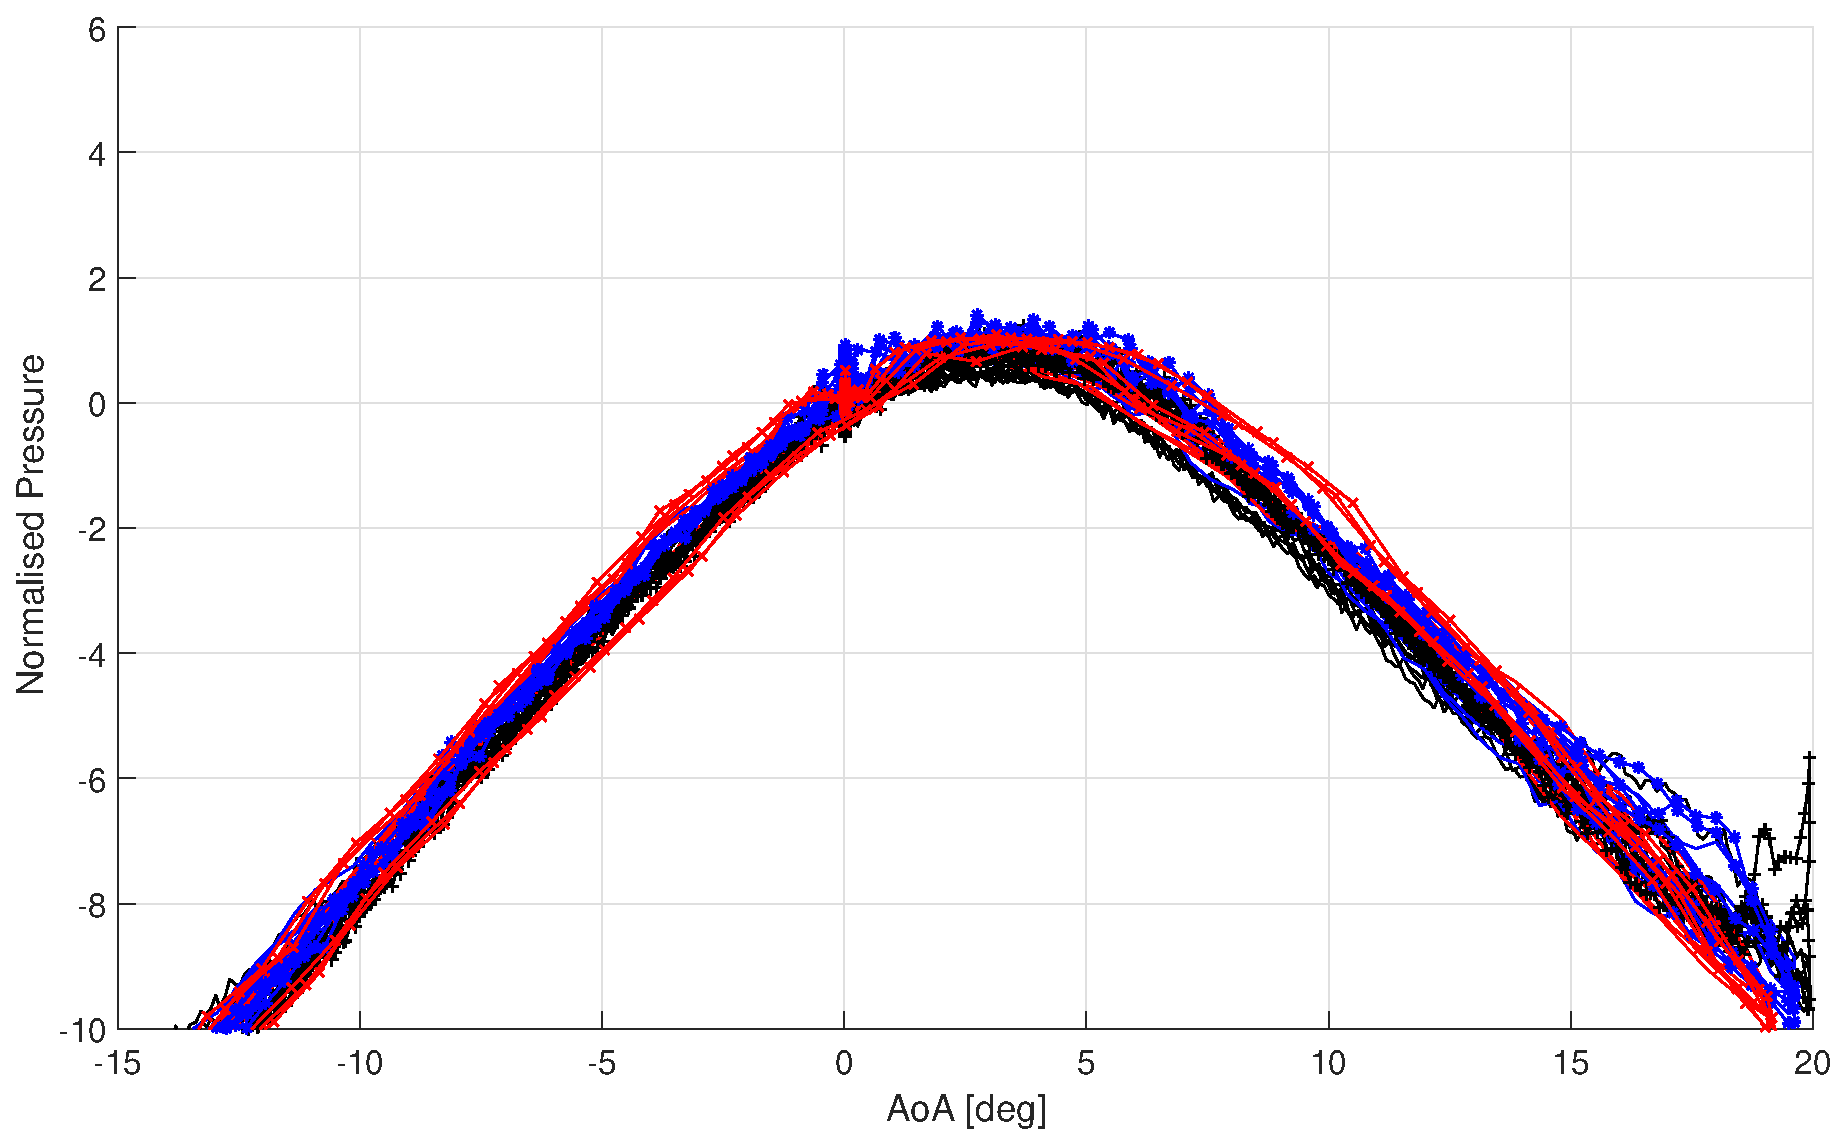
\includegraphics[width=\textwidth]{DistDataSet_P06.eps}};
		}
		% Define scope with 'image' dimensions as reference
		\begin{scope}[x={(image.south east)},y={(image.north west)}]
			%\draw[help lines,xstep=.05,ystep=.05] (0,0) grid (1,1);
			%\foreach \x in {0,1,...,9} { \node [anchor=north] at (\x/10,0) {0.\x}; }
			%\foreach \y in {0,1,...,9} { \node [anchor=east] at (0,\y/10) {0.\y}; }
			
		\end{scope}
	\end{tikzpicture}
}
		%\caption{Pressure response for various ${q}$ values}
		%\label{fig:PressureResponse2q}
  %\end{figure}
%
%\end{frame}

%%%%%%%%%%%%%%%%%%%%%%%%%%%%%%%%%%%%%%%%%%%%%%%%%%%%%%%%%%%%
\begin{frame}{Current Research at UoB}

  \begin{figure}[!htb]
    \centering
		% DistSens_DynResponse.tex

\tikzstyle{Ellipseobject}=[ultra thick, draw=blue, ellipse, minimum width=30em,
    minimum height=8em,align=center]
\tikzstyle{LabelObject}=[draw=black, fill=white,rectangle,rounded corners,line width=0.5mm,%
	  align=center]
\tikzstyle{ArrowObject}=[red,line width=1.0mm, -latex]
\tikzstyle{WingRoot}=[draw=black, fill=white,rectangle,line width=0.25mm,%
	  align=center,minimum width=0.25em,minimum height=4.5em,pattern=north west lines]
\tikzstyle{WingPlanform}=[draw=black, fill=white,rectangle,line width=0.25mm,%
	  align=center,minimum width=14.24em,minimum height=3em]
\tikzstyle{SecObject}=[draw=black, rectangle,line width=0.25mm,%
	  align=center,minimum width=1em,minimum height=3em]
\tikzstyle{SelSecObject}=[draw=black, fill=blue,rectangle,line width=0.25mm,%
	  align=center,minimum width=1em,minimum height=3em]
\tikzstyle{SGObject}=[draw=black, rectangle,line width=0.25mm,%
	  align=center,minimum width=1em,minimum height=1em]
\tikzstyle{SelSGObject}=[draw=black, fill=blue,rectangle,line width=0.25mm,%
	  align=center,minimum width=1em,minimum height=1em]

\resizebox{!}{0.3\textwidth}{
	\begin{tikzpicture}
	  \node[anchor=south west,inner sep=0] (image) at (0,0)%
				{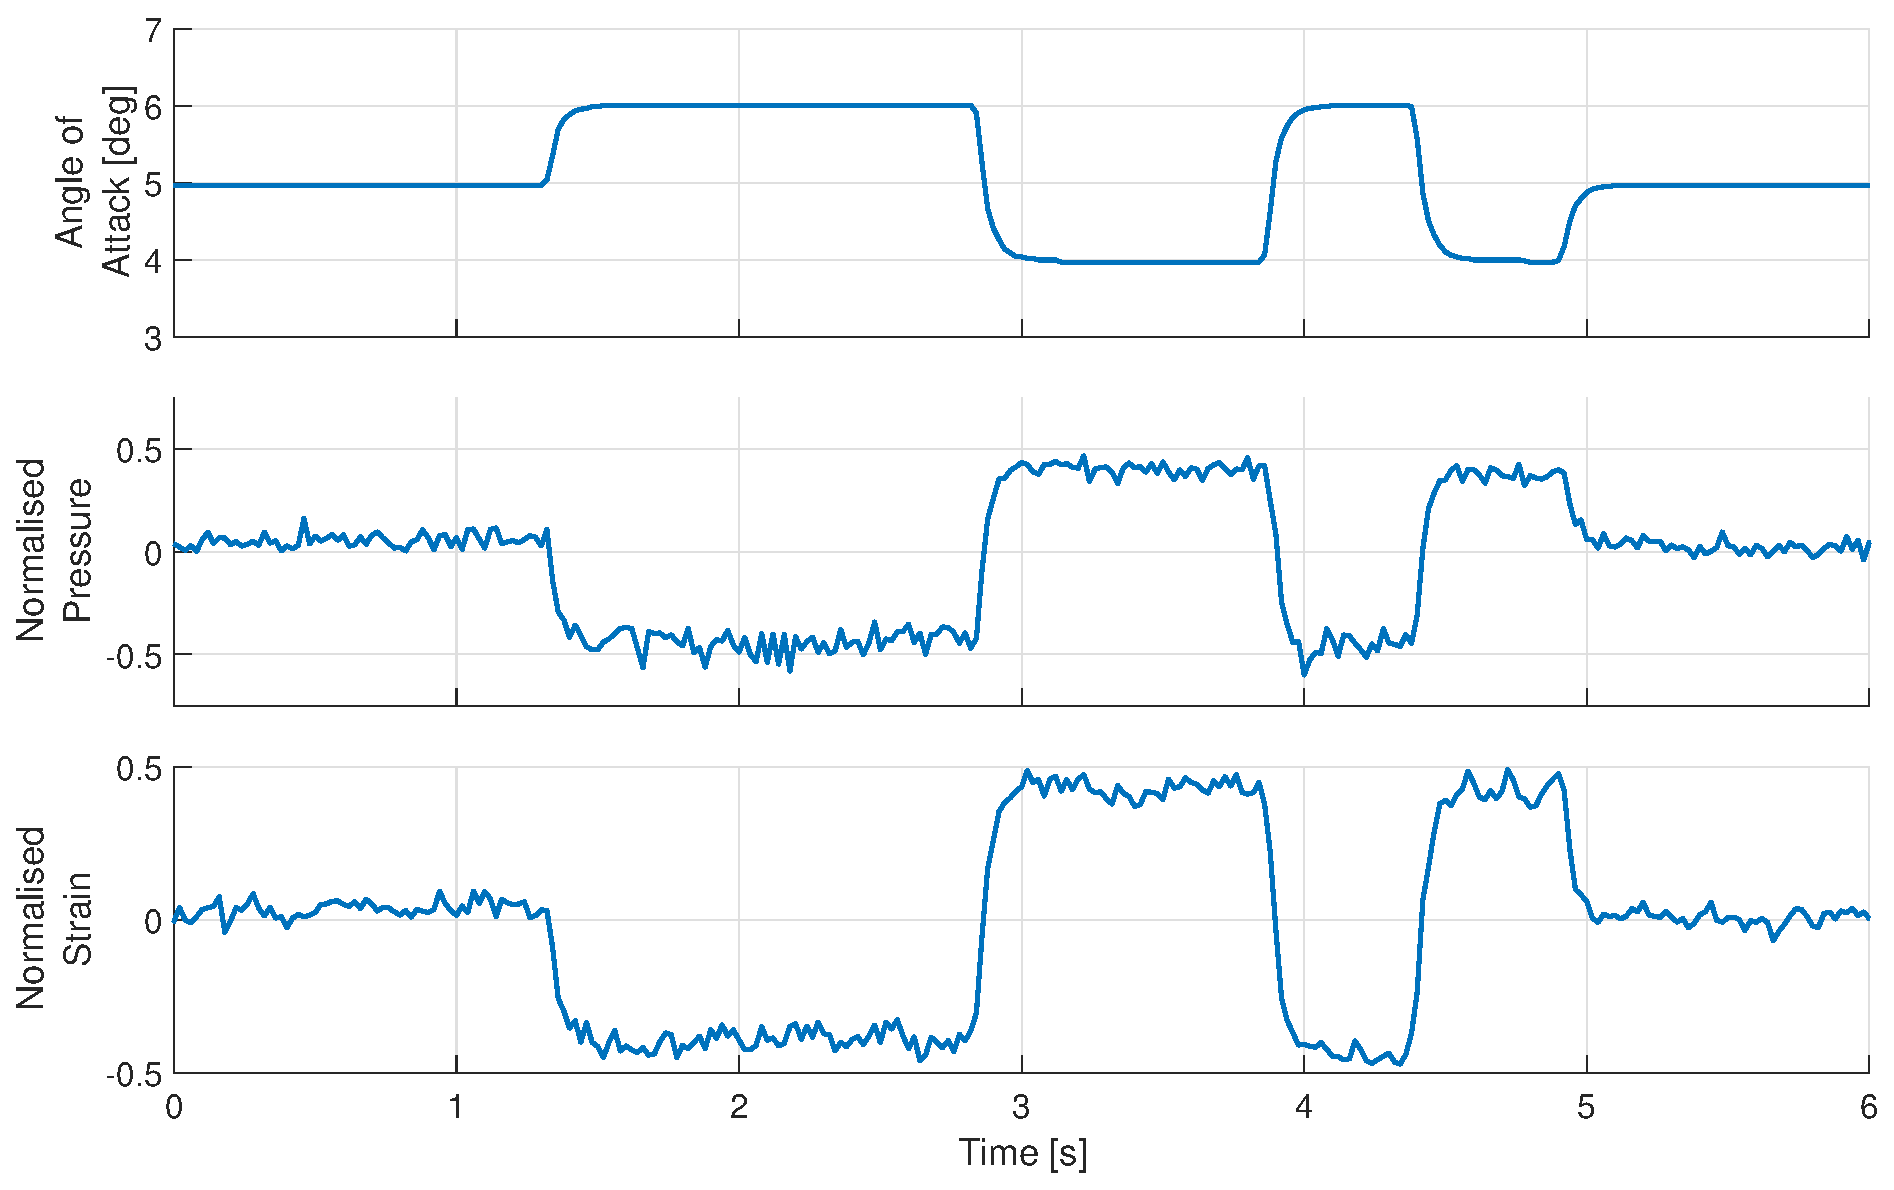
\includegraphics[width=\textwidth]{DistDataSet_P13.eps}};
		% Define scope with 'image' dimensions as reference
		\begin{scope}[x={(image.south east)},y={(image.north west)}]
			%\draw[help lines,xstep=.05,ystep=.05] (0,0) grid (1,1);
			%\foreach \x in {0,1,...,9} { \node [anchor=north] at (\x/10,0) {0.\x}; }
			%\foreach \y in {0,1,...,9} { \node [anchor=east] at (0,\y/10) {0.\y}; }
			
			\only<2>{
			  % Input node
			  \draw(0.575,0.85) node (ServoInput) {};
			  % Input marker
			  \node[Ellipseobject] (ServoInputTimeHist) at (ServoInput) {};
			  % Input label
			  \draw(0.4,0.4) node[LabelObject] (ServoInput_Label) {Rig Servo\\3-2-1-1 Input};
			  % Input arrows
			  \draw[ArrowObject] (ServoInput_Label.north east) -- (ServoInputTimeHist.south);
			}
			\only<3>{
			  % Input node
			  \draw(0.575,0.525) node (PressureResponse) {};
			  % Input marker
			  \node[Ellipseobject] (PressureResponseTimeHist) at (PressureResponse) {};
			  % Input label
			  \draw(0.4,0.15) node[LabelObject] (PressureResponse_Label) {Pressure Response\\Section A ${0.4 c}$ Sensor};
			  % Input arrows
			  \draw[ArrowObject] (PressureResponse_Label.north east) -- (PressureResponseTimeHist.south);
				
				% Airfoil node
			  \draw(0.1,0.85) node (AirfoilNode) {};
				% Airfoil
				\node (Airfoil) at (AirfoilNode) {%
				  \begin{axis}[
					  unit vector ratio*=1 1 1, % keeps a 1:1 scale between x and y axis
					  width=8cm,
						height=3cm,
						xmin=-0.1,
            xmax= 1.1,
						xticklabels={,,},
						yticklabels={,,},
            tick style={draw=none},
						axis on top,
						axis background/.style={fill=white},
						]
				      \addplot[smooth] table [x=x, y=y, col sep=comma] {./Figures/WOT4Airfoil.dat};
							\addplot[smooth,mark=*,blue] plot coordinates {
                (0.4,0.09)
                };
					\end{axis}
				};
				
				% Wing node
			  \draw(0.8,0.905) node (WingNode) {};
			  % Wing instance
			  \node[WingPlanform] (WingPlanform) at (WingNode) {};
				\draw (WingNode) ++(-0.165,0) node[WingRoot] (WingRoot) {};
				\draw (WingNode) ++(-0.075,0) node[SelSecObject] (SecB) {};
				\draw (WingNode) ++(+0.075,0) node[SecObject] (SecA) {};
				\draw (WingNode) ++(-0.115,0) node[SGObject] (SG_A) {};
				\draw (WingNode) ++(-0.045,0) node[SGObject] (SG_B) {};
				\draw (WingNode) ++(+0.045,0) node[SGObject] (SG_C) {};
				\draw (WingNode) ++(+0.115,0) node[SGObject] (SG_D) {};
			}
			\only<4>{
			  % Input node
			  \draw(0.575,0.225) node (StrainResponse) {};
			  % Input marker
			  \node[Ellipseobject] (StrainResponseTimeHist) at (StrainResponse) {};
			  % Input label
			  \draw(0.4,0.6) node[LabelObject] (StrainResponse_Label) {Strain Response\\Section B Inboard Sensor};
			  % Input arrows
			  \draw[ArrowObject] (StrainResponse_Label.south east) -- (StrainResponseTimeHist.north);
				
				% Wing node
			  \draw(0.8,0.905) node (WingNode) {};
			  % Wing instance
			  \node[WingPlanform] (WingPlanform) at (WingNode) {};
				\draw (WingNode) ++(-0.165,0) node[WingRoot] (WingRoot) {};
				\draw (WingNode) ++(-0.075,0) node[SecObject] (SecB) {};
				\draw (WingNode) ++(+0.075,0) node[SecObject] (SecA) {};
				\draw (WingNode) ++(-0.115,0) node[SelSGObject] (SG_A) {};
				\draw (WingNode) ++(-0.045,0) node[SGObject] (SG_B) {};
				\draw (WingNode) ++(+0.045,0) node[SGObject] (SG_C) {};
				\draw (WingNode) ++(+0.115,0) node[SGObject] (SG_D) {};
			}
			
		\end{scope}
	\end{tikzpicture}
}
		\caption{Pressure \& strain response to dynamic input}
		\label{fig:DistSens_DynResponse}
  \end{figure}

\end{frame}

%%%%%%%%%%%%%%%%%%%%%%%%%%%%%%%%%%%%%%%%%%%%%%%%%%%%%%%%%%%%
\begin{frame}{Current Research at UoB}

  \vspace{-1.5em}
	\begin{columns}
	  \begin{column}{0.6\textwidth}
		  \begin{figure}[!htb]
        \centering
				% ANN_UAVCtrl_BlockDiagram.tex
\tikzset{%
  every neuron/.style={
    circle,
    draw,
    minimum size=1cm,
		line width=1.0mm
  },
  neuron missing/.style={
    draw=none, 
    scale=4,
    text height=0.333cm,
    execute at begin node=\color{black}$\vdots$
  },
}
\tikzstyle{ArrowObject1}=[line width=1.5mm, -latex]
\tikzstyle{ArrowObject2}=[line width=1.5mm, latex-]
\resizebox{!}{0.45\textwidth}{
	\begin{tikzpicture}[x=1.5cm, y=1.5cm, >=stealth]
		%\draw[help lines,xstep=.5,ystep=.5] (-3,-3) grid (8,4);
		%\foreach \x in {-3,-2,...,8} { \node [anchor=north] at (\x/1,0) {0.\x}; }
		%\foreach \y in {-3,-2,...,4} { \node [anchor=east] at (0,\y/1) {0.\y}; }
		
		% Input layer nodes
		\foreach \m/\l [count=\y] in {1,2,3}
			\node [every neuron/.try, neuron \m/.try] (input-\m) at (0,2.5-\y) {};
		% Hidden layer nodes
		\foreach \m [count=\y] in {1,2,3,missing,4}
			\node [every neuron/.try, neuron \m/.try ] (hidden-\m) at (3,4.0-\y*1.10) {};
		% Output layer nodes
		\foreach \m [count=\y] in {1,2,missing,3}
			\node [every neuron/.try, neuron \m/.try ] (output-\m) at (6,3.0-\y) {};

		% Input layer labels
		%\foreach \l [count=\i] in {1,2,3}
			\draw [ArrowObject2] (input-1) -- ++(-2.0,0)
				node [above, midway] {Inertial};
			\draw [ArrowObject2] (input-2) -- ++(-2.0,0)
				node [above, midway] {Pressure};
			\draw [ArrowObject2] (input-3) -- ++(-2.0,0)
				node [above, midway] {Strain};
		% Hidden layer labels
		\foreach \l [count=\i] in {1,2,3,n}
			\node [above] at (hidden-\i.north) {$H_\l$};
		% Output layer labels
		%\foreach \l [count=\i] in {1,2,n}
		  \draw [ArrowObject1] (output-1) -- ++(2,0);
			\draw [ArrowObject1] (output-2) -- ++(2,0);
			\draw [ArrowObject1] (output-3) -- ++(2,0);
		  \only<3->{
			  \draw [ArrowObject1] (output-1) -- ++(2,0)
				  node [above, midway] {$\alpha, \,\beta,  \,V$};
			}
			\only<4->{
			  \draw [ArrowObject1] (output-2) -- ++(2,0)
				  node [above, midway] {$C_{L}, \,C_{D}, \,\ldots$};
			}
			\only<7->{
			  \draw [ArrowObject1] (output-3) -- ++(2,0)
				  node [above, midway] {$\delta_{ail}, \,\delta_{ele}, \,\ldots$};
			}
				
		% Input layer connecting arrows
		\foreach \i in {1,...,3}
			\foreach \j in {1,...,4}
				\draw [ArrowObject1] (input-\i) -- (hidden-\j);
		% Hidden layer connecting arrows
		\foreach \i in {1,...,4}
			\foreach \j in {1,...,3}
				\draw [ArrowObject1] (hidden-\i) -- (output-\j);

		\foreach \l [count=\x from 0] in {Input, Hidden, Output}
			\node [align=center, above] at (0,-2.75) {Input\\layer};
			\node [align=center, above] at (3,-2.75) {Hidden\\layers};
			\node [align=center, above] at (6,-2.75) {Output\\layer};

	\end{tikzpicture}
}
				\caption{Possible UAV control strategies}
				\label{fig:ANN_UAVCtrl_BlockDiagram}
      \end{figure}
		\end{column}
    \begin{column}{0.4\textwidth}
		  Currently working on:
      \pause
      \begin{itemize}[<+->]
        \item{Use strain and pressure signals to estimated}
			  \begin{itemize}[<+->]
			    \item[-]{AoA, airspeed}
          \item[-]{Aerodynamic loads}
			  \end{itemize}
		    \item{Design and implement closed loop control:}
			  \begin{itemize}[<+->]
			    \item[-]{Classic control architecture}
          \item[-]{Algorithm using information from distributed array}
			  \end{itemize}
      \end{itemize}
		\end{column}
	\end{columns}

\end{frame}

%%%%%%%%%%%%%%%%%%%%%%%%%%%%%%%%%%%%%%%%%%%%%%%%%%%%%%%%%%%%
\section{Concluding Remarks}
\begin{frame}{Concluding Remarks}
  %What did you learn after testing?

  \pause
  \begin{itemize}[<+->]
    \item WT Characterisation experiments for strain and pressure signals
		  \begin{itemize}[<+->]
			  \item[-]{Pressure and strain signal show linear response with AoA}
        \item[-]{Stall detection potential}
				\item[-]{Strain-based roll control similar performance to IMU based control}
        \item[-]{Pitch pressure-based control similar to IMU based control}
			  \item[-]{Information not available using IMU: AoA, stall, non-linear lift}
			\end{itemize}
    %\item AoA and wind-speed ANN prediction using pressure data
  \end{itemize}
	  
\end{frame}

%%%%%%%%%%%%%%%%%%%%%%%%%%%%%%%%%%%%%%%%%%%%%%%%%%%%%%%%%%%%%
%\section{Further Work}
%\begin{frame}{Further Work}
  %%What will you do with your findings next?
  %%How will you further your research/findings?
%
  %\pause
  %\begin{itemize}[<+->]
    %\item Phase 1: Wind tunnel testing platform
      %\begin{itemize}[<+->]
      %\item[-]Design and implement closed loop control algorithms
      %\item[-]Carry out closed loop wind tunnel experiments
      %\end{itemize}
	%
    %\item Phase 2: Flying platform
      %\begin{itemize}[<+->]
			%\item[-]Build and instrument flying platform
      %\item[-]Wind tunnel experiments
      %\item[-]Outdoors flight tests
      %\end{itemize}
  %\end{itemize}
	%
%\end{frame}

%%%%%%%%%%%%%%%%%%%%%%%%%%%%%%%%%%%%%%%%%%%%%%%%%%%%%%%%%%%%
\begin{frame}{}

  \centering
	\Huge{Thank you}

\end{frame}

%%%%%%%%%%%%%%%%%%%%%%%%%%%%%%%%%%%%%%%%%%%%%%%%%%%%%%%%%%%%
\end{document}

%%%%%%%%%%%%%%%%%%%%%%%%%%%%%%%%%%%%%%%%%%%%%%%%%%%%%%%%%%%%%%%%%%%%%%%%%%%%%%
